\documentclass[a4paper]{article}

% % --- Language (Vietnamese) ---
\usepackage{vntex}

% % --- Fonts (Times-like) ---
\usepackage{mathptmx}[ptm]



% \usepackage[utf8]{inputenc}
% \usepackage[T5]{fontenc}
% \usepackage{lmodern}
% \usepackage[english,vietnamese]{babel}



% This works on my machine
\usepackage{fontspec}
\usepackage{polyglossia}
\setdefaultlanguage{vietnamese}
\setotherlanguage{english}
\setmainfont{Times New Roman}
\setsansfont{Arial}
\setmonofont{Courier New}




% --- Page geometry ---
\usepackage{geometry}

% --- Core math & theorem ---
\usepackage{amsmath,amssymb,amsthm,amscd}

% --- Graphics & drawing ---
\usepackage{graphicx}							% Standard graphics package
\usepackage{tikz}
\usepackage{microtype}
\usetikzlibrary{arrows,decorations.pathmorphing,backgrounds,calc}

% --- Tables & lists ---
\usepackage{array,booktabs,multirow,multicol,tabularx,longtable}
\usepackage{enumerate}
\usepackage{diagbox} % Make diagonal lines in tables
\usepackage{float}

% --- Caption & subcaption ---
\usepackage{caption}
\usepackage{subcaption}

% --- Code ---
\usepackage{listings}
\usepackage{xcolor}
\definecolor{mycodebg}{HTML}{EBEBEB}
\lstdefinestyle{mycode}{
  backgroundcolor=\color{mycodebg},
  rulecolor=\color{black},
  frame=top,                         
  frame=bottom,
  framerule=0.5pt,
  framesep=10pt,
  basicstyle=\ttfamily\small,
  lineskip=2pt,
  breaklines=true
}

% --- Fancy header/footer ---
\usepackage{fancyhdr,lastpage}
\setlength{\headheight}{40pt} % prevent fancyhdr warnings
\pagestyle{fancy}

% --- Misc helpers ---
\usepackage[framemethod=tikz]{mdframed} % For highlighting paragraph backgrounds
\usepackage[normalem]{ulem}
\usepackage[makeroom]{cancel}
\usepackage{setspace}
\usepackage[unicode,colorlinks=true,urlcolor=blue,linkcolor=black,citecolor=black]{hyperref}

\usepackage{hhline}
\usepackage{alltt}
\usepackage[lined,boxed,commentsnumbered]{algorithm2e}
\usepackage{rotating}

\usepackage{hyperref}
\usepackage{xurl}

% ---------- HARDCODE FOR NO WARNINGS ----------
\hbadness=10000
\hfuzz=50pt

% ---------- ENVIRONMENTS ----------
\newtheorem{theorem}{{\bf Định lý}}
\newtheorem{property}{{\bf Tính chất}}
\newtheorem{proposition}{{\bf Mệnh đề}}
\newtheorem{corollary}[proposition]{{\bf Hệ quả}}
\newtheorem{lemma}[proposition]{{\bf Bổ đề}}
\theoremstyle{definition}
\newtheorem{exer}{Bài toán}

% ---------- REMOVE PAGE NUMBERS ON LIST PAGES ----------
\addtocontents{toc}{\protect\thispagestyle{empty}} % No page number on Table of Contents
\addtocontents{lof}{\protect\thispagestyle{empty}} % No page number on List of Figures
\addtocontents{lot}{\protect\thispagestyle{empty}} % No page number on List of Tables


\usepackage{enumitem}

% ---------- PAGE LAYOUT MACROS ----------
\def\thesislayout{	% Main layout - A4: 210 × 297 
	\geometry{
    a4paper,
    left=30mm,
    right=20mm,
    top=22mm,
    bottom=20mm
	}
}
\def\thesisheadlayout{	% A4: 210 × 297
	\geometry{
		a4paper,
    left=30mm,
    right=20mm,
    top=22mm,
    bottom=20mm
	}
}
\thesislayout 

% ---------- LISTINGS (CODE BLOCKS) CONFIG ----------
\lstset{
language=R,                           % Default language is R
basicstyle=\footnotesize\sffamily,    % Small sans-serif font
commentstyle=\ttfamily\color{black},  % Comment style
numbers=left,                         % Line numbers on the left
numberstyle=\ttfamily\color{black}\footnotesize,
stepnumber=1,
numbersep=5pt,
backgroundcolor=\color{white},
showspaces=false,showstringspaces=false,showtabs=false,
frame=single,tabsize=2,
captionpos=b,breaklines=true,breakatwhitespace=false,
title=\lstname,
escapeinside={},keywordstyle={},morekeywords={}
}

% ---------- HEADER & FOOTER (FANCYHDR) ----------
\fancyhead{} % clear header 
\fancyfoot{} % clear footer
\renewcommand{\footruleskip}{1mm}

% Left header: includes HCMUT logo + university name
\fancyhead[L]{
 \begin{tabular}{rl}
    \begin{picture}(25,15)(0,0)
    \put(0,-8){
\includegraphics[width=8mm, height=8mm]{Images/hcmut.png}}
    %\put(0,-8){
\epsfig{width=10mm,figure=hcmut.eps}}
   \end{picture}&
	%
\includegraphics[width=8mm, height=8mm]{hcmut.png} & %
	\begin{tabular}{l}
		\textbf{\bf \ttfamily Trường Đại Học Bách Khoa - Đại học Quốc gia TP.HCM}\\
		\textbf{\bf \ttfamily Khoa Khoa Học \& Kỹ Thuật Máy Tính}
	\end{tabular} 	
 \end{tabular}
}

% Right header: currently empty (two blank tiny lines)
\fancyhead[R]{
	\begin{tabular}{l}
		\tiny \bf \\
		\tiny \bf 
	\end{tabular}  }

% Footer: left = project info, right = page number / total pages
\fancyfoot[L]{\scriptsize \ttfamily Bài tập lớn môn học - CO3027 \\ Học kỳ 252 - Năm học 2025-2026}
\fancyfoot[R]{\scriptsize \ttfamily Trang {\thepage}/\pageref{LastPage}}

\renewcommand{\headrulewidth}{0.3pt}
\renewcommand{\footrulewidth}{0.3pt}

% ---------- SECTION NUMBERING DEPTH ----------
\setcounter{secnumdepth}{4}
\setcounter{tocdepth}{3}

% ---------- CUSTOM SUBSUBSUBSECTION ----------
\makeatletter
\newcounter {subsubsubsection}[subsubsection]
\renewcommand\thesubsubsubsection{\thesubsubsection .\@alph\c@subsubsubsection}
% Format: 1.2.3.a
\newcommand\subsubsubsection{\@startsection{subsubsubsection}{4}{\z@}%
                                     {-3.25ex\@plus -1ex \@minus -.2ex}%
                                     {1.5ex \@plus .2ex}%
                                     {\normalfont\normalsize\bfseries}}
\newcommand*\l@subsubsubsection{\@dottedtocline{3}{10.0em}{4.1em}}
\newcommand*{\subsubsubsectionmark}[1]{}
\makeatother

% ---------- MATH & CAPTIONS ----------
\everymath{\color{black}} % Make in-line maths symbols blue to read/check easily
\sloppy

% Caption formatting (spacing + font style)
\captionsetup[figure]{labelfont={small,bf}, textfont={small,it}, aboveskip=8pt, belowskip=6pt}
\captionsetup[table]{labelfont={small,bf},textfont={small,it},belowskip=-1pt,aboveskip=7pt}

% Reduce vertical spaces around floats
\setlength{\floatsep}{5pt plus 2pt minus 2pt}
\setlength{\textfloatsep}{5pt plus 2pt minus 2pt}
\setlength{\intextsep}{10pt plus 2pt minus 2pt}

\begin{document}

% !TEX encoding = UTF-8 Unicode
% NOTE TO SELF: Ensure Advisor name "Trần Thị Quế Nguyệt" is consistent between Title Page and LoiCamDoan.tex.

%%%%%%%%%%%%%%%% TITLE PAGE %%%%%%%%%%%%%%%%%%%
\begin{titlepage}
\begin{tikzpicture}[remember picture, overlay]
  \draw[line width = 4pt] ($(current page.north west) + (0.4in,-0.5in)$) rectangle ($(current page.south east) + (-0.4in,0.5in)$);
  \draw[line width=1.5pt]
    ($ (current page.north west) + (0.45in,-0.55in) $)
    rectangle
    ($ (current page.south east) + (-0.45in,0.55in) $);
\end{tikzpicture}

\begingroup
\spaceskip=2.5pt plus 1pt minus 1pt
\begin{center}
\LARGE \textbf{ĐẠI HỌC QUỐC GIA THÀNH PHỐ HỒ CHÍ MINH}\\[0.3cm]
\LARGE \textbf{TRƯỜNG ĐẠI HỌC BÁCH KHOA}\\[0.3cm]
\LARGE \textbf{KHOA KHOA HỌC VÀ KĨ THUẬT MÁY TÍNH}
\end{center}
\endgroup

\vspace{0.3cm}

\begin{figure}[h!]
  \begin{center}
    
\includegraphics[width=4cm]{Images/hcmut.png}
  \end{center}
\end{figure}

\begin{center}
  \textbf{{\LARGE BÁO CÁO BÀI TẬP LỚN (NHÓM 5)}}\\[3ex] 
  \textbf{{\LARGE THƯƠNG MẠI ĐIỆN TỬ (CO3027)}}\\[3ex]

  \rule{0.55\textwidth}{0.4pt} \\[3ex]

  \parbox{14cm}{
    \centering
    \textbf{\LARGE COURTMATE: HỆ THỐNG QUẢN LÝ VÀ ĐẶT SÂN THỂ THAO TRỰC TUYẾN}
  }\\[5ex]

\end{center}

\vspace{0.5cm}
\begin{table}[h]
\centering
\begin{tabular}{rl}
\textbf{\Large GVHD:} & {\Large Trần Thị Quế Nguyệt} \\[1em]

\textbf{\Large SV thực hiện:} & {\Large Lê Võ Đăng Khoa --- 2211606} \\[1em]
                    & {\Large Nguyễn Đăng Khoa --- 2211620} \\[1em]
                    & {\Large Nguyễn Trần Bảo Khoa --- 2211610} \\[1em]
                    & {\Large Phạm Văn Quốc Việt --- 2213950} \\[1em]
                    & {\Large Trần Minh Quân --- 2212823} \\[1em]
                    & {\Large Trần Thanh Phúc --- 2212656} \\[1em]
\end{tabular}
\end{table}

\vspace{0.5cm}

\begin{center}
  {\large Tp. Hồ Chí Minh, Tháng 4/2026}
\end{center}

\end{titlepage}
\thispagestyle{empty}
\newpage

%%%%%%%%%%%%%%%%%INTRO%%%%%%%%%%%%%%%%%%%
\section*{Bảng đánh giá mức độ hoàn thành nhiệm vụ}
\addcontentsline{toc}{section}{Bảng đánh giá mức độ hoàn thành nhiệm vụ}
Bảng dưới đây thống kê chi tiết vai trò và đóng góp của các thành viên trong nhóm dự án CourtMate:

\begin{table}[H]
    \centering
    \renewcommand{\arraystretch}{1.3}
    \begin{tabularx}{\textwidth}{|c|p{3.5cm}|c|X|c|}
    \hline
    \textbf{STT} & \textbf{Họ và tên} & \textbf{MSSV} & \textbf{Công việc / Vai trò đảm nhận} & \textbf{Đóng góp} \\ \hline
    1 & Lê Võ Đăng Khoa & 2211606 & QA/QC \& DevOps - Triển khai CI/CD pipeline, thực hiện Load Testing và đảm bảo an ninh hệ thống. & 100\% \\ \hline
    2 & Nguyễn Đăng Khoa & 2211620 & Frontend Developer - Xây dựng trang tìm kiếm sân (map, filter), form CRUD Venue/Court, quản lý Booking, check-in QR và Review Admin. & 100\% \\ \hline
    3 & Nguyễn Trần Bảo Khoa & 2211610 & Backend Developer - Phát triển API Slot, Booking, Checkout; cơ chế Lock Slot chống double booking và tìm kiếm sân nearby. & 100\% \\ \hline
    4 & Phạm Văn Quốc Việt & 2213950 & Security \& Integration Engineer - Xây dựng Auth (JWT, MFA, RBAC), Pricing service, Payment Webhook và tích hợp MISA. & 100\% \\ \hline
    5 & Trần Minh Quân & 2212823 & Frontend Lead \& UX Engineer - Phát triển Admin Grid (kéo-thả), biểu đồ (Chart.js/Recharts) và các luồng xác thực, booking nâng cao. & 100\% \\ \hline
    6 & Trần Thanh Phúc & 2212656 & Backend Lead - Thiết kế và hiện thực API (Venue, Court), Booking State Machine và hệ thống Calendar/Reporting. & 100\% \\ \hline
    \end{tabularx}
    \caption{Bảng đánh giá mức độ hoàn thành nhiệm vụ thành viên nhóm}
    \label{tab:task_completion}
\end{table}
\newpage
\tableofcontents
\newpage
\listoffigures
\newpage
\listoftables
\newpage
\setcounter{page}{1}

%%%%%%%%%%%%%%%%% CONTENTS %%%%%%%%%%%%%%%%%%%
% Align with 7-part grading rubric
\section{Phân tích bối cảnh và Khảo sát thị trường}

\subsection{Giới thiệu đề tài}
\textbf{CourtMate} là hệ thống quản lý và đặt sân thể thao trực tuyến, hoạt động như một nền tảng trung gian kết nối các chủ sân với người chơi. Dự án tập trung vào việc tối ưu hóa quy trình vận hành và khai thác hiệu quả công suất sân thông qua các giải pháp số hóa hiện đại, hướng tới mục tiêu xây dựng một hệ sinh thái thể thao kết nối toàn diện.

\subsection{Bối cảnh thị trường và lý do chọn đề tài}
\subsubsection{Bối cảnh thị trường}
Thị trường thể thao giải trí tại Việt Nam đang trải qua giai đoạn tăng trưởng nóng với tỷ lệ CAGR dự kiến đạt mức $15.1\%$ trong giai đoạn 2023-2025 [?]. Đặc biệt, sự bùng nổ của bộ môn Pickleball — một loại hình thể thao kết hợp (hybrid sport) — đã kích hoạt làn sóng đầu tư hạ tầng quy mô lớn [?]. Tuy nhiên, thị trường đang đối mặt với sự mất cân bằng cung-cầu: tỷ lệ lấp đầy (occupancy rate) đạt trên $95\%$ vào giờ vàng nhưng lại giảm sâu xuống dưới $30\%$ vào giờ hành chính [?].

\subsubsection{Lý do chọn đề tài}
Hiện trạng quản lý thủ công (sổ tay, Excel) khiến các chủ sân không thể điều tiết giá linh hoạt để thu hút khách hàng vào các khung giờ thấp điểm. Đề tài được lựa chọn nhằm giải quyết bài toán \textit{"Tài nguyên tiêu biến theo thời gian"}: mỗi giờ sân trống là một khoản doanh thu biên bị mất đi vĩnh viễn và không thể tích lũy lại [?].

\subsection{Mục đích, mục tiêu và câu hỏi nghiên cứu}
\subsubsection{Mục đích nghiên cứu}
Xây dựng nền tảng SaaS giúp các chủ sân tối ưu hóa nguồn lực nhàn rỗi và cung cấp cho người chơi một quy trình đặt sân khép kín, tiện lợi.

\subsubsection{Câu hỏi nghiên cứu}
Làm thế nào để ứng dụng thuật toán định giá động (Dynamic Pricing) và dữ liệu thời gian thực để lấp đầy các khoảng trống công suất và tối đa hóa lợi nhuận cho chủ sân?

\subsubsection{Mục tiêu tổng quát}
Số hóa toàn diện quy trình quản lý và giao dịch trong lĩnh vực kinh doanh sân thể thao tại thị trường Việt Nam.

\subsubsection{Mục tiêu cụ thể}
\begin{itemize}
    \item Hoàn thiện hệ thống đặt sân với độ trễ xử lý giao dịch dưới 10ms [?].
    \item Tích hợp cơ chế định giá động tự động dựa trên mật độ sử dụng sân [?].
    \item Đảm bảo tính chính xác 100\% trong việc đồng bộ hóa lịch sân, loại bỏ lỗi đặt trùng (double booking).
\end{itemize}

\subsection{Cơ sở nghiên cứu và phương pháp thu thập dữ liệu}
\subsubsection{Nguồn dữ liệu thứ cấp}
Nhóm sử dụng các báo cáo thị trường từ Statista, Google Cloud và các công bố chính thống về xu hướng tiêu dùng Gen Z tại Việt Nam [?].

\subsubsection{Khảo sát và phỏng vấn sơ cấp}
Thực hiện khảo sát trực tiếp tại các cụm sân nội đô để thu thập dữ liệu về giá thuê (trung bình 180.000 - 220.000 VNĐ/giờ) và các khó khăn trong việc quản trị thủ công [?].

\subsubsection{Phạm vi mẫu và giới hạn nghiên cứu}
Nghiên cứu tập trung vào các cụm sân Pickleball và cầu lông tại khu vực đô thị mật độ cao (TP.HCM), nơi có nhu cầu đặt sân trực tuyến lớn nhất.

\subsubsection{Các phát hiện sơ bộ}
Qua quá trình khảo sát thực tế và phân tích dữ liệu thứ cấp, nhóm rút ra các phát hiện cốt lõi sau:
\begin{itemize}
    \item \textbf{Nghịch lý công suất}: Tỷ lệ lấp đầy sân đạt ngưỡng tới hạn ($>95\%$) vào khung giờ vàng nhưng lại lãng phí hơn $70\%$ năng lực vận hành vào giờ hành chính [?].
    \item \textbf{Sự sẵn sàng về công nghệ}: Hơn $85\%$ người chơi thuộc thế hệ Gen Z ưu tiên các nền tảng cho phép đặt sân và thanh toán tự động mà không cần gọi điện xác nhận [?].
    \item \textbf{Rào cản tài chính của chủ sân}: Các giải pháp hiện tại thu phí hoa hồng trên mỗi lượt đặt hoặc phí thuê phần mềm quá cao, tạo ra tâm lý e ngại chuyển đổi sang nền tảng số [?].
\end{itemize}

\subsection{Xác định vấn đề, nỗi đau (Pain points) và cơ hội kinh doanh}
\subsubsection{Pain points phía khách hàng}
Người chơi thường gặp khó khăn trong việc tìm kiếm các sân trống và phải thông qua các bước liên hệ thủ công rườm rà, thiếu minh bạch về giá cả [?].

\subsubsection{Pain points phía chủ sân}
Chủ sân chịu áp lực lớn từ các chi phí cố định (fixed costs) như mặt bằng và nhân sự trong khi không có công cụ để khai thác doanh thu từ các khung giờ thấp điểm [?].

\subsubsection{Các giải pháp hiện có trên thị trường}
Thị trường hiện nay được chia thành ba nhóm giải pháp chính với các ưu nhược điểm rõ rệt:
% \begin{table}[htbp]
%     \begin{tabularx}{\textwidth}{@{}l X X X@{}}
%         \toprule
%         \textbf{Tiêu chí} & \textbf{Nền tảng Quốc tế} & \textbf{Giải pháp Nội địa} & \textbf{Quản lý thủ công} \\
%         \midrule
%         Chi phí & Rất cao ($199\$ - 549\$/\text{tháng}$) & Trung bình ($220\text{k} - 299\text{k}$) & Miễn phí \\
%         Công nghệ AI & Trung bình (chưa tối ưu) & Không hỗ trợ & Không hỗ trợ \\
%         Bản địa hóa & Hạn chế (Thanh toán/Ngôn ngữ) & Tốt (MISA/MoMo) & Không có \\
%         \bottomrule
%     \end{tabularx}
%     \centering
%     \caption{So sánh các giải pháp quản lý sân hiện có}
%     \small
% \end{table}

\subsubsection{Cơ hội kinh doanh của nền tảng trung gian}
Với chiến lược \textbf{"Zero-Commission"} (0\% phí hoa hồng), CourtMate tạo ra lợi thế cạnh tranh tuyệt đối, giúp phá vỡ rào cản chi phí và thu hút các chủ sân tham gia hệ sinh thái số hóa nhanh chóng.

\subsection{Phạm vi dự án và giả định triển khai}
\subsubsection{Phạm vi nghiệp vụ}
Hệ thống tập trung vào quy trình vận hành khép kín: Quản lý danh mục sân $\rightarrow$ Điều tiết lịch thi đấu $\rightarrow$ Đặt chỗ và Thanh toán trực tuyến $\rightarrow$ Báo cáo tài chính và đối soát hóa đơn điện tử.

\subsubsection{Phạm vi thị trường (Launch Scope)}
Giai đoạn đầu tập trung vào các cụm sân Pickleball và cầu lông tại khu vực TP. Hồ Chí Minh, nơi có mật độ người chơi trẻ và nhu cầu số hóa cao nhất.

\subsubsection{Phạm vi MVP (Minimum Viable Product)}
Sản phẩm tối thiểu tập trung vào tính năng: Đặt sân thời gian thực, cơ chế khóa suất chơi chống trùng lịch (Lock Slot) và hệ thống quản trị dành cho chủ sân (Admin Dashboard).


\section{Phân tích thị trường, khách hàng mục tiêu và cơ sở chiến lược}
\subsection{Phân tích cơ hội khởi nghiệp từ môi trường}
\subsubsection{Tác lực kinh tế}
Môi trường kinh tế hiện tại đang tạo ra "thời điểm vàng" cho các mô hình kinh doanh dựa trên nền tảng số hóa (SaaS) nhờ vào các chỉ số tăng trưởng ấn tượng:
\begin{itemize}
    \item \textbf{Tốc độ tăng trưởng ngành:} Ngành thể thao vãng lai tại Việt Nam đang ghi nhận tỷ lệ tăng trưởng kép hàng năm (CAGR) đạt mức $15.1\%$ trong giai đoạn 2023-2025 [?]. Sự gia tăng thu nhập khả dụng dẫn đến mức độ sẵn lòng chi trả cho các dịch vụ sức khỏe và giải trí tăng cao.
    \item \textbf{Cơn sốt hạ tầng Pickleball:} Chỉ riêng bộ môn Pickleball đã ghi nhận mức tăng trưởng doanh thu thiết bị gần $2.000\%$ trong Quý I/2025  [?]. Điều này kéo theo nhu cầu khổng lồ về hệ thống quản lý suất chơi chuyên nghiệp để đáp ứng làn sóng đầu tư hạ tầng mới [?].
    \item \textbf{Chi phí cơ hội từ tài nguyên nhàn rỗi:} Dưới góc độ quản trị tài chính, các suất sân trống trong giờ thấp điểm (chiếm hơn $70\%$ tổng công suất) là một loại "tài nguyên tiêu biến" gây thiệt hại doanh thu tiềm năng từ 7.500.000 đến 20.000.000 VNĐ/ngày cho một cụm sân trung bình [?]. Đây chính là dư địa để CourtMate khai thác doanh thu thông qua cơ chế định giá linh hoạt.
\end{itemize}

\subsubsection{Tác lực xã hội - hành vi}
Sự thay đổi trong ý thức hệ và thói quen tiêu dùng của khách hàng là động lực chính thúc đẩy sự ra đời của CourtMate:
\begin{itemize}
    \item \textbf{Nhận thức về sức khỏe cộng đồng:} Sau đại dịch, cộng đồng ngày càng chú trọng đến việc tập luyện định kỳ, dẫn đến nhu cầu đặt sân cố định và tìm kiếm người chơi ghép (matchmaking) tăng mạnh [?].
    \item \textbf{Thế hệ người tiêu dùng số (Gen Z):} Nhóm khách hàng từ 14-29 tuổi dự kiến sẽ chiếm $1/3$ tổng lượng khách hàng tại Việt Nam vào năm 2025 [?]. Đặc tính của nhóm này là ưu tiên giao dịch số hóa tự phục vụ (Digital-first self-service) và yêu cầu quy trình đặt chỗ "không chạm", loại bỏ hoàn toàn việc liên lạc thủ công rườm rà  [?].
    \item \textbf{Xu hướng thể thao hóa cộng đồng:} Các hoạt động thể thao không còn đơn thuần là tập luyện mà đã trở thành phương thức kết nối xã hội, tạo điều kiện cho các tính năng cộng đồng trên ứng dụng phát triển [?].
\end{itemize}

\subsubsection{Tác lực công nghệ}
Hạ tầng công nghệ tại Việt Nam đã đạt đến độ chín muồi để triển khai các hệ thống thương mại điện tử phức tạp:
\begin{itemize}
    \item \textbf{Sự ổn định của hạ tầng Cloud nội địa:} Việc kết hợp máy chủ trong nước (Bizfly Cloud) giúp hệ thống đạt độ trễ cực thấp (dưới 10ms), đảm bảo trải nghiệm đặt sân diễn ra tức thì [?].
    \item \textbf{Hệ sinh thái thanh toán số:} Sự phổ biến của các cổng thanh toán (VietQR) và quét mã QR cho phép CourtMate thực hiện luồng giao dịch khép kín từ đặt chỗ đến thanh toán chỉ trong 30 giây [?].
    \item \textbf{Công nghệ tự động hóa và AI:} Khả năng áp dụng các thuật toán định giá động (AI Dynamic Pricing) giúp tự động hóa việc điều tiết giá theo nhu cầu thị trường, một điều mà quản lý thủ công không bao giờ thực hiện được [?].
\end{itemize}

\subsubsection{Tác lực pháp lý / chính sách / nền tảng số}
Các quy định và xu hướng nền tảng đang tạo ra hành lang an toàn nhưng cũng đầy thách thức:
\begin{itemize}
    \item \textbf{Chính sách thúc đẩy kinh tế số:} Chính phủ đang khuyến khích mạnh mẽ việc chuyển đổi số và xã hội hóa thể thao, tạo thuận lợi cho các startup công nghệ xâm nhập thị trường [?].
    \item \textbf{Quy định về hóa đơn điện tử:} Việc bắt buộc tích hợp hóa đơn điện tử (như MISA) giúp CourtMate trở thành công cụ hỗ trợ đắc lực cho chủ sân trong việc minh bạch hóa tài chính và tuân thủ pháp luật [?].
    \item \textbf{Biến động chính sách của các nền tảng nền tảng:} Những thay đổi về chính sách giá từ các bên thứ ba như Google Maps Platform yêu cầu hệ thống phải có chiến lược thích ứng linh hoạt để tối ưu chi phí vận hành [?].
\end{itemize}

\subsection{Phân khúc thị trường}
\subsubsection{Tiêu chí phân khúc}
\begin{itemize}
    \item \textbf{Địa lý}: Các thành phố lớn (Hà Nội, TP.HCM) có hạ tầng thể thao hiện đại.
    \item \textbf{Loại hình sân}: Ưu tiên các môn thể thao có tính cộng đồng cao (Pickleball, Cầu lông, Futsal).
    \item \textbf{Quy mô}: Cụm sân từ 3 sân đơn lẻ trở lên.
\end{itemize}

\subsubsection{Các phân khúc tiềm năng}
\begin{itemize}
    \item \textbf{Nhóm nhà đầu tư mới}: Cần hệ thống quản lý chuyên nghiệp ngay từ khi khởi công.
    \item \textbf{Nhóm chủ sân truyền thống}: Đang tìm giải pháp tối ưu hóa doanh thu giờ thấp điểm.
\end{itemize}

\subsubsection{Lựa chọn thị trường tiền tiêu (Beachhead Market)}
Thị trường sân Pickleball tại TP.HCM được chọn làm thị trường tiền tiêu do tốc độ tăng trưởng cực nhanh và tệp người dùng sẵn sàng chi trả cho trải nghiệm công nghệ cao .


\subsection{Chân dung khách hàng mục tiêu}
\subsubsection{Chân dung người dùng cuối}
Thế hệ Gen Z ($14-29$ tuổi), yêu thích thể thao, sử dụng ví điện tử và có thói quen tìm kiếm dịch vụ qua mạng xã hội.

\subsubsection{Chân dung khách hàng điển hình}
Các cá nhân hoặc đơn vị kinh doanh sở hữu cụm sân lớn, mong muốn giảm bớt sự phụ thuộc vào quản lý nhân sự thủ công và minh bạch hóa dòng tiền .



\subsection{Quy mô thị trường và tiềm năng thị trường}
\subsubsection{Giả định cơ sở và nguyên tắc lượng hóa}
Dựa trên số liệu thị trường thể thao Việt Nam năm 2024, dự báo về số lượng sân bãi sẽ tăng mạnh để đáp ứng phong trào Pickleball [?].

\subsubsection{TAM (Total Addressable Market)}
Tổng thị trường có thể tiếp cận: Ước tính khoảng $50.000$ sân thể thao trên toàn quốc (bao gồm mọi bộ môn).

\subsubsection{SAM (Serviceable Addressable Market)}
Thị trường thực tế có thể phục vụ: Khoảng $10.000$ cụm sân hiện đại tại các thành phố lớn đã có kết nối Internet và sẵn sàng số hóa.

\subsubsection{SOM (Serviceable Obtainable Market)}
Thị trường mục tiêu giai đoạn đầu: Đạt quy mô **80 cụm sân** (tương đương $400-500$ sân đơn lẻ) trong năm đầu tiên vận hành. Với doanh thu mục tiêu khoảng $38.5$ triệu VNĐ/tháng.



\subsection{Phân tích SWOT}
Để xác định vị thế cạnh tranh và xây dựng lộ trình phát triển bền vững, hệ thống CourtMate được phân tích qua mô hình SWOT mở rộng. Phân tích này kết hợp giữa năng lực nội tại và các biến số thực tế từ thị trường thể thao số hóa giai đoạn 2025-2027.
\subsubsection{Ma trận SWOT chi tiết}
\noindent \textbf{Điểm mạnh (Strengths)}
\begin{itemize}
    \item \textbf{Chiến lược thâm nhập thị trường "Zero-Commission"}: cam kết mức phí hoa hồng 0\% trên mỗi lượt đặt sân tạo ra lợi thế cạnh tranh về giá, giúp phá vỡ rào cản gia nhập thị trường so với các đối thủ thu phí hiện nay
    \item \textbf{Ưu thế về hiệu năng hệ thống}: kiến trúc Microservices cho phép xử lý các giao dịch đặt sân thời gian thực với độ trễ cực thấp (dưới 10ms trên hạ tầng nội địa), đảm bảo trải nghiệm người dùng mượt mà ngay cả trong khung giờ cao điểm.
\end{itemize}

\noindent \textbf{Điểm yếu (Weaknesses)}
\begin{itemize}
    \item \textbf{Rào cản từ tâm lý quản trị truyền thống}: sự phụ thuộc kéo dài vào các công cụ thủ công như sổ tay hay Excel của các chủ sân khiến việc thuyết phục chuyển đổi sang nền tảng số hóa gặp nhiều khó khăn.
    \item \textbf{Sự không đồng bộ về hạ tầng kết nối}: rủi ro về tính ổn định của mạng lưới tại các khu vực ngoại thành hoặc các cụm sân bãi ngoài trời có thể ảnh hưởng đến tính liên tục của dịch vụ trực tuyến.
\end{itemize}

\noindent \textbf{Cơ hội (Opportunities)}
\begin{itemize}
    \item \textbf{Sự bùng nổ của các thị trường mới}: sự trỗi dậy mạnh mẽ của các bộ môn như Pickleball (tăng trưởng doanh thu thiết bị gần 2.000\% trong quý 1/2025) tạo ra nhu cầu khổng lồ về hệ thống quản lý hạ tầng đặt sân chuyên nghiệp.
    \item \textbf{Sự chuyển dịch chân dung khách hàng}: nhóm khách hàng Gen Z (14-29 tuổi) dự kiến chiếm 1/3 tổng lượng khách hàng tại Việt Nam vào năm 2025, với đặc tính ưu tiên cho các giao dịch số hóa tự phục vụ và thanh toán không chạm.
\end{itemize}

\noindent \textbf{Thách thức (Threats)}
\begin{itemize}
    \item \textbf{Biến động chi phí vận hành từ bên thứ ba}: những thay đổi trong chính sách định giá của Google Maps Platform có thể trực tiếp làm gia tăng chi phí duy trì tính năng bản đồ và định vị của hệ thống
    \item \textbf{Áp lực cạnh tranh từ các hệ sinh thái cũ}: các phần mềm POS nội địa đã có tệp khách hàng nhất định và hệ thống tích hợp sâu vào các quy trình khác tại sân, gây khó khăn cho việc mở rộng thị phần.
\end{itemize}

\subsubsection{Chiến lược ứng dụng (Strategic Implications)}
Dựa trên ma trận trên, CourtMate tập trung vào các nhóm chiến lược trọng tâm để tối ưu hóa hiệu quả kinh doanh:
\begin{itemize}
    \item \textbf{Chiến lược S-O (Tấn công)}: tận dụng hệ thống có hiệu năng cao và độ trễ thấp để chiếm lĩnh thị trường Pickleball đang bùng nổ. Bằng cách cung cấp quy trình đặt sân khép kín và tiện lợi, CourtMate đáp ứng chính xác kỳ vọng của thế hệ khách hàng Gen Z.
    \item \textbf{Chiến lược W-O (Cải thiện)}: sử dụng lợi thế cạnh tranh Zero-Commission" như một công cụ đòn bẩy để thuyết phục các chủ sân e ngại chi phí chuyển đổi. Việc loại bỏ phí hoa hồng giúp chủ sân dễ dàng từ bỏ thói quen quản lý thủ công để gia nhập hệ sinh thái số hóa.
    \item \textbf{Chiến lược S-T (Phòng thủ)}: triển khai chiến lược Multi-Cloud (kết hợp sử dụng máy chủ nội địa (Bizfly Cloud) để đạt tốc độ phản hồi nhanh và máy chủ quốc tế (AWS) để đảm bảo an toàn dữ liệu) nhằm tối ưu hóa chi phí hạ tầng và đảm bảo tính sẵn sàng cao, giúp hệ thống thích ứng linh hoạt với sự biến động giá dịch vụ từ các nhà cung cấp trung gian.
    \item \textbf{Chiến lược W-T (Kiểm soát rủi ro)}: giải quyết rủi ro internet chập chờn (đặc biệt tại các sân vùng ngoại thành), hệ thống cho phép ghi nhận thông tin đặt sân ngay cả khi không có kết nối mạng. Các dữ liệu này sẽ được lưu tạm thời và tự động cập nhật lên hệ thống chung ngay khi có internet trở lại. Cơ chế này giúp lịch sân luôn được cập nhật chính xác từng giây, loại bỏ hoàn toàn tình trạng hai khách hàng đặt trùng một giờ sân do lỗi đường truyền.
\end{itemize}
\newpage
\section{Khung mô hình kinh doanh (Business Model Canvas)}

Để tối ưu hóa quy trình vận hành và tạo ra giá trị bền vững cho cả người chơi và chủ sân, hệ thống áp dụng khung mô hình kinh doanh (Business Model Canvas) với các thành phần chính như sau:

\begin{figure}[H]
    \centering
    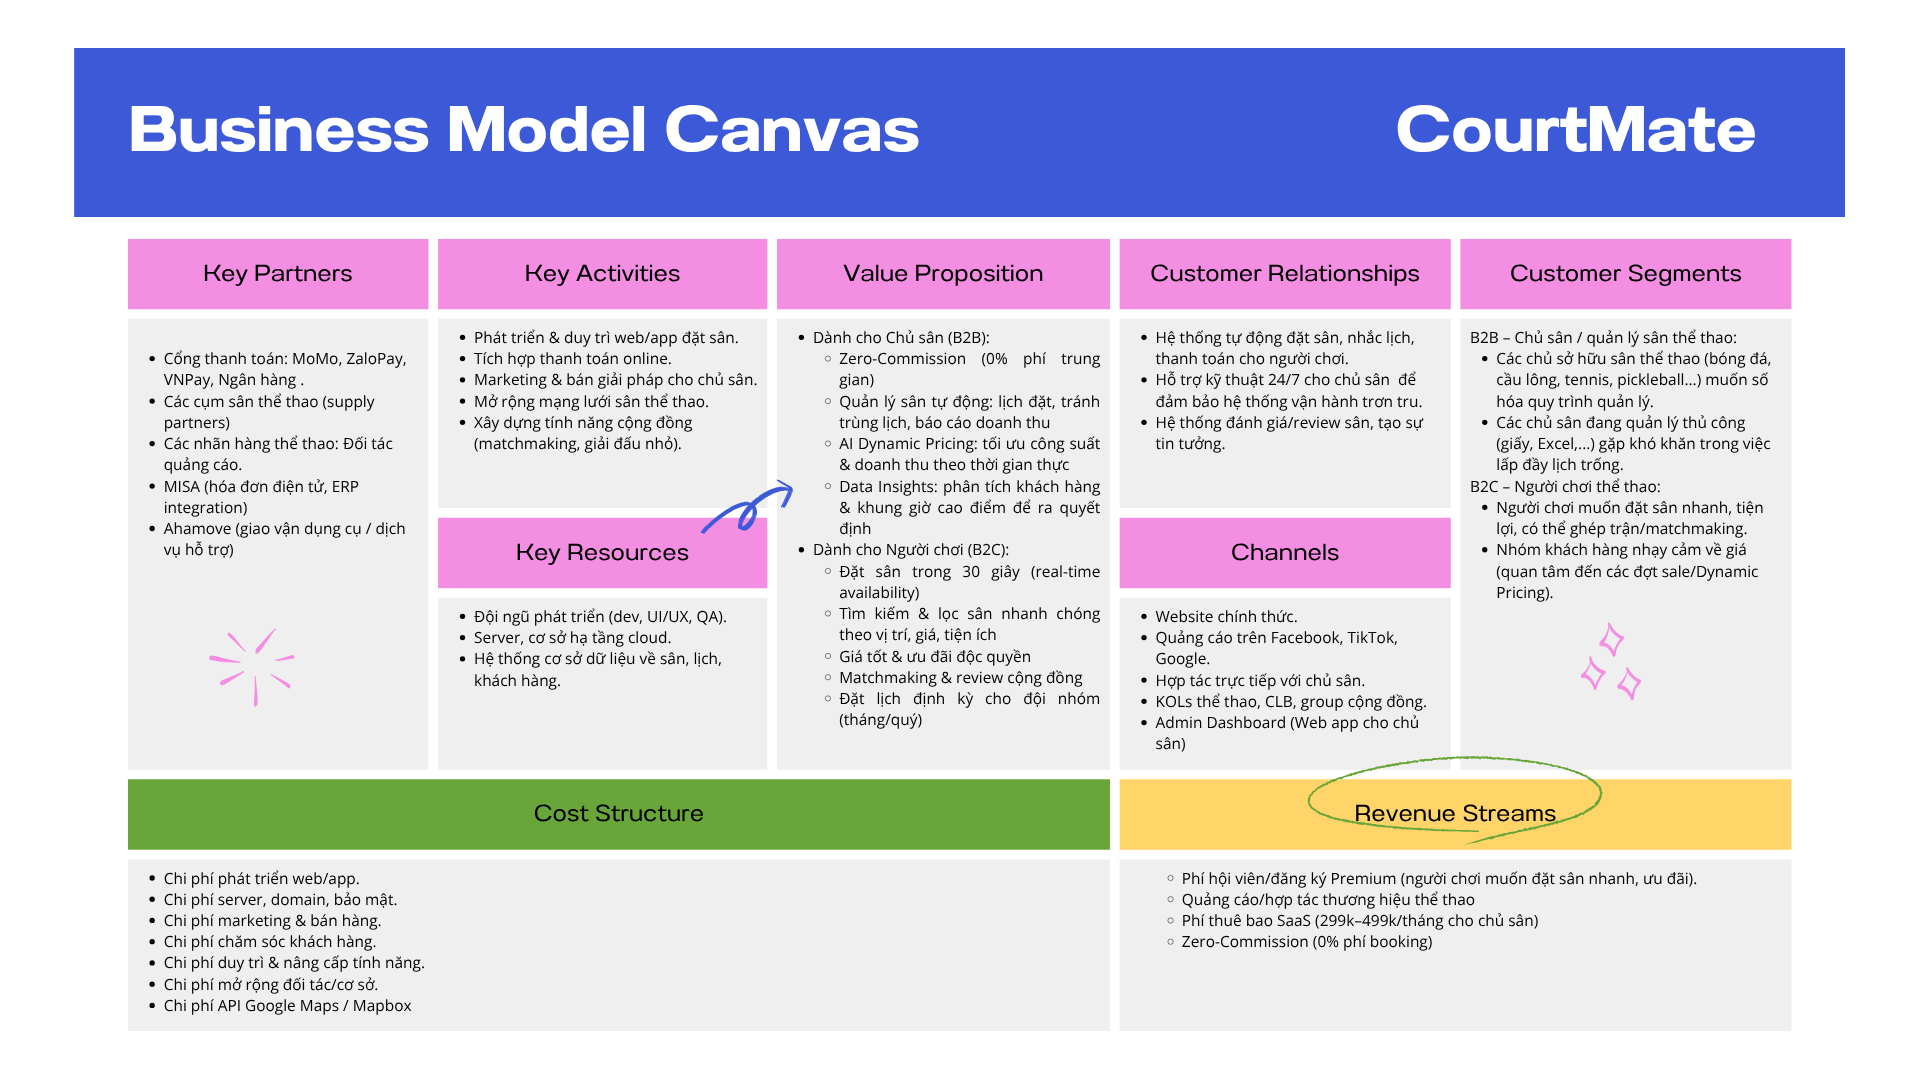
\includegraphics[width=1\textwidth]{Images/BMC.png}
    \caption{Khung mô hình kinh doanh (Business Model Canvas) của hệ thống CourtMate}
    \label{fig:bmc}
\end{figure}


\subsection{Chi tiết các thành phần trong mô hình}

\begin{enumerate}
    \item \textbf{Phân khúc khách hàng (Customer Segments):}
    \begin{itemize}
        \item \textbf{B2B (Chủ sân/Người quản lý):} Các chủ sở hữu cụm sân thể thao cần công cụ quản lý chuyên nghiệp, tự động hóa và báo cáo tài chính chính xác.
        \item \textbf{B2C (Người chơi thể thao):} Cá nhân hoặc nhóm người chơi cần tìm kiếm và đặt sân nhanh chóng, minh bạch về giá cả và tiện ích.
    \end{itemize}

    \item \textbf{Giải pháp giá trị (Value Propositions):}
    \begin{itemize}
        \item \textbf{Cho chủ sân:} Giảm thiểu sai sót thủ công, tối ưu hóa công suất khai thác sân (đặc biệt là giờ thấp điểm), quản lý tài chính tích hợp hóa đơn điện tử.
        \item \textbf{Cho người chơi:} Trải nghiệm đặt sân trong 30 giây; hiển thị trạng thái sân thời gian thực; tích hợp thanh toán linh hoạt; hệ thống Matchmaking tự động ghép trận và tính năng Recurring Booking cho phép đặt lịch cố định dài hạn.
    \end{itemize}

    \item \textbf{Các kênh truyền thông và phân phối (Channels):}
    \begin{itemize}
        \item Ứng dụng Web/Mobile cho người chơi.
        \item Bảng điều khiển (Admin Panel) chuyên dụng cho chủ sân.
        \item Mạng xã hội và các diễn đàn cộng đồng thể thao.
    \end{itemize}

    \item \textbf{Quan hệ khách hàng (Customer Relationships):}
    \begin{itemize}
        \item Hỗ trợ kỹ thuật 24/7 cho các chủ sân SaaS.
        \item Hệ thống đánh giá và phản hồi đa chiều giữa người chơi và chủ sân.
    \end{itemize}

    \item \textbf{Dòng doanh thu (Revenue Streams):}
    \begin{itemize}
        \item \textbf{B2B (SaaS):} Phí thuê bao hàng tháng từ chủ sân với cam kết 0\% hoa hồng, giúp họ tối ưu hóa lợi nhuận biên.
        \item \textbf{B2C (Premium):} Gói hội viên cao cấp dành cho người chơi để nhận ưu đãi, quét mã giảm giá và miễn phí phí ghép trận.
        \item \textbf{B2B2C (Ads):} Doanh thu quảng cáo từ các thực thể thương mại và nhãn hàng thể thao tài trợ.
    \end{itemize}

    \item \textbf{Các hoạt động chính (Key Activities):}
    \begin{itemize}
        \item Phát triển và bảo trì nền tảng kỹ thuật.
        \item Kết nối và mở rộng mạng lưới các đối tác cụm sân.
        \item Tiếp thị và chăm sóc khách hàng.
    \end{itemize}

    \item \textbf{Các nguồn lực chính (Key Resources):}
    \begin{itemize}
        \item Đội ngũ kỹ sư phát triển phần mềm.
        \item Hạ tầng máy chủ Cloud và cơ sở dữ liệu.
        \item Dữ liệu về bản đồ và vị trí các cụm sân.
    \end{itemize}

    \item \textbf{Các đối tác chính (Key Partners):}
    \begin{itemize}
        \item \textbf{Thanh toán:} MoMo, ZaloPay xử lý giao dịch tức thời và bảo mật.
        \item \textbf{Công nghệ \& Vận hành:} MISA meInvoice (hóa đơn điện tử); Ahamove (giao vận dụng cụ/nhu yếu phẩm).
        \item \textbf{Thương mại:} Các nhãn hàng thể thao tài trợ và quảng cáo trên nền tảng.
    \end{itemize}

    \item \textbf{Cơ cấu chi phí (Cost Structure):}
    \begin{itemize}
        \item Chi phí vận hành hạ tầng Cloud (AWS/Azure).
        \item Phí sử dụng API Google Maps.
        \item Chi phí nhân sự và Marketing.
    \end{itemize}
\end{enumerate}

\newpage
% \section{Chiến lược bán hàng và Cạnh tranh}

\subsection{Chiến lược định giá và Tối ưu doanh thu (Pricing \& Monetization Strategy)}
Hệ thống CourtMate áp dụng mô hình doanh thu phức hợp (Hybrid Monetization) nhằm tối ưu hóa dòng tiền từ cả hai phía cung và cầu, đồng thời tạo ra rào cản gia nhập thị trường đối với các đối thủ cạnh tranh. Chiến lược này được phân rã thành ba luồng giá trị cốt lõi:

\begin{enumerate}
    \item \textit{Phân khúc B2B (Chủ sân):} Hệ thống triển khai mô hình SaaS (Software-as-a-Service) dựa trên các gói thuê bao linh hoạt (Tier-based Pricing). Điểm khác biệt lớn nhất là cam kết Zero-Commission (0\% phí hoa hồng trên mỗi giao dịch). Thay vì trích phần trăm doanh thu như các nền tảng trung gian, CourtMate thu phí duy trì hệ thống cố định, giúp chủ sân tối ưu hóa lợi nhuận biên và khuyến khích họ đưa toàn bộ quỹ sân lên hệ thống trực tuyến.
    \item \textit{Phân khúc B2C (Người chơi):} Cung cấp gói Hội viên Premium để tạo doanh thu ổn định (Recurring Revenue). Người dùng Premium hưởng các đặc quyền như đặt lịch không cần cọc (Hold-without-deposit), ưu tiên ghép trận và các voucher từ đối tác thương mại.
    \item \textit{AI Dynamic Pricing:} Thuật toán AI hoạt động như một công cụ Yield Management tự động. Hệ thống sẽ điều chỉnh giá thuê sân theo thời gian thực dựa trên thời tiết và mật độ occupancy — tăng giá vào giờ cao điểm và giảm giá sâu vào giờ thấp điểm để giảm thiểu chi phí cơ hội.
\end{enumerate}

\subsection{Lợi thế cạnh tranh độc quyền (Unique Selling Propositions - USP)}
CourtMate định vị mình là giải pháp dẫn đầu thị trường nhờ vào các lợi thế cạnh tranh mang tính bản địa hóa và công nghệ vượt trội:
\begin{itemize}
    \item \textit{Localized Integration:} Tích hợp sâu với các cổng thanh toán VietQR và đặc biệt là hệ thống hóa đơn điện tử MISA. Đây là rào cản kỹ thuật mà các ứng dụng quốc tế khó vượt qua tại thị trường Việt Nam.
    \item \textit{Data-Driven Insights:} Cung cấp cho chủ sân các công cụ phân tích dữ liệu trực quan như Bản đồ nhiệt (Heatmap) về tỷ lệ lấp đầy và báo cáo tài chính thời gian thực.
    \item \textit{Hybrid Sports Support:} Hỗ trợ cấu hình lưới lịch linh hoạt cho các môn thể thao lai như Pickleball, cho phép chia nhỏ hoặc gộp sân một cách nhanh chóng.
\end{itemize}

\subsection{Phân tích đối thủ cạnh tranh (Competitor Analysis Matrix)}
Dưới đây là bảng so sánh CourtMate với các nhóm đối thủ chính dựa trên các tiêu chí vận hành thực tế:

\begin{table}[H]
    \centering
    \renewcommand{\arraystretch}{1.3}
    \begin{tabularx}{\textwidth}{|>{\raggedright\arraybackslash}p{2.5cm}|c|X|X|X|}
    \hline
    \textbf{Tiêu chí} & \textbf{CourtMate} & \textbf{Nền tảng Quốc tế \cite{ref:playtomic, ref:courtreserve}} & \textbf{Giải pháp Nội địa \cite{ref:alobo}} & \textbf{Quản lý truyền thống} \\ \hline
    Chi phí sử dụng & Phí SaaS thấp & Phí SaaS cao (199\$-549\$/th) \cite{ref:playtomic, ref:courtreserve} & Phí SaaS trung bình (220k-299k) \cite{ref:alobo} & Miễn phí \\ \hline
    Tự động hóa AI & Cao (Dynamic Pricing) & Trung bình & Không hỗ trợ định giá động & Không hỗ trợ \\ \hline
    Bản địa hóa & Tối ưu (VietQR) & Hạn chế \cite{ref:playtomic, ref:courtreserve} & Tốt (Thanh toán VN) & Thủ công \\ \hline
    Trải nghiệm UX & Mượt mà, đa dịch vụ & Chuyên nghiệp & Phổ thông, tập trung POS & Phụ thuộc nhân sự \\ \hline
    \end{tabularx}
    \caption{Ma trận so sánh năng lực cạnh tranh}
    \label{tab:competitor_matrix}
\end{table}

\subsection{Cơ sở dữ liệu và Động lực định giá (Pricing Rationale \& Data-Driven)}
Để đảm bảo tính khả thi tài chính và đáp ứng tiêu chí định giá dựa trên dữ liệu thực tế, mức phí gói SaaS B2B của CourtMate (dao động từ 200.000 VNĐ - 500.000 VNĐ/tháng tùy quy mô cụm sân) được thiết lập dựa trên phân tích khả năng chi trả (Willingness-to-pay) của các doanh nghiệp SME tại Việt Nam:

\begin{itemize}
    \item \textbf{Benchmark thị trường chéo (Cross-industry Benchmark):} Dựa trên dữ liệu khảo sát biểu phí của các giải pháp quản lý bán lẻ và F\&B phổ biến trên thị trường như KiotViet hay PosApp (hiện đang thu phí dao động từ 220.000 - 299.000 VNĐ/tháng cho gói cơ bản), mức giá đề xuất của CourtMate hoàn toàn nằm trong ngưỡng an toàn, cạnh tranh và dễ dàng gỡ bỏ rào cản chi phí cho các chủ sân.
    \item \textbf{Chiến lược Thâm nhập thị trường (Market Penetration):} Động lực cốt lõi của chính sách Zero-Commission (0\% hoa hồng) không phải là hi sinh biên lợi nhuận, mà là vũ khí chiến lược để thu hút nhanh chóng nguồn cung. Khi nền tảng đạt được Điểm tới hạn (Critical Mass) về số lượng sân bãi, CourtMate sẽ sở hữu một lượng lớn dữ liệu người chơi (B2C) tự nhiên. Nguồn dữ liệu hành vi này chính là tài nguyên để khai thác luồng doanh thu mở rộng về sau: Quảng cáo nhắm mục tiêu (Ad-supported) cho các thương hiệu dụng cụ thể thao.
\end{itemize}

% \newpage
% \section{Tiếp thị và Quảng cáo}

\subsection{Tiếp thị B2B (Dành cho chủ sân)}
Chiến lược tiếp thị dành cho nhóm khách hàng doanh nghiệp (B2B) của CourtMate tập trung vào việc chuyển đổi tư duy quản lý truyền thống sang nền tảng số hóa thông qua hai kênh chính:
\begin{enumerate}
    \item \textit{Direct Sales \& Demo:} Đội ngũ phát triển trực tiếp tiếp cận các chủ sân, cung cấp các buổi mô phỏng hiển thị dữ liệu thực tế trên bảng điều khiển. Đối với mô hình phần mềm SaaS B2B, các chủ sân thường có tâm lý ngại thay đổi do lo sợ sự phức tạp của công nghệ. Việc trình diễn trực tiếp khả năng xử lý đơn giản và tính bảo mật cao của hệ thống giúp phá vỡ các rào cản tâm lý này, đồng thời chứng minh được giá trị thực tế của việc tự động hóa \cite{ref:gartner}.
    \item \textit{Referral Program:} Tận dụng mạng lưới quan hệ trong cộng đồng kinh doanh thể thao, hệ thống áp dụng cơ chế giảm phí duy trì cho các chủ sân khi họ giới thiệu thành công các cụm sân khác gia nhập hệ sinh thái CourtMate. 
\end{enumerate}

\subsection{Tiếp thị B2C (Dành cho người chơi)}
Chiến lược tiếp thị dành cho người dùng cuối (B2C) tập trung vào việc tạo ra sự hiện diện tối đa tại các điểm chạm kỹ thuật số:
\begin{itemize}
    \item \textit{SEO Local:} Tối ưu hóa các cụm từ tìm kiếm mang tính vị trí như "đặt sân pickleball gần đây". Việc xuất hiện tại các vị trí đầu trên kết quả tìm kiếm tự nhiên giúp thu hút tệp khách hàng có nhu cầu thực và đang ở gần cụm sân nhất.
    \item \textit{Community Building:} Thể thao là lĩnh vực có tính kết nối cộng đồng cực kỳ cao. Dự án tập trung phát triển các kênh TikTok và Group Facebook chuyên về review sân bãi và tổ chức giải đấu ảo. Tại Việt Nam, mạng xã hội dạng video ngắn (TikTok) và cộng đồng Facebook là những công cụ tiếp cận người dùng Gen Z và Gen Y hiệu quả nhất \cite{ref:wearesocial}.
\end{itemize}

\subsection{Chiến lược quảng cáo trả phí (Paid Ads)}
Chiến lược quảng cáo được triển khai dựa trên cơ chế Quảng cáo theo vị trí địa lý (Geo-targeting Ads) trên Google và Facebook. Do đặc thù người chơi thường chỉ tìm kiếm sân trong bán kính 5-10km xung quanh khu vực làm việc và sinh sống, việc chạy quảng cáo theo vị trí kết hợp tung mã giảm giá giờ thấp điểm sẽ giúp tối ưu hóa tỷ lệ chuyển đổi (Conversion Rate) và tiết kiệm ngân sách tiếp thị \cite{ref:kotler}.

\subsection{Hệ thống KPI và Đo lường hiệu quả (KPIs \& Metrics)}
Để kiểm soát và đánh giá tính hiệu quả của chiến lược tiếp thị đa kênh (Omnichannel) trong 6 tháng đầu triển khai (Giai đoạn Go-to-Market), dự án thiết lập hệ thống KPI đo lường cụ thể cho từng phân khúc:
\begin{itemize}
    \item \textbf{Chỉ số đo lường mảng B2B (Chủ sân):}
    \begin{itemize}
        \item \textit{Tốc độ tăng trưởng đối tác:} Ký kết và triển khai thành công phần mềm cho 50 cụm sân (khoảng 200 sân lẻ) tại khu vực TP.HCM.
        \item \textit{Tỷ lệ rời bỏ (Churn Rate):} Duy trì mức dưới 5\%/tháng sau khi kết thúc gói dùng thử (Freemium 1-3 tháng).
    \end{itemize}
    \item \textbf{Chỉ số đo lường mảng B2C (Người chơi):}
    \begin{itemize}
        \item \textit{Chi phí thu thập khách hàng (CAC - Customer Acquisition Cost):} Tối ưu hóa các chiến dịch Local SEO và Referral để đưa CAC xuống dưới 20.000 VNĐ/người dùng mới.
        \item \textit{Tỷ lệ chuyển đổi (Conversion Rate):} Đạt mức tối thiểu 15\% (Cứ 100 người dùng tải ứng dụng hoặc truy cập website sẽ có ít nhất 15 người thực hiện đặt sân và thanh toán thành công).
    \end{itemize}
    \item \textbf{Chỉ số Quảng cáo (Paid Ads):} Đạt tỷ suất lợi nhuận trên chi phí quảng cáo (ROAS - Return on Ad Spend) $> 2.5$ đối với các chiến dịch Geo-targeting trên nền tảng Facebook và TikTok.
\end{itemize}
% \newpage
% \section{Quản trị tài chính và Nguồn lực}

\subsection{Dự toán tài chính chi tiết}
Hệ thống tài chính của CourtMate được xây dựng để hỗ trợ mô hình kinh doanh B2B SaaS (Phần mềm dịch vụ dành cho doanh nghiệp), tập trung vào việc tối ưu hóa dòng tiền và duy trì lợi thế cạnh tranh "Zero-Commission".
\subsubsection{Vốn đầu tư ban đầu (CAPEX)}
Đây là nguồn vốn tập trung vào việc xây dựng nền tảng từ đầu đến khi sẵn sàng tung ra thị trường (giai đoạn MVP)
\begin{itemize}
    \item Chi phí Nghiên cứu và Phát triển (R\&D): dao động khoảng 150 - 200 triệu VNĐ. Khoản này chi trả cho việc thiết kế kiến trúc hệ thống, xây dựng các quy trình nghiệp vụ đặt sân và đảm bảo tính bảo mật dữ liệu.
    \item Thiết lập hạ tầng máy chủ: triển khai mô hình Multi-Cloud để tận dụng tốc độ của nhà cung cấp trong nước và sự ổn định của hệ thống quốc tế.
\end{itemize}

\subsubsection{Chi phí vận hành hàng tháng (OPEX)}
\noindent \textbf{Lựa chọn nhà cung cấp}: nhóm thực hiện đối sánh năng lực giữa các đơn vị cung cấp máy chủ lớn hiện nay
\begin{table}[htbp]
    \centering
    \begin{tabularx}{\textwidth}{@{}l X X X@{}}
        \toprule
        \textbf{Tiêu chí} & \textbf{AWS (Toàn cầu)} & \textbf{Viettel IDC (Nội địa)} & \textbf{Bizfly Cloud (Nội địa)} \\
        \midrule
        Độ trễ & Cao (30-50ms) & Thấp (<10ms) & Thấp (<10ms) \\
        Chi phí tính toán & Khá cao & Trung bình & Thấp (tối ưu nhất) \\
        Quản lý dữ liệu & Ổn định & Đang phát triển & Đang phát triển \\
        Chi phí băng thông & Cao & Miễn phí/Rẻ & Miễn phí/Rẻ \\
        \bottomrule
    \end{tabularx}
    \caption{So sánh năng lực hạ tầng giữa các nhà cung cấp Cloud}
    \label{tab:cloud_comparison}
    \small
\end{table}
\\ 
\noindent Nhóm chọn kết hợp Bizfly Cloud để vận hành các tính năng hằng ngày nhằm giảm chi phí và tăng tốc độ, đồng thời dùng Amazon (AWS) để lưu trữ dữ liệu quan trọng nhằm đảm bảo tính an toàn tuyệt đối.         
\\ \\ \\
\noindent Dựa trên sự kết hợp giữa các nhà cung cấp, chi phí phần cứng để vận hành hệ thống được cụ thể hóa như sau
\begin{table}[htbp]
    \centering
    \begin{tabularx}{\textwidth}{@{}l l r r@{}}
        \toprule
        \textbf{Hạng mục} & \textbf{Nhà cung cấp} & \textbf{Đơn giá/Tháng} & \textbf{Tổng 12 tháng (VNĐ)} \\
        \midrule
        Tính toán & Bizfly Cloud (Basic) & 300.000 & 3.600.000 \\
        Quản lý dữ liệu & AWS & 450.000 & 5.400.000 \\
        Lưu trữ \& CDN & AWS S3 \& Cloudflare & 150.000 & 1.800.000 \\
        \midrule
        \multicolumn{3}{@{}l}{\textbf{Tổng chi phí dự kiến}} & \textbf{10.800.000} \\
        \bottomrule
    \end{tabularx}
    \caption{Dự toán chi tiết hạ tầng Cloud năm thứ nhất}
    \label{tab:cloud_budget_year1}
    \small
\end{table}
\\ \\ \\
Để duy trì dịch vụ cho 80 cụm sân, dự toán chi phí hàng tháng được phân bổ như sau:
\begin{table}[H]
    \centering
    \begin{tabularx}{\textwidth}{@{}l X r@{}}
        \toprule
        \textbf{Hạng mục} & \textbf{Mô tả chi tiết} & \textbf{Dự toán (VNĐ)} \\
        \midrule
        Hệ thống lưu trữ \& Kết nối & Duy trì máy chủ, cơ sở dữ liệu khách hàng, bản đồ số và hệ thống gửi thông báo/SMS cho chủ sân & 2.500.000 \\
        \addlinespace
        Tiếp thị \& Phát triển thị trường & Chi phí tìm kiếm khách hàng (chủ sân), quảng cáo trên mạng xã hội và các chương trình khuyến khích giới thiệu người dùng mới & 10.000.000 \\
        \addlinespace
        Quản lý \& Hỗ trợ kỹ thuật & Chi phí nhân sự trực tuyến để giải quyết các vấn đề kỹ thuật phát sinh và hỗ trợ chủ sân vận hành phần mềm & 15.000.000 \\
        \midrule
        \textbf{Tổng chi phí} & & \textbf{27.500.000} \\
        \bottomrule
    \end{tabularx}
    \caption{Dự toán chi phí vận hành hàng tháng (OPEX)}
    \label{tab:opex_estimate}
    \small
\end{table}

\subsubsection{Mô hình doanh thu và Điểm hòa vốn}
Nền tảng vận hành theo mô hình cung cấp phần mềm dưới dạng dịch vụ thuê bao định kỳ (SaaS). Chủ sân không cần trả hoa hồng trên mỗi lượt khách đặt, thay vào đó sẽ trả phí duy trì cố định để dễ dàng quản lý lợi nhuận. \\ 

\noindent Các gói dịch vụ dành cho chủ sân: được thiết kế phù hợp với quy mô kinh doanh của từng cụm sân
\begin{itemize}
    \item \textbf{Gói Tiêu chuẩn (Standard)}: dành cho các cụm dưới 5 sân, mức phí 299.000 VNĐ/tháng.
    \item \textbf{Gói Doanh nghiệp (Enterprise)}: dành cho các cụm trên 5 sân, mức phí 499.000 VNĐ/tháng.
\end{itemize} 
\vspace{0.5cm}
\noindent Ước tính doanh thu hàng tháng khi hệ thống đạt quy mô 80 cụm sân (giả định 60\% gói Enterprise và 40\% gói Standard)
\begin{itemize}
    \item \textbf{Doanh thu từ phí dịch vụ (SaaS)}: uớc tính đạt 33.520.000 VNĐ/tháng (48 $\times$ 499.000 + 32 $\times$ 299.000)
    \item \textbf{Doanh thu từ quảng cáo}: uớc tính 5.000.000 VNĐ/tháng từ việc hiển thị thương hiệu của các nhãn hàng thể thao tại các vị trí ưu tiên trên hệ thống.
    \item \textbf{Lợi nhuận ròng}: sau khi trừ mọi chi phí, hệ thống mang về lợi nhuận khoảng 11.020.000 VNĐ/tháng.
    \item \textbf{Thời gian hoàn vốn}: với tổng vốn đầu tư ban đầu ước tính 150 - 200 triệu VNĐ, dự án dự kiến đạt điểm hòa vốn sau 14 - 18 tháng hoạt động ổn định.
\end{itemize}


\subsection{Cơ cấu tổ chức và Mô tả công việc}
\subsubsection{Sơ đồ tổ chức theo giai đoạn phát triển}
Cơ cấu nhân lực của CourtMate được chia làm 2 giai đoạn để tối ưu hóa chi phí nhân sự:
\begin{enumerate}
    \item \textbf{Giai đoạn Xây dựng (Startup/MVP)}: tập trung 100\% vào đội ngũ kỹ sư để hoàn thiện sản phẩm.
    \item \textbf{Giai đoạn Vận hành (Scale-up)}: giữ nguyên đội ngũ kỹ thuật và bổ sung bộ phận kinh doanh (Sales) để trực tiếp tiếp cận các chủ sân.
\end{enumerate}

\subsubsection{Mô tả công việc các vị trí cốt lõi}
Để đảm bảo tính chuyên môn hóa, các thành viên được phân bổ nhiệm vụ theo hướng hỗ trợ mô hình kinh doanh:
\begin{itemize}
    \item \textbf{Hệ thống lõi (Backend Lead - Trần Thanh Phúc)}: thiết kế và vận hành logic của hệ thống, đảm bảo quy trình đặt sân, hủy sân và báo cáo tài chính diễn ra chính xác.
    \item \textbf{Trải nghiệm người dùng (Frontend Lead - Trần Minh Quân)}: phụ trách phát triển về giao diện quản lý lịch sân (kéo-thả) giúp chủ sân thao tác dễ dàng và theo dõi các biểu đồ kinh doanh trực quan.
    \item \textbf{Giao diện khách hàng (Frontend Developer - Nguyễn Đăng Khoa)}: xây dựng các tính năng tìm kiếm sân trên bản đồ, quy trình đăng ký thông tin sân và hệ thống quét mã QR để khách hàng check-in tại sân
    \item \textbf{Bảo mật và Tích hợp (Security \& Integration Engineer - Phạm Văn Quốc Việt)}: đảm bảo an toàn cho tài khoản người dùng, xử lý các giao dịch thanh toán trực tuyến và tích hợp hệ thống hóa đơn điện tử.
    \item \textbf{Kiểm soát Chất lượng \& Vận hành máy chủ (QA/QC \& DevOps - Lê Võ Đăng Khoa)}: kiểm tra lỗi hệ thống trước khi ra mắt, đảm bảo máy chủ luôn hoạt động 24/7 và có khả năng chịu tải cao.
    \item \textbf{Phát triển tính năng bổ trợ (Backend Developer - Nguyễn Trần Bảo Khoa)}: xử lý các nghiệp vụ liên quan đến việc giữ chỗ (lock slot) để tránh tình trạng hai khách hàng đặt trùng một giờ sân, và tối ưu hóa công cụ tìm kiếm sân gần nhất.
\end{itemize}







% \newpage
% \input{Contents/Part3D_Bonus.tex}
% \newpage
\section{Phân tích và Đặc tả Yêu cầu Hệ thống}

\subsection{Xác định các Tác nhân (Actors)}
Dựa trên mô hình kinh doanh nền tảng đa lăng kính (Multi-sided Platform) kết hợp SaaS, hệ thống CourtMate phục vụ ba nhóm tác nhân chính:
\begin{itemize}
    \item \textbf{Người chơi (B2C Customer):} Những cá nhân có nhu cầu tìm kiếm sân thể thao (Pickleball, Cầu lông, Tennis), mong muốn đặt lịch nhanh chóng, tiện lợi và thanh toán trực tuyến.
    \item \textbf{Chủ sân (B2B Partner):} Các đối tác sở hữu cụm sân, cần một hệ thống quản lý lịch trình, cơ sở vật chất, chống thất thoát doanh thu và tối ưu hóa công suất khai thác sân thông qua cấu hình giá động.
    \item \textbf{Quản trị viên hệ thống (System Admin):} Đội ngũ vận hành nền tảng CourtMate, chịu trách nhiệm quản lý tài khoản đối tác, theo dõi dòng tiền và giám sát hoạt động kỹ thuật của hệ thống.
\end{itemize}

\subsection{Biểu đồ Use Case tổng quát}
Biểu đồ Use Case tổng quát thể hiện bức tranh toàn cảnh về cách thức các tác nhân tương tác với hệ thống CourtMate, đảm bảo sự phân tách rõ ràng giữa luồng nghiệp vụ B2C (đặt sân) và B2B (quản lý, vận hành).

\begin{figure}[H]
    \centering
    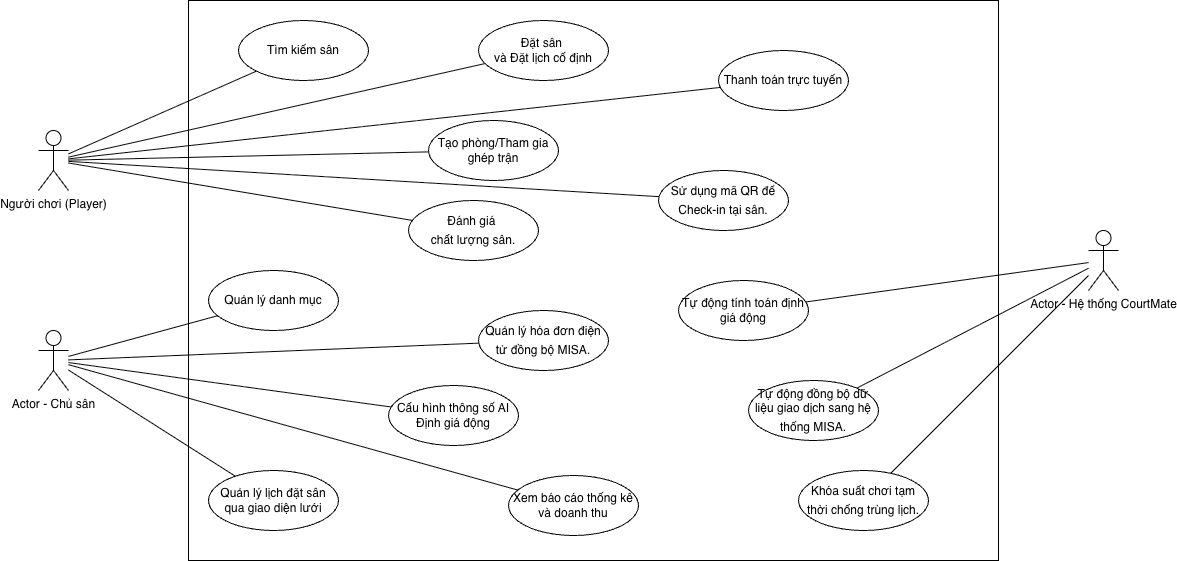
\includegraphics[width=0.95\textwidth]{Images/TMĐT_252-use_case.drawio.png}
    \caption{Biểu đồ Use Case tổng quát của hệ thống CourtMate}
    \label{fig:general_usecase}
\end{figure}

\subsection{Danh sách các Use Case chính}
Hệ thống cung cấp các nhóm chức năng cốt lõi được phân chia theo từng nhóm tác nhân cụ thể. Chi tiết các Use Case được trình bày trong bảng dưới đây:

\begin{table}[H]
    \centering
    \renewcommand{\arraystretch}{1.4}
    \begin{tabular}{|p{4.5cm}|p{3cm}|p{7.5cm}|}
        \hline
        \textbf{Tên Use Case} & \textbf{Tác nhân chính} & \textbf{Mô tả tóm tắt} \\
        \hline
        \multicolumn{3}{|c|}{\textbf{Nhóm: Dành cho Người chơi}} \\
        \hline
        Tìm kiếm sân & Người chơi & Tìm sân theo vị trí, bản đồ không gian và tiện ích. \\
        \hline
        Đặt sân và Đặt lịch cố định & Người chơi & Chọn khung giờ trống để đặt lẻ hoặc đặt cố định định kỳ. \\
        \hline
        Thanh toán trực tuyến & Người chơi & Thực hiện thanh toán khép kín qua MoMo, ZaloPay, VietQR. \\
        \hline
        Tạo phòng/Tham gia ghép trận & Người chơi & Hệ thống Matchmaking giúp người chơi tìm đồng đội cùng trình độ. \\
        \hline
        Check-in tại sân bằng mã QR & Người chơi & Quét mã tại quầy để xác nhận sự hiện diện (Check-in). \\
        \hline
        Đánh giá chất lượng sân & Người chơi & Viết review và chấm điểm sân sau khi hoàn thành buổi chơi. \\
        \hline
        \multicolumn{3}{|c|}{\textbf{Nhóm: Dành cho Chủ sân}} \\
        \hline
        Quản lý danh mục & Chủ sân & Thêm, sửa, xóa thông tin cụm sân (Venue) và các sân lẻ (Court). \\
        \hline
        Quản lý lịch đặt sân & Chủ sân & Kéo-thả trực quan để tạo/dời lịch, nắm bắt trạng thái sân realtime. \\
        \hline
        Cấu hình AI Định giá động & Chủ sân & Thiết lập biên độ giảm/tăng giá, trọng số thời tiết cho AI. \\
        \hline
        Quản lý hóa đơn điện tử & Chủ sân & Quản lý và đối soát các hóa đơn điện tử đã được tự động sinh ra. \\
        \hline
        Xem báo cáo thống kê & Chủ sân & Xem biểu đồ nhiệt (Heatmap), báo cáo tài chính và công suất. \\
        \hline
        \multicolumn{3}{|c|}{\textbf{Nhóm: Hệ thống tự động}} \\
        \hline
        Tính toán định giá động & Hệ thống & AI tự động phân tích dữ liệu và cập nhật hệ số giá (Multiplier). \\
        \hline
        Đồng bộ giao dịch sang MISA & Hệ thống & Gọi API sang MISA xuất hóa đơn ngay sau khi thanh toán. \\
        \hline
        Khóa suất chơi tạm thời & Hệ thống & Cơ chế Optimistic Lock giữ chỗ tạm thời khi khách thanh toán. \\
        \hline
    \end{tabular}
    \caption{Danh sách các Use Case chính của hệ thống CourtMate}
    \label{tab:usecase_list}
\end{table}

\subsection{Đặc tả Use Case trọng tâm: Đặt sân và Thanh toán (B2C)}
\textbf{Tác nhân:} Người chơi \\
\textbf{Mục đích:} Cho phép người chơi tìm kiếm sân trống phù hợp, đặt chỗ và thanh toán trực tuyến trong một luồng duy nhất (Single-page flow).\\
\textbf{Luồng sự kiện chính:}
\begin{enumerate}
    \item Người chơi sử dụng thanh tìm kiếm và bộ lọc để tìm sân trống theo môn thể thao, vị trí, ngày và giờ.
    \item Hệ thống hiển thị danh sách các sân thỏa mãn điều kiện và bản đồ tương tác.
    \item Người chơi chọn một sân và khung giờ cụ thể.
    \item Hệ thống tự động khóa slot (Locking Slot) trong 10 phút để tránh trùng lịch (Race Condition).
    \item Người chơi chọn các dịch vụ đi kèm (nếu có) và tiến hành thanh toán bằng mã QR/Ví điện tử.
    \item Hệ thống nhận Webhook thanh toán thành công, cập nhật trạng thái đơn đặt sân thành "Đã xác nhận".
    \item Hệ thống gửi thông báo xác nhận đến Người chơi và cập nhật ngay lập tức lên Lưới lịch của Chủ sân.
\end{enumerate}

\begin{figure}[H]
    \centering
    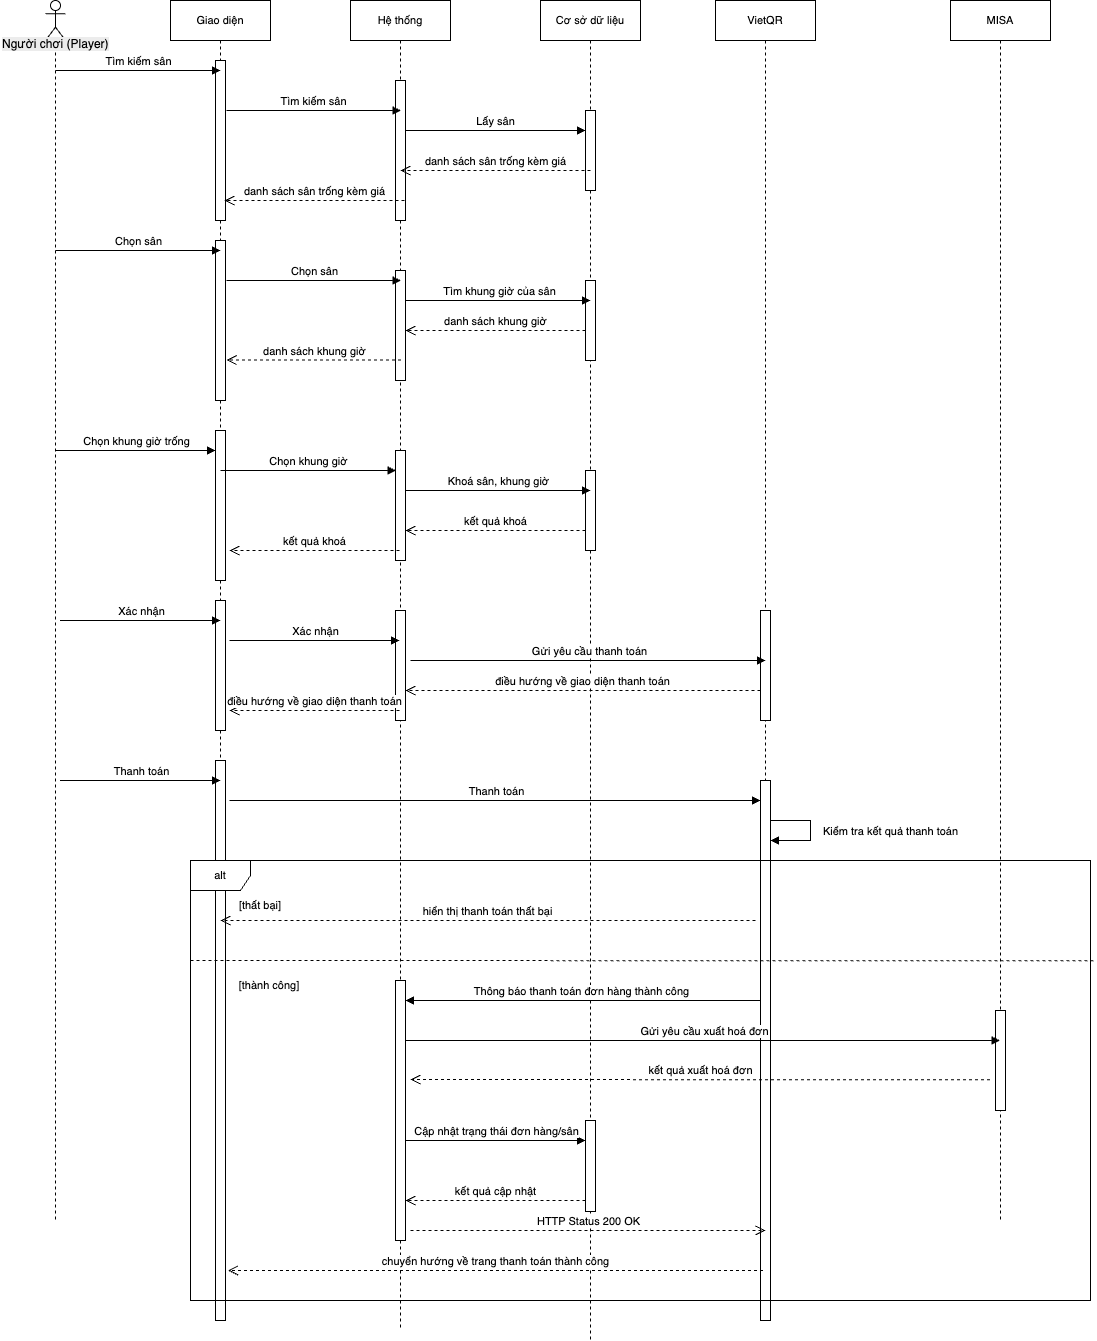
\includegraphics[width=0.95\textwidth]{Images/sq_dat_san_va_thanh_toan.png}
    \caption{Biểu đồ tuần tự (Sequence Diagram) luồng Đặt sân và Thanh toán}
    \label{fig:sequence_booking}
\end{figure}

\subsection{Đặc tả Use Case: Quản lý lưới lịch (Slot Grid) và Định giá}
\textbf{Tác nhân:} Chủ sân \\
\textbf{Mục đích:} Cung cấp công cụ quản trị trực quan để theo dõi, điều chỉnh lịch đặt sân và xử lý các tình huống phát sinh tại sân.\\
\textbf{Luồng sự kiện chính:}
\begin{enumerate}
    \item Chủ sân đăng nhập vào Smart Admin Panel (B2B).
    \item Hệ thống truy xuất dữ liệu và hiển thị Lưới lịch tương tác (Interactive Grid View) theo thời gian thực.
    \item Chủ sân quan sát các slot: màu sắc phân biệt slot đã đặt (online/offline), slot trống, hoặc slot đang bảo trì.
    \item Trong trường hợp khách có nhu cầu đổi giờ hoặc sân gặp sự cố, Chủ sân thực hiện thao tác kéo - thả (Drag-and-drop) slot đặt sân sang một ô trống khác.
    \item Hệ thống kiểm tra tính hợp lệ của slot mới, cập nhật cơ sở dữ liệu và hiển thị thông báo thành công.
\end{enumerate}

\begin{figure}[H]
    \centering
    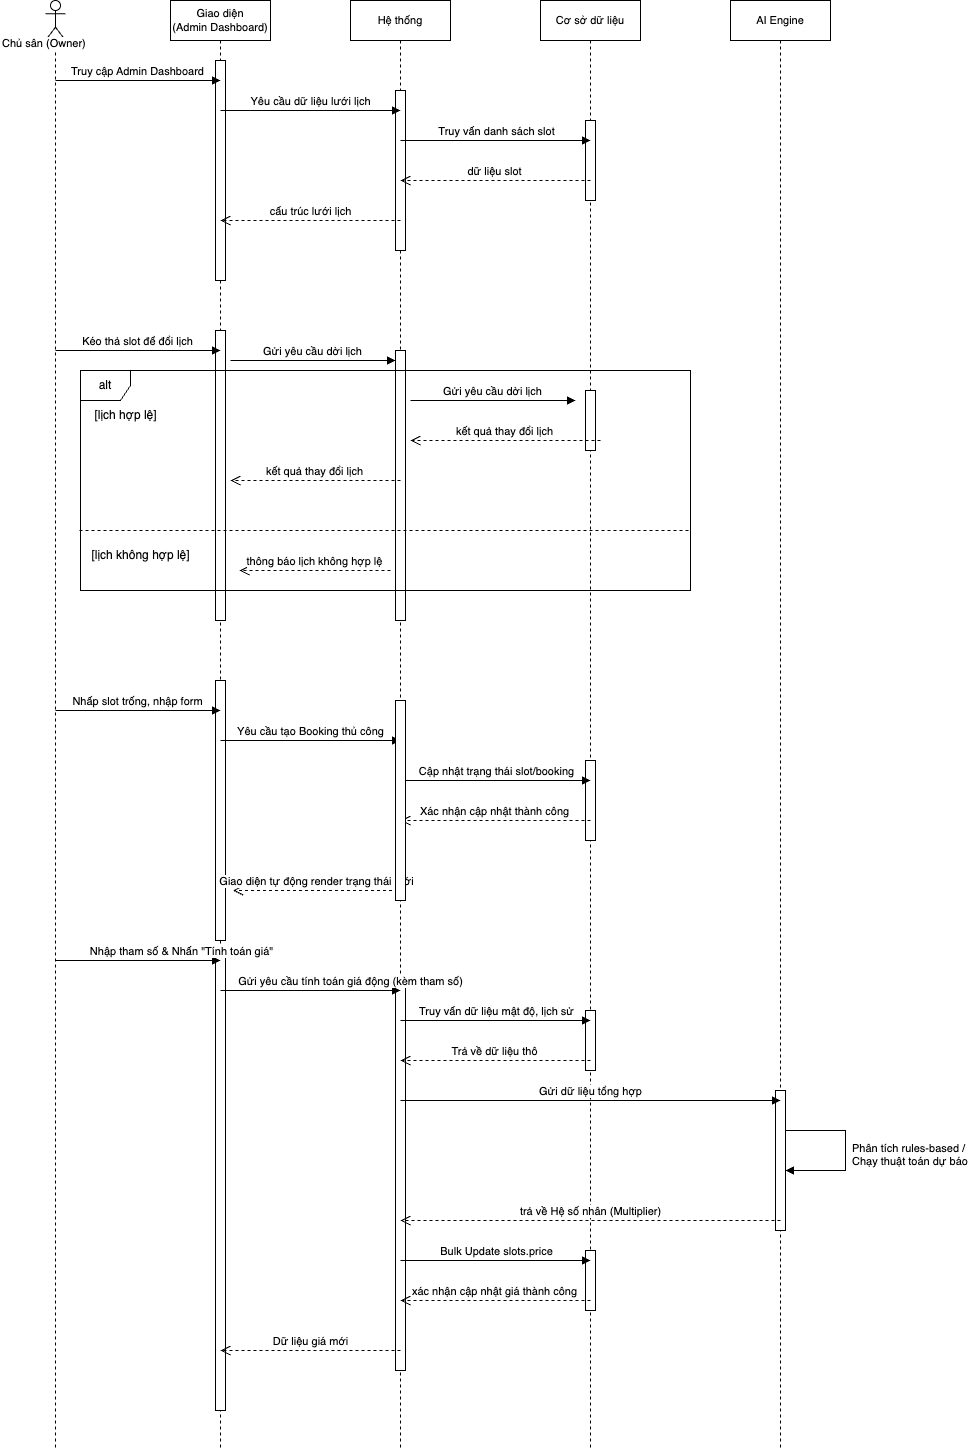
\includegraphics[width=0.95\textwidth]{Images/sq_quan_ly_lich_va_dinh_gia.png}
    \caption{Biểu đồ tuần tự luồng Quản lý lịch và định giá của Chủ sân}
    \label{fig:sequence_slot_management}
\end{figure}

\subsection{Đặc tả Use Case: Sử dụng mã QR để Check-in tại sân (B2C)}
\textbf{Tác nhân:} Người chơi \\
\textbf{Mục đích:} Hỗ trợ người chơi tự động xác nhận sự hiện diện tại quầy một cách nhanh chóng, không cần đối chiếu thủ công. \\
\textbf{Luồng sự kiện chính:}
\begin{enumerate}
    \item Người chơi mở ứng dụng và truy cập vào Đơn đặt sân.
    \item Hệ thống sinh ra và trả về một mã QR Token duy nhất cho đơn hàng.
    \item Người chơi tiến hành quét mã QR này tại thiết bị/quầy của sân.
    \item Mã QR Token được gửi về hệ thống để xác thực. Hệ thống kiểm tra tính hợp lệ của Booking.
    \begin{itemize}
        \item \textbf{Hợp lệ:} Hệ thống cập nhật trạng thái đơn hàng thành "Đã check-in" vào cơ sở dữ liệu và hiển thị thông báo thành công.
        \item \textbf{Không hợp lệ:} Hệ thống hiển thị lỗi "Mã QR không hợp lệ" trên giao diện.
    \end{itemize}
\end{enumerate}

\begin{figure}[H]
    \centering
    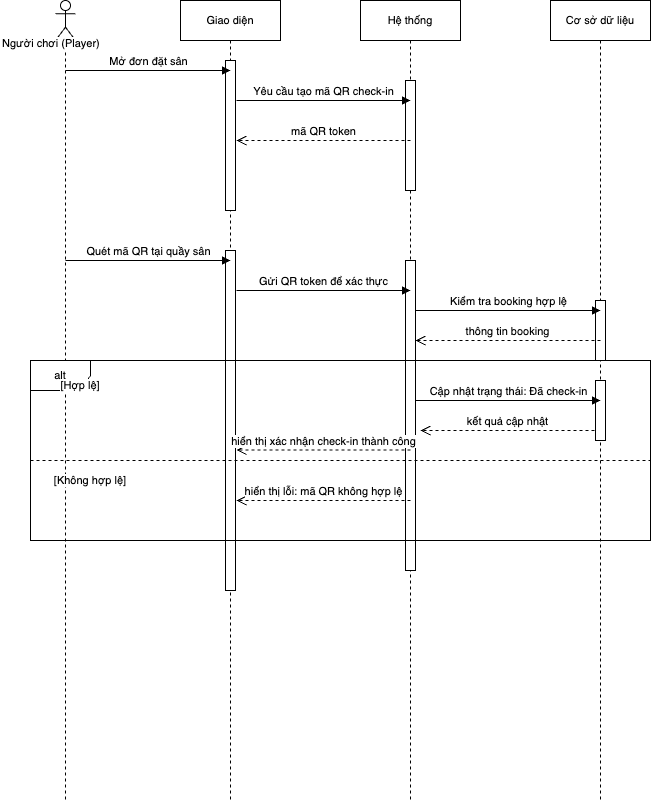
\includegraphics[width=0.95\textwidth]{Images/sq_checkin_qr.png}
    \caption{Biểu đồ tuần tự luồng Sử dụng mã QR để Check-in}
    \label{fig:sequence_checkin}
\end{figure}

\subsection{Đặc tả Use Case: Đánh giá chất lượng sân (B2C)}
\textbf{Tác nhân:} Người chơi \\
\textbf{Mục đích:} Thu thập phản hồi từ khách hàng sau khi trải nghiệm dịch vụ để xây dựng hệ thống xếp hạng uy tín cho các cụm sân. \\
\textbf{Luồng sự kiện chính:}
\begin{enumerate}
    \item Người chơi truy cập vào mục Lịch sử đặt sân.
    \item Hệ thống truy vấn cơ sở dữ liệu và trả về danh sách các Booking có trạng thái "Đã hoàn thành".
    \item Người chơi chọn một Booking cụ thể, nhập điểm số (Rating) và nội dung đánh giá (Review), sau đó nhấn Gửi.
    \item Hệ thống thực hiện Validate (kiểm tra tính hợp lệ) và lưu dữ liệu đánh giá mới.
    \item Hệ thống tự động tính toán lại và cập nhật Điểm trung bình của cụm sân tương ứng.
    \item Trả về thông báo "Đánh giá thành công" trên giao diện người chơi.
\end{enumerate}

\begin{figure}[H]
    \centering
    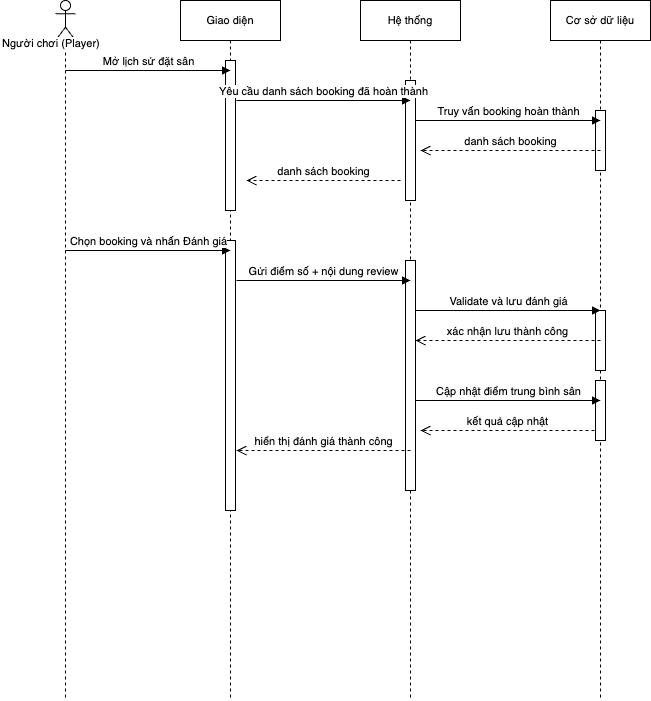
\includegraphics[width=0.95\textwidth]{Images/sq_danh_gia_san.png}
    \caption{Biểu đồ tuần tự luồng Đánh giá chất lượng sân}
    \label{fig:sequence_review}
\end{figure}

\subsection{Đặc tả Use Case: Tạo phòng và Tham gia ghép trận - Matchmaking (B2C)}
\textbf{Tác nhân:} Người chơi \\
\textbf{Mục đích:} Kết nối các cá nhân có cùng trình độ và nhu cầu thời gian để lập nhóm chơi chung, giúp san sẻ chi phí thuê sân. \\
\textbf{Luồng sự kiện chính:}
\begin{enumerate}
    \item Người chơi mở tính năng Ghép trận trên ứng dụng. Hệ thống truy vấn và hiển thị danh sách các phòng đang mở kèm theo thông tin trình độ.
    \item \textbf{Tạo phòng mới:} Người chơi chọn sân, khung giờ, thiết lập yêu cầu trình độ và gửi yêu cầu tạo phòng. Hệ thống lưu thông tin phòng mới, sinh mã phòng và trả về cho người dùng.
    \item \textbf{Tham gia phòng có sẵn:} Người chơi chọn một phòng trong danh sách và nhấn Tham gia. Hệ thống kiểm tra các slot còn trống trong phòng, tiến hành cập nhật trạng thái và trả về thông báo tham gia thành công.
\end{enumerate}

\begin{figure}[H]
    \centering
    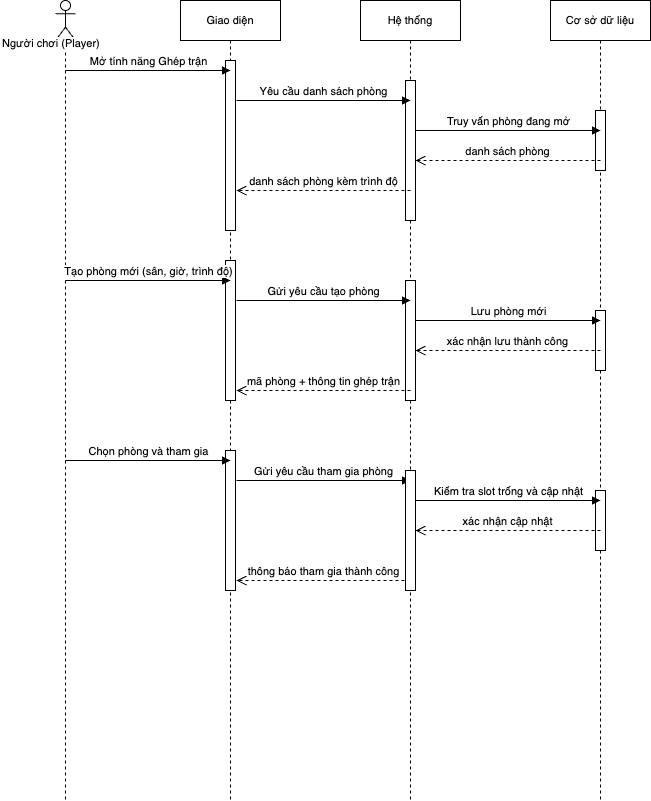
\includegraphics[width=0.95\textwidth]{Images/sq_ghep_tran.png}
    \caption{Biểu đồ tuần tự luồng Tạo phòng và Tham gia ghép trận}
    \label{fig:sequence_matchmaking}
\end{figure}

\subsection{Đặc tả Use Case: Quản lý danh mục sân (B2B)}
\textbf{Tác nhân:} Chủ sân \\
\textbf{Mục đích:} Cho phép chủ sân số hóa cơ sở vật chất, quản lý thông tin các cụm sân (Venue) và sân lẻ (Court) thuộc quyền sở hữu. \\
\textbf{Luồng sự kiện chính:}
\begin{enumerate}
    \item Chủ sân truy cập trang Quản lý danh mục trên Admin Dashboard. Hệ thống trả về danh sách Venue/Court hiện có.
    \item \textbf{Thêm sân:} Chủ sân nhập thông tin (tên, địa chỉ, tiện ích) và gửi yêu cầu. Hệ thống Validate và lưu sân mới vào DB.
    \item \textbf{Sửa thông tin:} Chủ sân chọn sân, cập nhật thông tin và nhấn Gửi. Hệ thống lưu thông tin mới.
    \item \textbf{Xóa sân:} Chủ sân chọn sân và xác nhận xóa. Hệ thống thực hiện lệnh Soft-delete (xóa mềm) trong DB để bảo toàn dữ liệu lịch sử đối soát và trả về kết quả thành công.
\end{enumerate}

\begin{figure}[H]
    \centering
    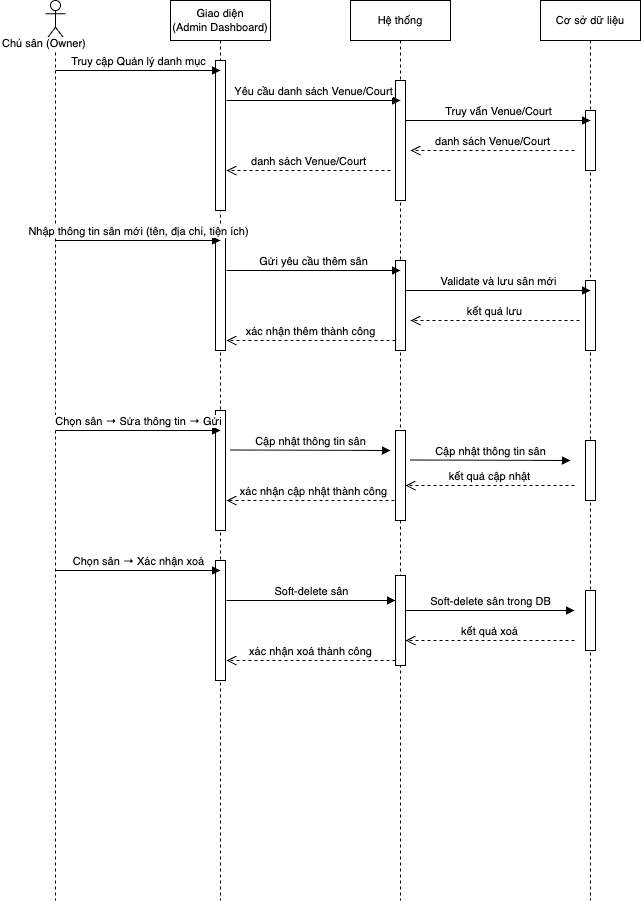
\includegraphics[width=0.95\textwidth]{Images/sq_quan_ly_danh_muc.png}
    \caption{Biểu đồ tuần tự luồng Quản lý danh mục sân}
    \label{fig:sequence_category}
\end{figure}

\subsection{Đặc tả Use Case: Đồng bộ Hóa đơn điện tử MISA (B2B)}
\textbf{Tác nhân:} Chủ sân \\
\textbf{Mục đích:} Tự động hóa quy trình xuất và đối soát hóa đơn điện tử cho các giao dịch đặt sân, đảm bảo tuân thủ pháp lý. \\
\textbf{Luồng sự kiện chính:}
\begin{enumerate}
    \item Chủ sân truy cập trang Hóa đơn. Hệ thống truy vấn và hiển thị danh sách các hóa đơn đã xuất hoặc chờ xử lý.
    \item Chủ sân chọn hóa đơn cần xử lý và nhấn "Đồng bộ MISA".
    \item Hệ thống CourtMate gọi API sang nền tảng MISA meInvoice để yêu cầu xuất hóa đơn.
    \item Sau khi nhận được kết quả từ MISA, hệ thống cập nhật trạng thái hóa đơn tương ứng trong cơ sở dữ liệu và hiển thị thông báo đồng bộ thành công cho Chủ sân.
\end{enumerate}

\begin{figure}[H]
    \centering
    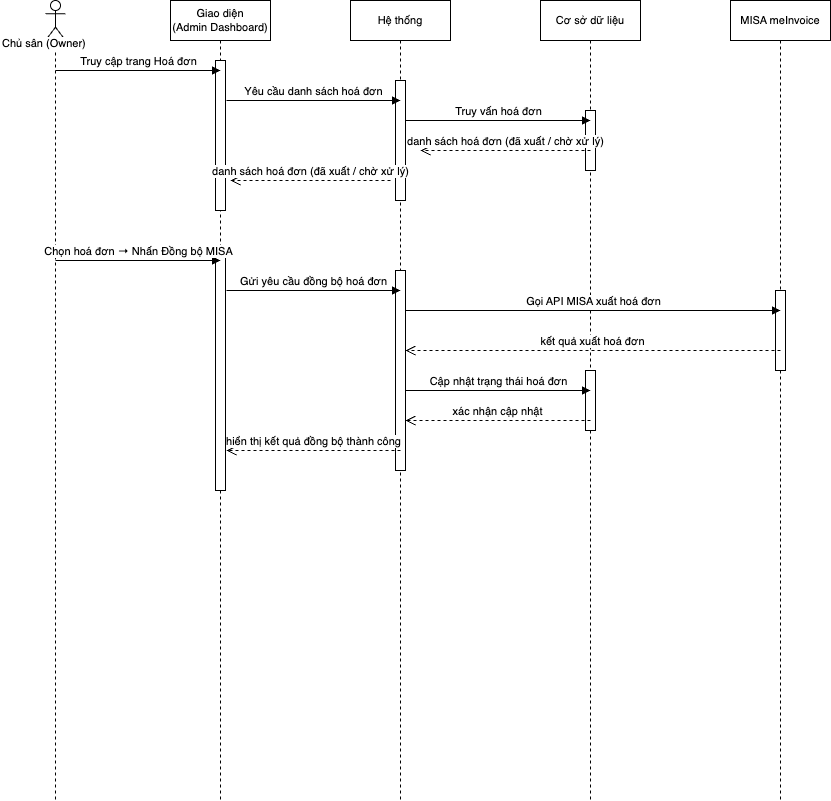
\includegraphics[width=0.95\textwidth]{Images/sq_quan_ly_hoa_don.png}
    \caption{Biểu đồ tuần tự luồng Đồng bộ Hóa đơn điện tử MISA}
    \label{fig:sequence_invoice}
\end{figure}

\subsection{Đặc tả Use Case: Cấu hình AI Định giá động và Xem báo cáo thống kê (B2B)}
\textbf{Tác nhân:} Chủ sân, AI Engine \\
\textbf{Mục đích:} Cung cấp bức tranh toàn cảnh về hiệu quả kinh doanh và cho phép chủ sân áp dụng AI để điều chỉnh giá tự động nhằm tối ưu lợi nhuận. \\
\textbf{Luồng sự kiện chính:}
\begin{enumerate}
    \item \textbf{Xem Báo cáo:} Chủ sân truy cập trang Thống kê. Hệ thống truy vấn và hiển thị Biểu đồ tài chính tổng quan. Khi chọn Biểu đồ nhiệt (Heatmap), hệ thống truy vấn mật độ slot để hiển thị công suất lấp đầy. Chủ sân có thể chọn khoảng thời gian để hệ thống tổng hợp và xuất file báo cáo (PDF/Excel).
    \item \textbf{Cấu hình AI Định giá:} Chủ sân nhập các tham số đầu vào và nhấn "Tính toán giá". Hệ thống tổng hợp dữ liệu (mật độ, lịch sử) và gửi sang AI Engine.
    \item AI Engine thực hiện phân tích rules-based hoặc chạy thuật toán dự báo để tính toán và trả về Hệ số nhân (Multiplier).
    \item Hệ thống thực hiện lệnh Bulk Update để cập nhật hàng loạt trường giá tiền (slots.price) trong cơ sở dữ liệu và tự động render dữ liệu giá mới lên giao diện cho Chủ sân.
\end{enumerate}

\begin{figure}[H]
    \centering
    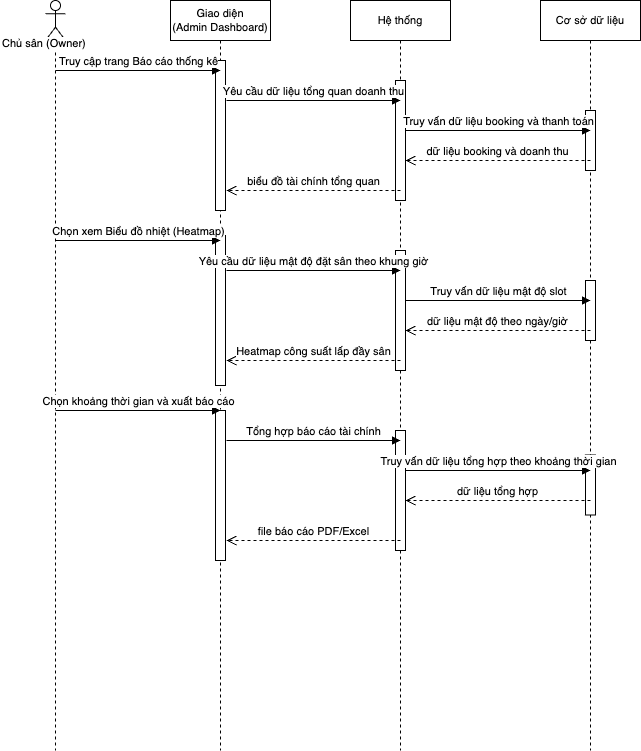
\includegraphics[width=0.95\textwidth]{Images/sq_bao_cao_thong_ke.png}
    \caption{Biểu đồ tuần tự luồng Cấu hình AI Định giá động và Xem báo cáo thống kê}
    \label{fig:sequence_report}
\end{figure}





\section{Kiến trúc hệ thống và Thiết kế kỹ thuật}

\subsection{Kiến trúc tổng thể (High-Level Architecture)}
Hệ thống CourtMate được xây dựng theo kiến trúc Pragmatic Microservices nhằm giải quyết bài toán xử lý lượng truy cập lớn (độ trễ dưới 10ms) nhưng vẫn cân bằng được chi phí vận hành ở giai đoạn sản phẩm tối thiểu (MVP).

\begin{figure}[H]
    \centering
    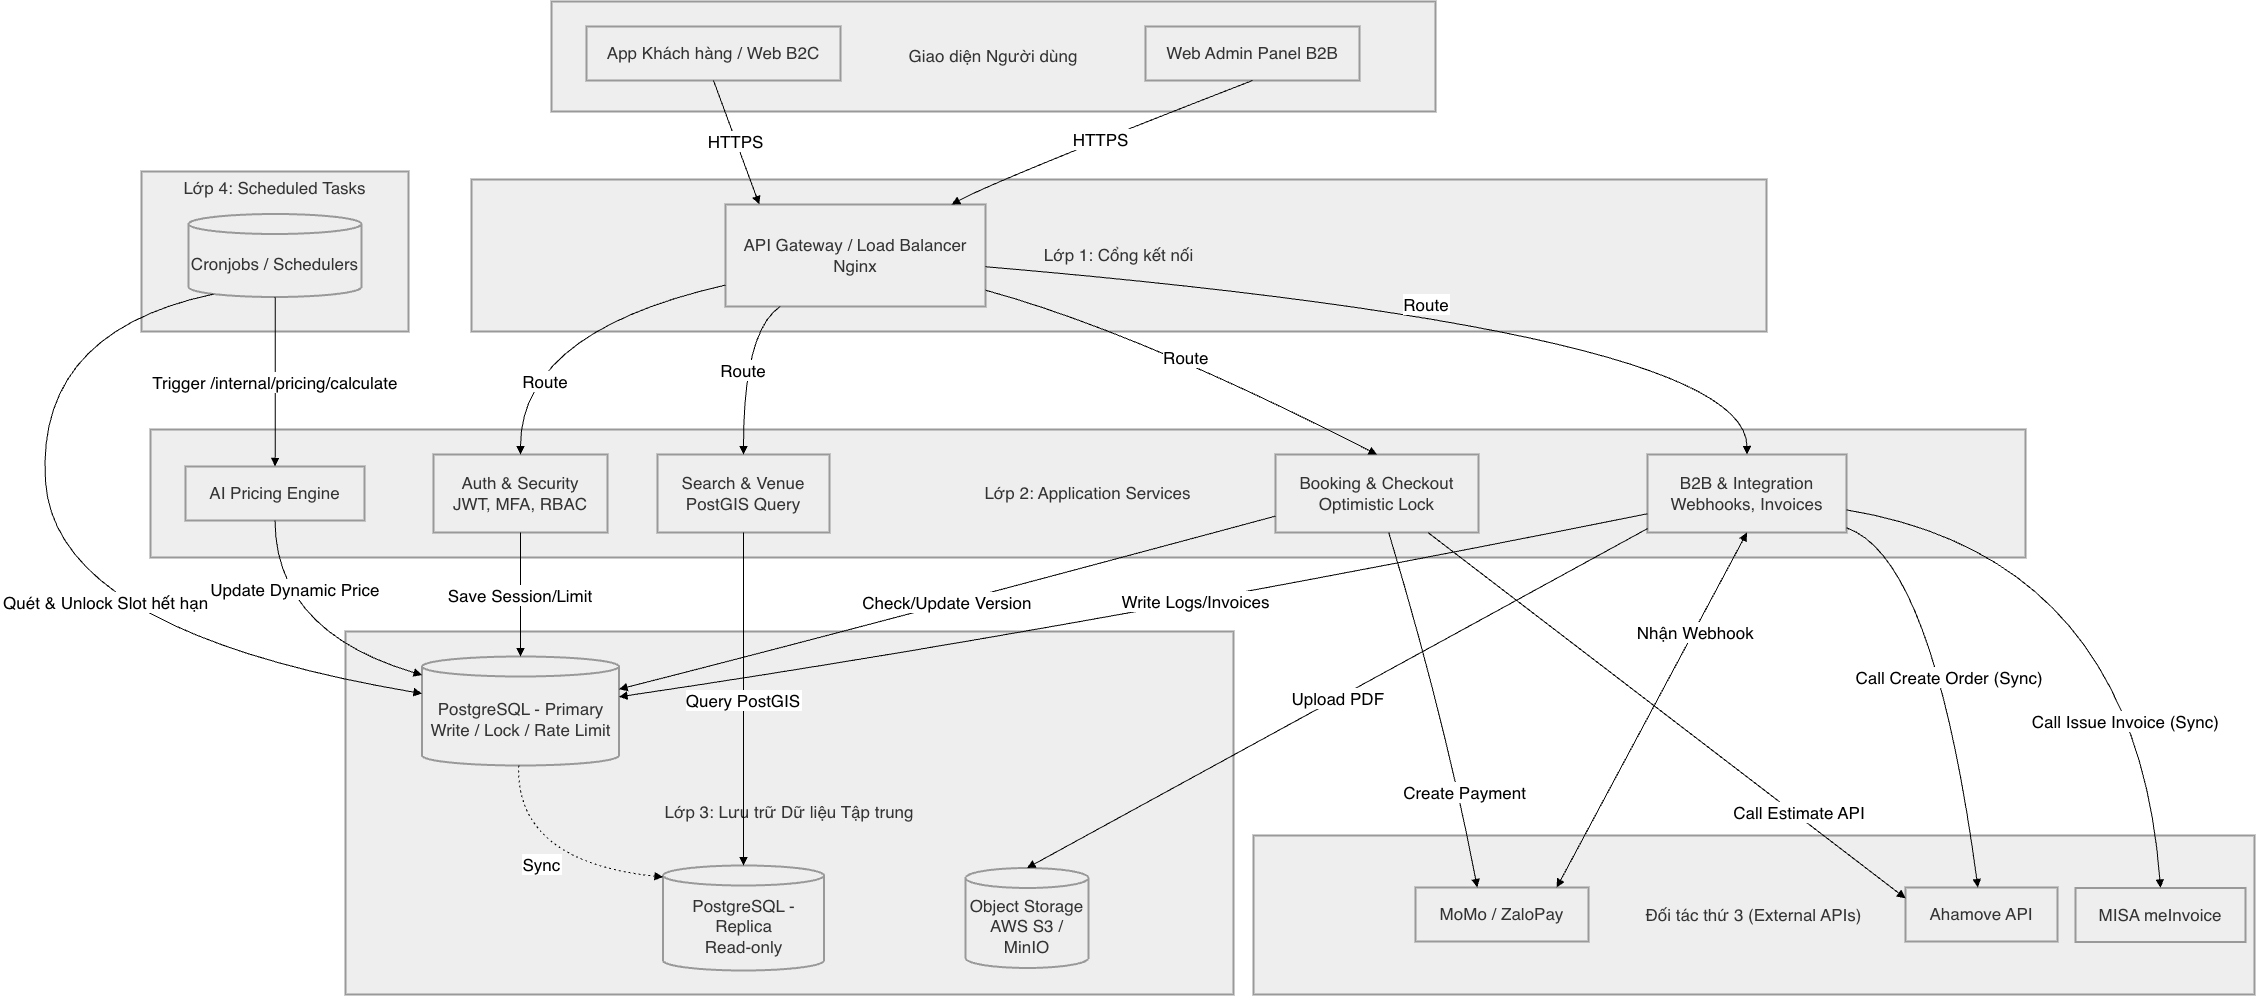
\includegraphics[width=1\textwidth]{Images/TMĐT_252-system.drawio.png}
    \caption{Sơ đồ kiến trúc hạ tầng tổng thể của hệ thống CourtMate}
    \label{fig:simplified_arch}
\end{figure}

Hình \ref{fig:simplified_arch} minh họa kiến trúc hạ tầng tổng thể của hệ thống CourtMate. Hệ thống được tổ chức thành các lớp (Layers) tách biệt nhằm đảm bảo tính linh hoạt và dễ quản lý. Kiến trúc này được lựa chọn nhằm ưu tiên tính khả thi, chi phí thấp và khả năng mở rộng tuyến tính cho giai đoạn MVP của hệ thống.

\subsection{Chi tiết các lớp kiến trúc phân tầng}

\subsubsection{Lớp Biên (Edge Layer - Lớp 1: Cổng kết nối)}
\begin{itemize}
    \item \textbf{Thành phần:} Nginx (đóng vai trò API Gateway và Load Balancer).
    \item \textbf{Nhiệm vụ:} Đây là điểm tiếp nhận duy nhất cho toàn bộ lưu lượng HTTPS từ App Khách hàng / Web B2C và Web Admin Panel B2B. Nginx chịu trách nhiệm phân giải (Routing) dựa trên đường dẫn URL để đưa request đến đúng cụm dịch vụ bên dưới một cách minh bạch.
\end{itemize}

\subsubsection{Lớp Ứng dụng (Application Layer - Lớp 2)}
Áp dụng chiến lược lập trình đa ngôn ngữ (Polyglot Programming), tách các module thành các service độc lập để dễ dàng mở rộng:
\begin{itemize}
    \item \textbf{Auth \& Security (JWT, MFA, RBAC):} Đứng trước các service nghiệp vụ để xác thực danh tính người dùng và phân quyền truy cập.
    \item \textbf{Search \& Venue (Node.js/Express):} Xử lý các truy vấn tìm kiếm sân bãi thông qua PostGIS, ưu tiên tốc độ I/O bất đồng bộ để đáp ứng lượng request khổng lồ.
    \item \textbf{Booking \& Checkout (Node.js/Express):} Xử lý luồng đặt sân hướng khách hàng, quản lý vòng đời đơn hàng và cơ chế giữ chỗ (Optimistic Lock).
    \item \textbf{B2B \& Integration (Java/Spring Boot 3.2):} Xử lý các tính năng quản trị phức tạp của chủ sân và giao tiếp đồng bộ (Sync) với các đối tác thứ ba (MISA meInvoice). Java Spring Boot đảm bảo tính chặt chẽ, toàn vẹn giao dịch (ACID).
    \item \textbf{AI Pricing Engine (Python/FastAPI):} Cô lập hoàn toàn logic tính toán Machine Learning nặng nề. Được kích hoạt bởi Cronjobs/Schedulers (Lớp 4), AI Engine sẽ tính toán giá mới và cập nhật thẳng xuống cơ sở dữ liệu mà không làm nghẽn luồng xử lý web chính.
\end{itemize}

\subsubsection{Lớp Dữ liệu (Data Layer - Lớp 3: Lưu trữ Dữ liệu Tập trung)}
Hệ thống áp dụng mẫu thiết kế Shared Database Pattern (Dùng chung cơ sở dữ liệu) được tối ưu hóa:
\begin{itemize}
    \item \textbf{PostgreSQL (Primary):} Xử lý các luồng thao tác Ghi (Write), Khóa (Lock), và Giới hạn tỷ lệ (Rate Limit).
    \item \textbf{PostgreSQL (Replica - Read-only):} Được đồng bộ hóa từ cụm Primary. Kết hợp với PostGIS để chuyên biệt hóa cho các truy vấn Đọc (Read) và tìm kiếm không gian địa lý, giúp giảm tải tối đa cho cơ sở dữ liệu chính.
    \item \textbf{Object Storage (AWS S3 / MinIO):} Lưu trữ tài nguyên phi cấu trúc, tệp tĩnh như hình ảnh, file hóa đơn PDF.
\end{itemize}

\subsubsection{Lớp Hạ tầng và Đối tác (Infrastructure \& External APIs)}
Hệ thống kết hợp sức mạnh của Multi-Cloud:
\begin{itemize}
    \item Máy chủ tính toán đặt tại Việt Nam (như Bizfly/Viettel Cloud) để đạt độ trễ mạng cực thấp.
    \item Tích hợp sâu vào các Webhook/API ngoại vi: VietQR (Dòng tiền tài chính), MISA (Hóa đơn điện tử).
\end{itemize}

\newpage
\section{Thiết kế, Hiện thực và Đánh giá}
\subsection{Công nghệ triển khai (Tech Stack)}
Nhằm phát huy tối đa thế mạnh của các thành viên trong nhóm và tính chất của từng dịch vụ, CourtMate được triển khai trên nền tảng công nghệ đa ngôn ngữ (Polyglot Programming):

\begin{itemize}
    \item \textbf{Frontend Application:} Sử dụng Next.js 14 (App Router) kết hợp cùng TailwindCSS, mang lại tốc độ phản hồi nhanh (Server-side Rendering) và giao diện chuẩn UI/UX hiện đại.    \item \textbf{B2C Booking Service:} Xây dựng trên nền tảng Node.js và Express, sử dụng Prisma ORM để tương tác với cơ sở dữ liệu, giúp xử lý các request đặt sân từ người chơi một cách linh hoạt.    \item \textbf{B2B Admin Service:} Sử dụng Java 17 và Spring Boot 3.2 kết hợp cùng Spring Data JPA, đảm bảo tính chặt chẽ và ổn định cho các nghiệp vụ quản lý doanh thu, sân bãi của đối tác.    \item \textbf{AI Pricing Engine:} Triển khai bằng ngôn ngữ Python thông qua framework FastAPI, tận dụng sức mạnh của các thư viện xử lý dữ liệu và máy học chuyên sâu.    \item \textbf{API Documentation:} Sử dụng Swagger/OpenAPI 3.0 để chuẩn hóa tài liệu giao tiếp giữa các dịch vụ B2C, B2B và mã nguồn Frontend.\end{itemize}

\subsection{Đặc tả Giao diện và Trải nghiệm Người dùng (UI/UX)}

Hệ thống CourtMate được thiết kế không chỉ nhằm đáp ứng toàn diện các yêu cầu chức năng mà còn đặc biệt chú trọng đến việc tối ưu hóa trải nghiệm người dùng (User Experience - UX) và củng cố bộ nhận diện thương hiệu (Brand Identity). Các quyết định thiết kế cốt lõi được định hình dựa trên quá trình phân tích chuyên sâu về mô hình kinh doanh kết hợp cùng các nguyên tắc thiết kế tương tác chuẩn mực.

\subsubsection{Hệ thống Nhận diện Thương hiệu (Brand Identity)}
\begin{itemize}
    \item \textbf{Màu sắc chủ đạo (Color Palette):} Sử dụng Xanh Hoàng gia (Royal Blue - \#1D4ED8) làm tông màu nhận diện cốt lõi. Sắc xanh này không chỉ truyền tải sự năng động, tinh thần thể thao mà còn khẳng định độ tin cậy của một nền tảng công nghệ thanh toán. Các gam màu phụ trợ như Trắng (\#FFFFFF) và Xám nhạt (\#F8FAFC) được vận dụng linh hoạt làm màu nền, tạo không gian trắng (\textit{white space}) tối ưu nhằm làm nổi bật luồng thông tin trọng tâm.
    \item \textbf{Ngôn ngữ hình khối và Nghệ thuật chữ (Shapes \& Typography):} Áp dụng nhất quán ngôn ngữ thiết kế bo góc (\texttt{border-radius} 16px-24px) đối với các thành phần giao diện như thẻ (cards), nút bấm (buttons) và khối thời gian (slots) dưới dạng viên thuốc (pill-shaped). Lối tiếp cận này mang lại cảm giác thân thiện, hiện đại, đồng thời phá vỡ sự cứng nhắc thường thấy ở các hệ thống quản trị truyền thống. Hệ phông chữ Sans-serif hiện đại được triển khai xuyên suốt, kết hợp với các trọng số (\texttt{font-weight}) in đậm nhằm tạo điểm nhấn thị giác cho các chỉ số KPI và dữ liệu quan trọng.
\end{itemize}

\subsubsection{Thiết kế UI/UX bám sát Mô hình Kinh doanh (Business Model Alignment)}
\begin{itemize}
    \item \textbf{Đối với phân hệ B2C (Người chơi):} Tiêu chí cốt lõi là tốc độ và sự tiện lợi ("Đặt sân trong 30 giây"). Giao diện được kiến trúc theo triết lý Mobile-first, tinh gọn quy trình thanh toán (Checkout) thành 3 bước tuyến tính. Các tính năng như sảnh chờ ghép trận (Matchmaking Lobby - ứng dụng biểu đồ Radar Chart để trực quan hóa năng lực) và vé điện tử (QR Ticket) được thiết kế hiện đại, đề cao tính tương tác xã hội, đáp ứng chính xác thị hiếu của tệp khách hàng Gen Z.
    \item \textbf{Đối với phân hệ B2B (Chủ sân):} Trọng tâm thiết kế hướng đến năng lực kiểm soát toàn diện và tối ưu hóa hiệu suất vận hành. Giao diện Admin Panel cung cấp khối lượng dữ liệu lớn nhưng triệt tiêu hiện tượng quá tải nhận thức nhờ bố cục phân mảnh (Split-view). Lưới thời gian tương tác (Interactive Slot Grid) số hóa hoàn toàn sổ đặt sân truyền thống, tích hợp thao tác kéo-thả (Drag-and-drop) trực quan, qua đó thúc đẩy quá trình chuyển đổi số diễn ra tự nhiên và xóa bỏ rào cản thao tác cho chủ cơ sở.
\end{itemize}

\subsubsection{Các Nguyên tắc Thiết kế (Design Principles) Ứng dụng}
\begin{itemize}
    \item \textbf{Tính Nhất quán (Consistency):} Cả hai phân hệ B2C và B2B đều tuân thủ nghiêm ngặt một Hệ thống thiết kế (Design System) chung, đồng nhất về bảng màu, hiệu ứng thị giác (drop-shadow) và quy chuẩn bo góc. Điều này kiến tạo nên một hệ sinh thái CourtMate liền mạch và chuyên nghiệp.
    \item \textbf{Định luật Hick (Hick's Law):} Nhằm tối ưu hóa thời gian ra quyết định của người dùng, hệ thống chủ động ẩn các bộ lọc phức tạp tại màn hình chính, ưu tiên hiển thị thanh "Tìm kiếm nhanh" và phân nhóm hợp lý các luồng thanh toán để tránh gây nhiễu loạn thông tin.
    \item \textbf{Phân cấp thị giác (Visual Hierarchy):} Các nút Kêu gọi hành động (Call-to-Action) trọng yếu như "Book Now" hay "Join \& Split Payment" luôn được thiết lập màu xanh chủ đạo với độ tương phản cao nhất. Ngược lại, các thông tin thứ yếu được làm dịu bằng tông màu xám nhằm điều hướng sự tập trung.
    \item \textbf{Tính chi trả (Affordance) và Phản hồi (Feedback):} Trên giao diện lưới lịch quản trị, các suất chơi trống được biểu thị bằng viền nét đứt, ngầm định khả năng tương tác. Đồng thời, hệ thống mã hóa màu sắc (Xanh = Đã xác nhận, Vàng = Đang chờ, Đỏ = Lỗi) cung cấp phản hồi thị giác tức thời và minh bạch khi hệ thống xử lý các tác vụ nền (như gọi AI Engine hay đồng bộ ERP MISA).
\end{itemize}
\vspace{0.5cm}
\noindent\textbf{Đặc tả kỹ thuật và luồng trải nghiệm người dùng (UX Flow) cho các màn hình cốt lõi:}

\begin{enumerate}
    \item \textbf{Luồng Onboarding: Xác thực và Định danh} \textit{(Bao gồm 2 màn hình: Đăng ký, Đăng nhập)}
    \begin{itemize}
        \item \textit{Layout:} Giao diện Split-view tối ưu hóa không gian, kết hợp hình ảnh mang tinh thần thể thao trực quan và form nhập liệu tập trung.
        \item \textit{Components:} Bộ phân loại đối tượng người dùng (Nút switch: "Tôi là Người chơi" / "Tôi là Chủ sân"); Tích hợp Đăng nhập một chạm qua mạng xã hội (Google, Facebook) giảm thiểu rào cản tham gia; Nút biểu tượng mắt để ẩn/hiện mật khẩu.
        \item \textit{Flow:} Truy cập ứng dụng $\rightarrow$ Chọn phân hệ B2C hoặc B2B ngay từ màn hình đầu tiên $\rightarrow$ Nhập thông tin (Họ tên, SĐT, Email) $\rightarrow$ Xác thực thành công và điều hướng về Homepage (B2C) hoặc Dashboard (B2B).
    \end{itemize}
    \begin{figure}[h!]
        \centering
        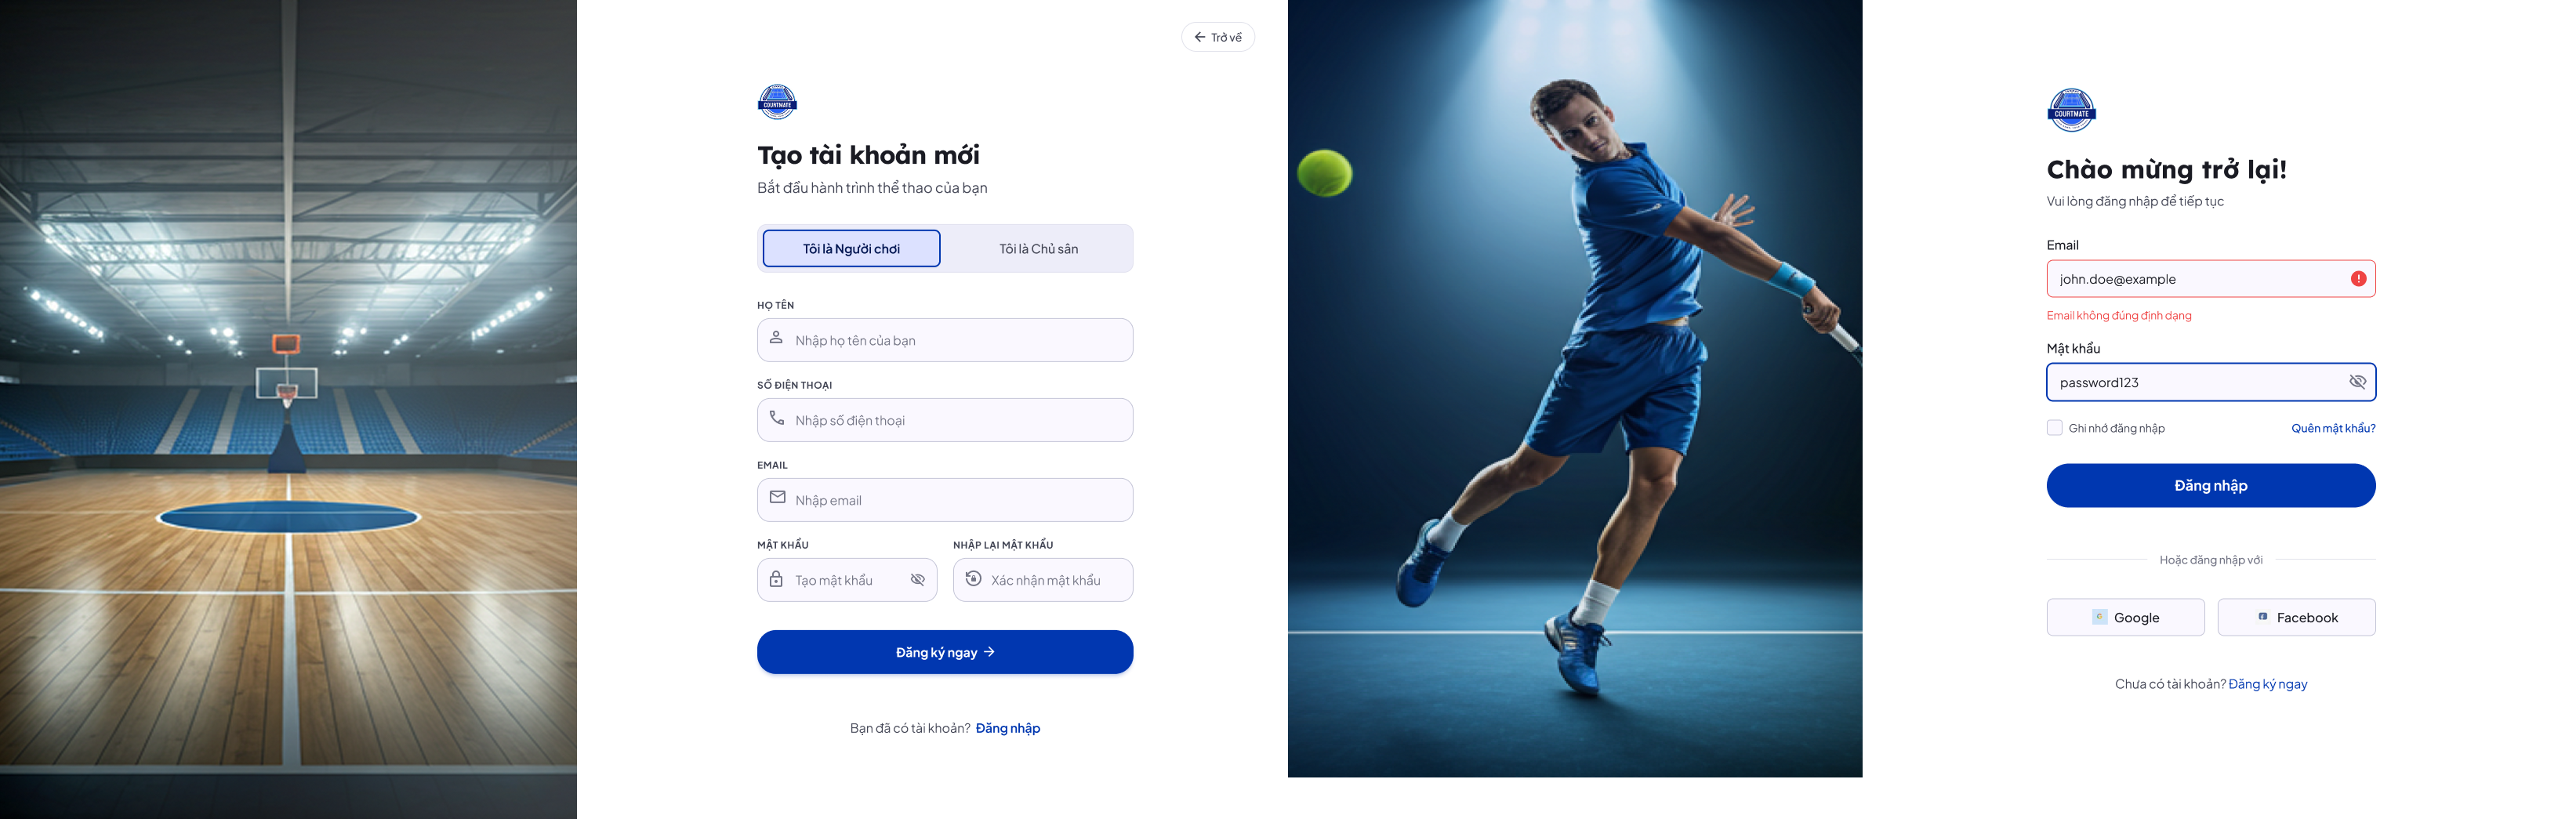
\includegraphics[width=0.8\linewidth]{Images/hinh_01_onboarding.png}
        \caption{Giao diện Xác thực và Định danh, phân loại rõ luồng đăng ký/đăng nhập dành cho Người chơi và Chủ sân.}
        \label{fig:onboarding}
    \end{figure}

    \item \textbf{Luồng Khám phá và Tìm kiếm sân (Spatial Search \& Discovery)} \textit{(Bao gồm 3 màn hình: Trang chủ, Tìm kiếm Bản đồ, Chi tiết Sân)}
    \begin{itemize}
        \item \textit{Layout:} Tích hợp bộ tìm kiếm nhanh tại Trang chủ và Trang Khám phá dạng Split-view (Bản đồ Mapbox chiếm 60\% diện tích màn hình).
        \item \textit{Components:} Bộ lọc đa tầng (Địa điểm, Môn thể thao: Pickleball/Tennis/Cầu lông, Ngày); Thẻ chi tiết sân hiển thị tiện ích (Free Wifi, Parking, Canteen), Điểm đánh giá (Rating) và Review thực tế từ người dùng.
        \item \textit{Flow:} Tìm kiếm tại màn hình chính $\rightarrow$ Chuyển sang giao diện Bản đồ, tương tác kéo thả $\rightarrow$ Gửi tọa độ Hộp giới hạn (Bounding Box) về Backend $\rightarrow$ Hiển thị danh sách sân $\rightarrow$ Nhấp chọn Sân Pickleball/Tennis để xem chi tiết $\rightarrow$ Chọn khung giờ (Slot) khả dụng $\rightarrow$ Nhấn "Book Now".
    \end{itemize}
    \begin{figure}[h!]
        \centering
        \includegraphics[width=\linewidth]{Images/hinh_02_kham_pha_san.png}
        \caption{Giao diện Trang chủ, Tìm kiếm không gian địa lý (Spatial Search) và Chi tiết cụm sân với lưới chọn slot theo thời gian thực.}
        \label{fig:kham_pha}
    \end{figure}

    \item \textbf{Luồng Giao dịch \& Thanh toán (Transaction \& Checkout Pipeline)} \textit{(Bao gồm 6 màn hình: Review 1, Payment Modal, Thẻ tín dụng, Quét QR SePay, Confirm 3, Layout chờ)}
    \begin{itemize}
        \item \textit{Layout:} Quy trình Checkout 3 bước tuyến tính rõ ràng (1. Review $\rightarrow$ 2. Payment $\rightarrow$ 3. Confirm).
        \item \textit{Components:} Bảng tóm tắt thông tin đặt sân kèm chính sách hủy sân (hoàn tiền 100\% trước 24h); Modal pop-up chọn phương thức thanh toán (Credit Card, MoMo, SePay QR); Dynamic QR Generator.
        \item \textit{Flow:} Nhấn "Đặt ngay" tại chi tiết sân $\rightarrow$ Backend kích hoạt Optimistic Lock (\texttt{locked\_until}) $\rightarrow$ Chuyển sang bước Review (kiểm tra ngày, giờ, tiền sân) $\rightarrow$ Chọn hình thức (Thẻ/Ví điện tử/VietQR) $\rightarrow$ Quét mã/Nhập thông tin thẻ $\rightarrow$ Webhook báo thành công $\rightarrow$ Chuyển sang màn hình Booking Confirmed.
    \end{itemize}
    \begin{figure}[h!]
        \centering
        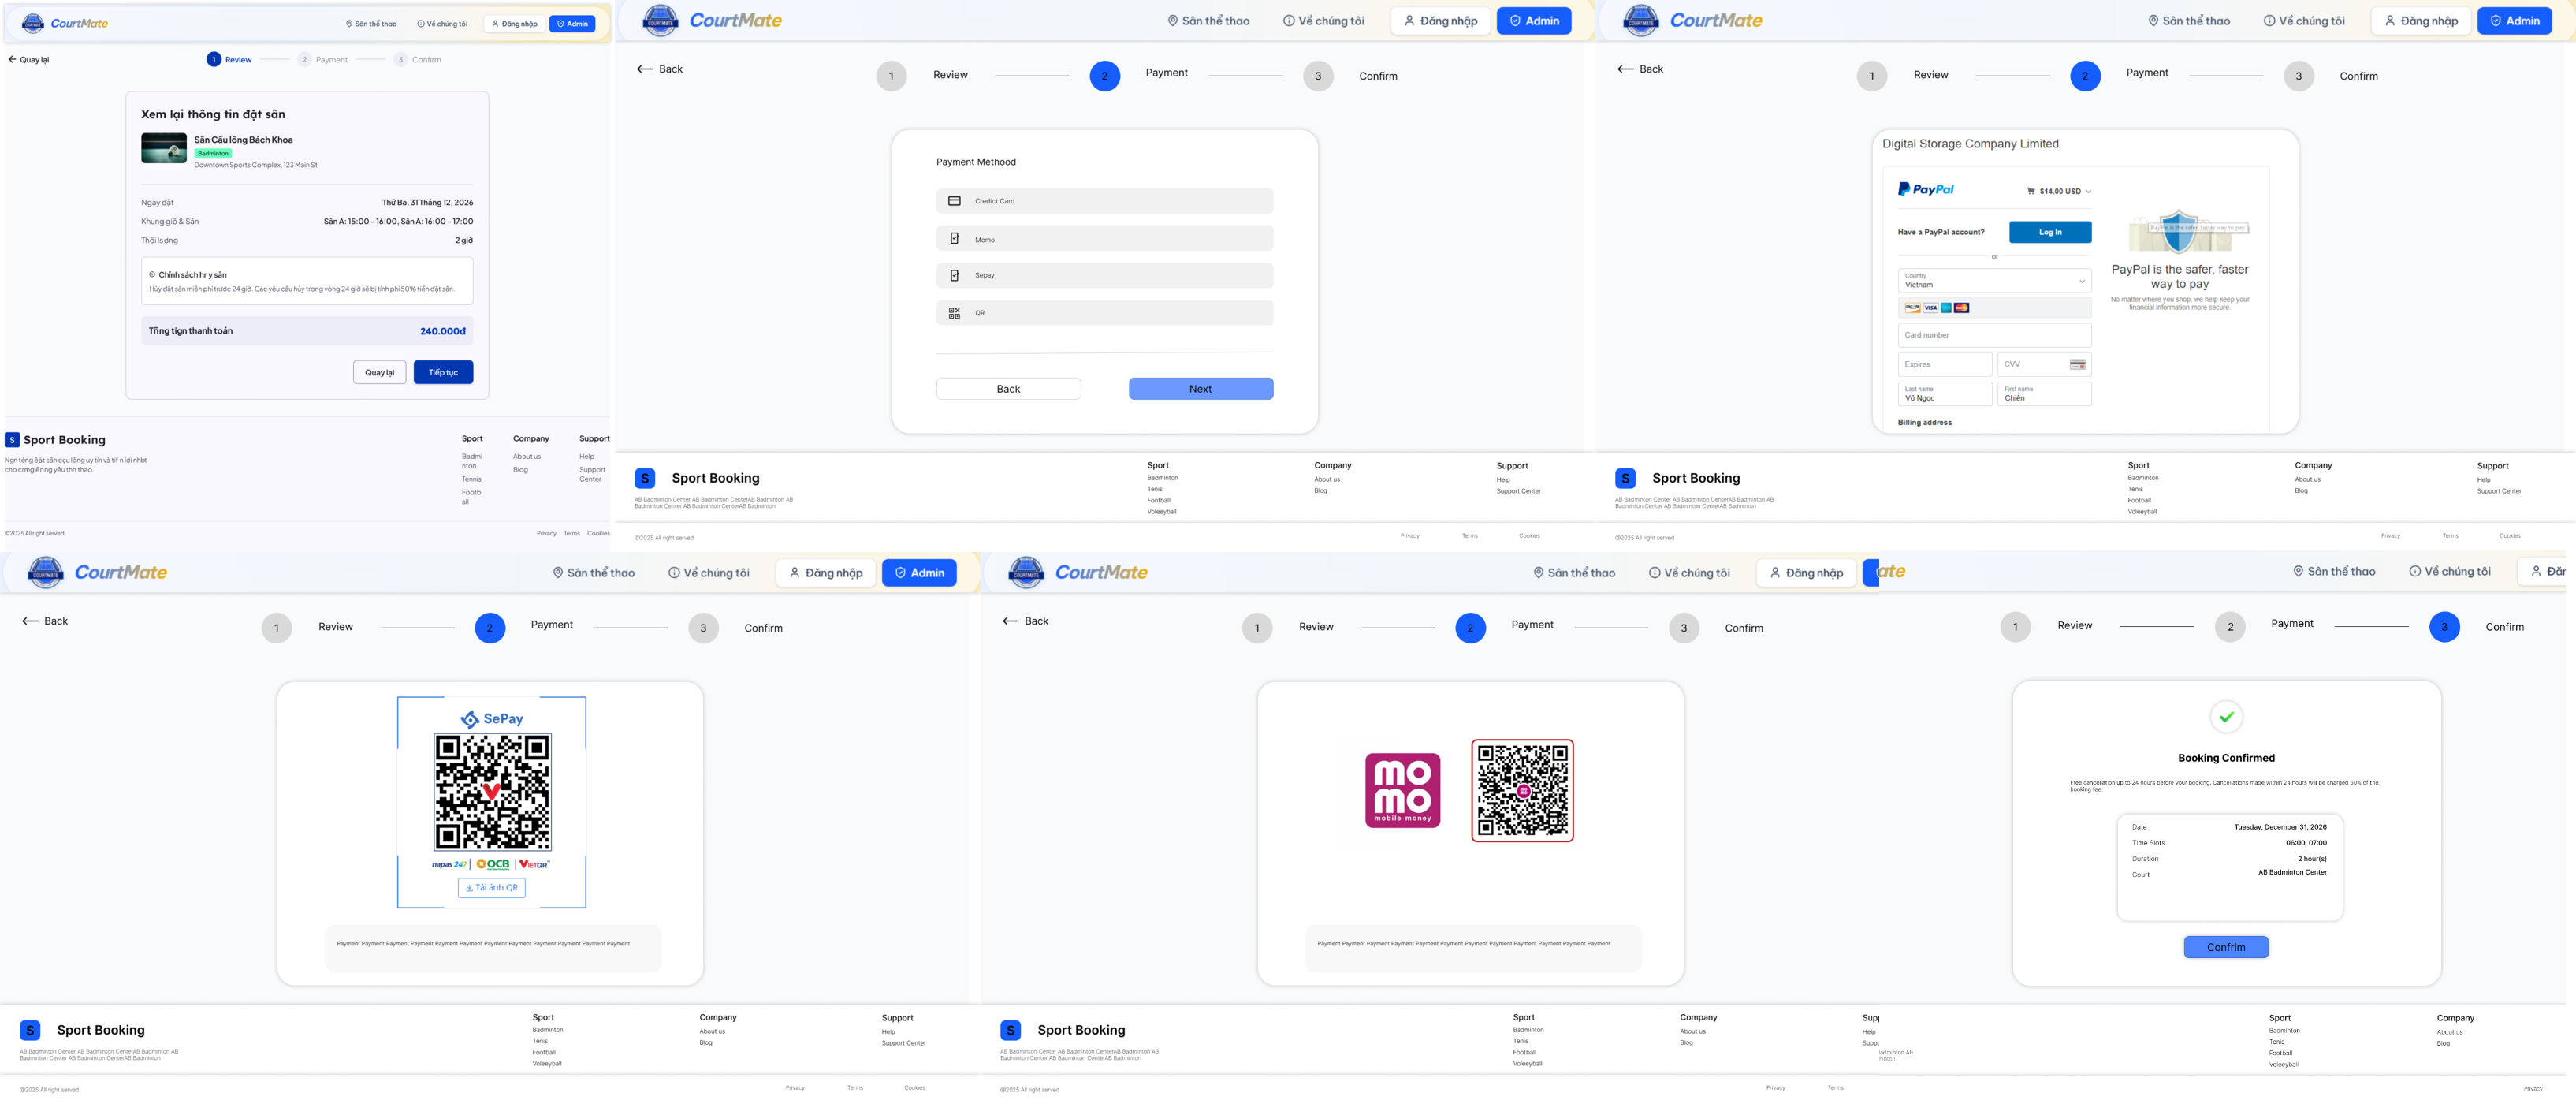
\includegraphics[width=\linewidth]{Images/hinh_03_thanh_toan_checkout.png}
        \caption{Quy trình Checkout 3 bước tuyến tính, hỗ trợ đa dạng phương thức thanh toán (Credit Card, PayPal, MoMo, VietQR).}
        \label{fig:thanh_toan}
    \end{figure}

    \item \textbf{Luồng Quản lý Lịch sử Đặt sân (Player Booking Management)} \textit{(Bao gồm 2 màn hình: Danh sách Lịch sử, Chi tiết Đơn đặt)}
    \begin{itemize}
        \item \textit{Layout:} Giao diện quản lý cá nhân với hệ thống phân trang/Tab theo trạng thái: Sắp tới, Đã chơi, Đã hủy.
        \item \textit{Components:} Thẻ trạng thái đơn hàng trực quan; Giao diện bóc tách chi tiết mã đơn (Tiền sân, Phí dịch vụ, Giảm giá); Nút hành động (Call-to-Action) để Hủy slot/Thanh toán ngay.
        \item \textit{Flow:} Truy cập Lịch sử đặt sân $\rightarrow$ Xem tổng quan các đơn $\rightarrow$ Nhấp vào đơn (VD: \#CM-12345) $\rightarrow$ Kiểm tra danh sách các Slot đã đặt $\rightarrow$ Thực hiện Hủy slot (nếu chưa vi phạm mốc thời gian quy định).
    \end{itemize}
    \begin{figure}[h!]
        \centering
        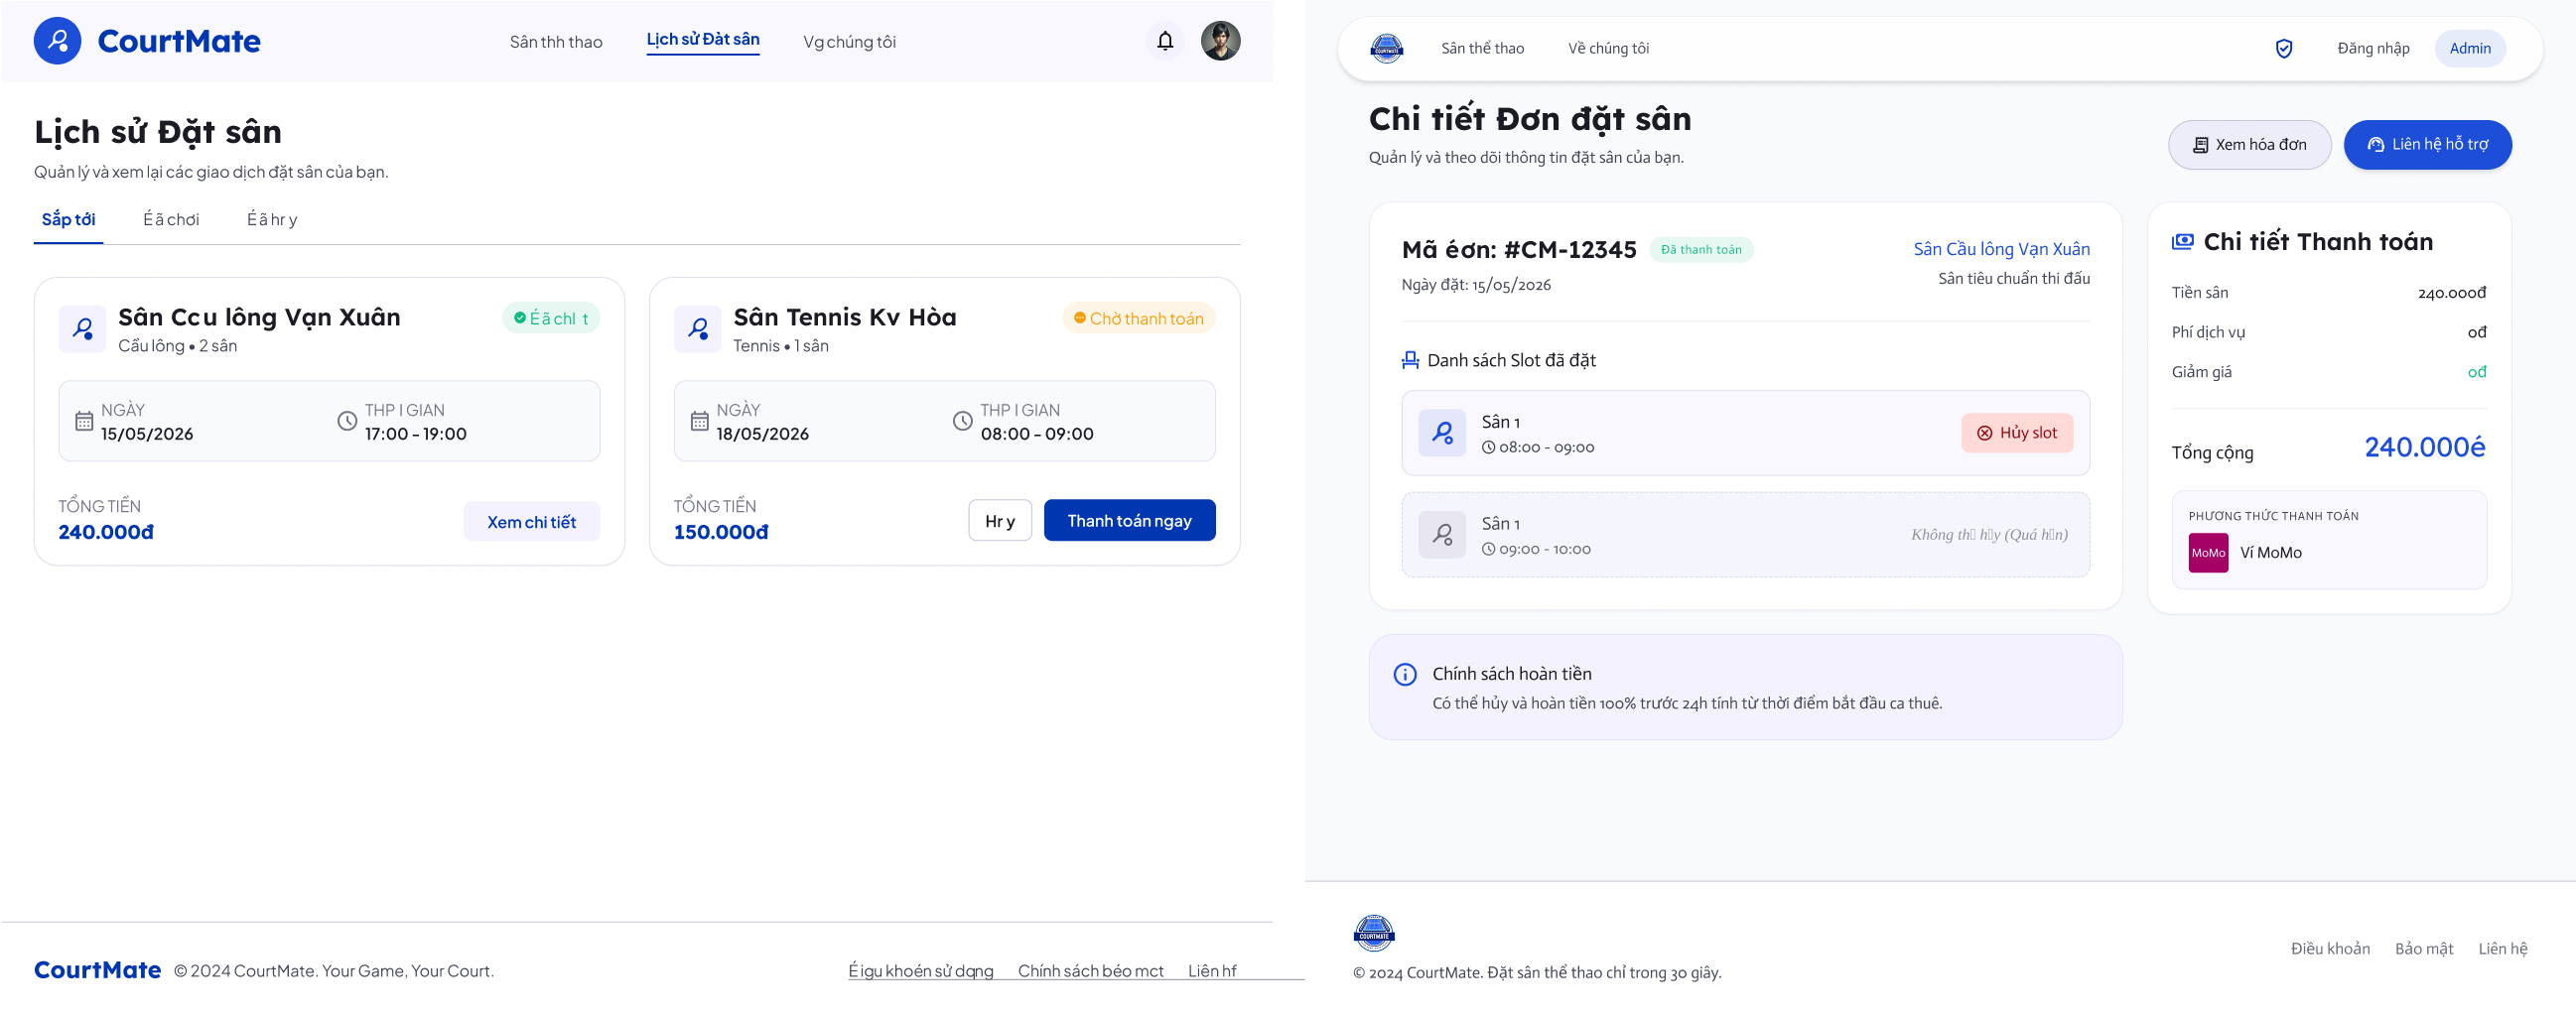
\includegraphics[width=0.8\linewidth]{Images/hinh_04_lich_su_dat_san.png}
        \caption{Giao diện Quản lý Lịch sử Đặt sân và Chi tiết Đơn hàng cá nhân dành cho Người chơi.}
        \label{fig:lich_su}
    \end{figure}

    \item \textbf{Admin Operational Dashboard \& Heatmap} \textit{(Bao gồm 1 màn hình: Tổng quan Dashboard)}
    \begin{itemize}
        \item \textit{Layout:} Cấu trúc chuẩn với thanh điều hướng (Sidebar) bên trái và vùng làm việc (Main Panel) bên phải trình bày các Widget.
        \item \textit{Components:} Thẻ chỉ số tổng quan (Total Revenue, Total Bookings, Utilization Rate); Biểu đồ lưới nhiệt (Court Occupancy Heatmap) ứng dụng \texttt{Recharts} để trực quan hóa mức lấp đầy (0\% - 100\%) theo từng khung giờ trong tuần.
        \item \textit{Flow:} Đăng nhập tài khoản B2B $\rightarrow$ Dữ liệu tổng hợp Real-time hiển thị lên Dashboard $\rightarrow$ Admin rà chuột (Hover) qua các ô của Heatmap để xem tỷ lệ lấp đầy chi tiết của từng giờ.
    \end{itemize}
    \begin{figure}[h!]
        \centering
        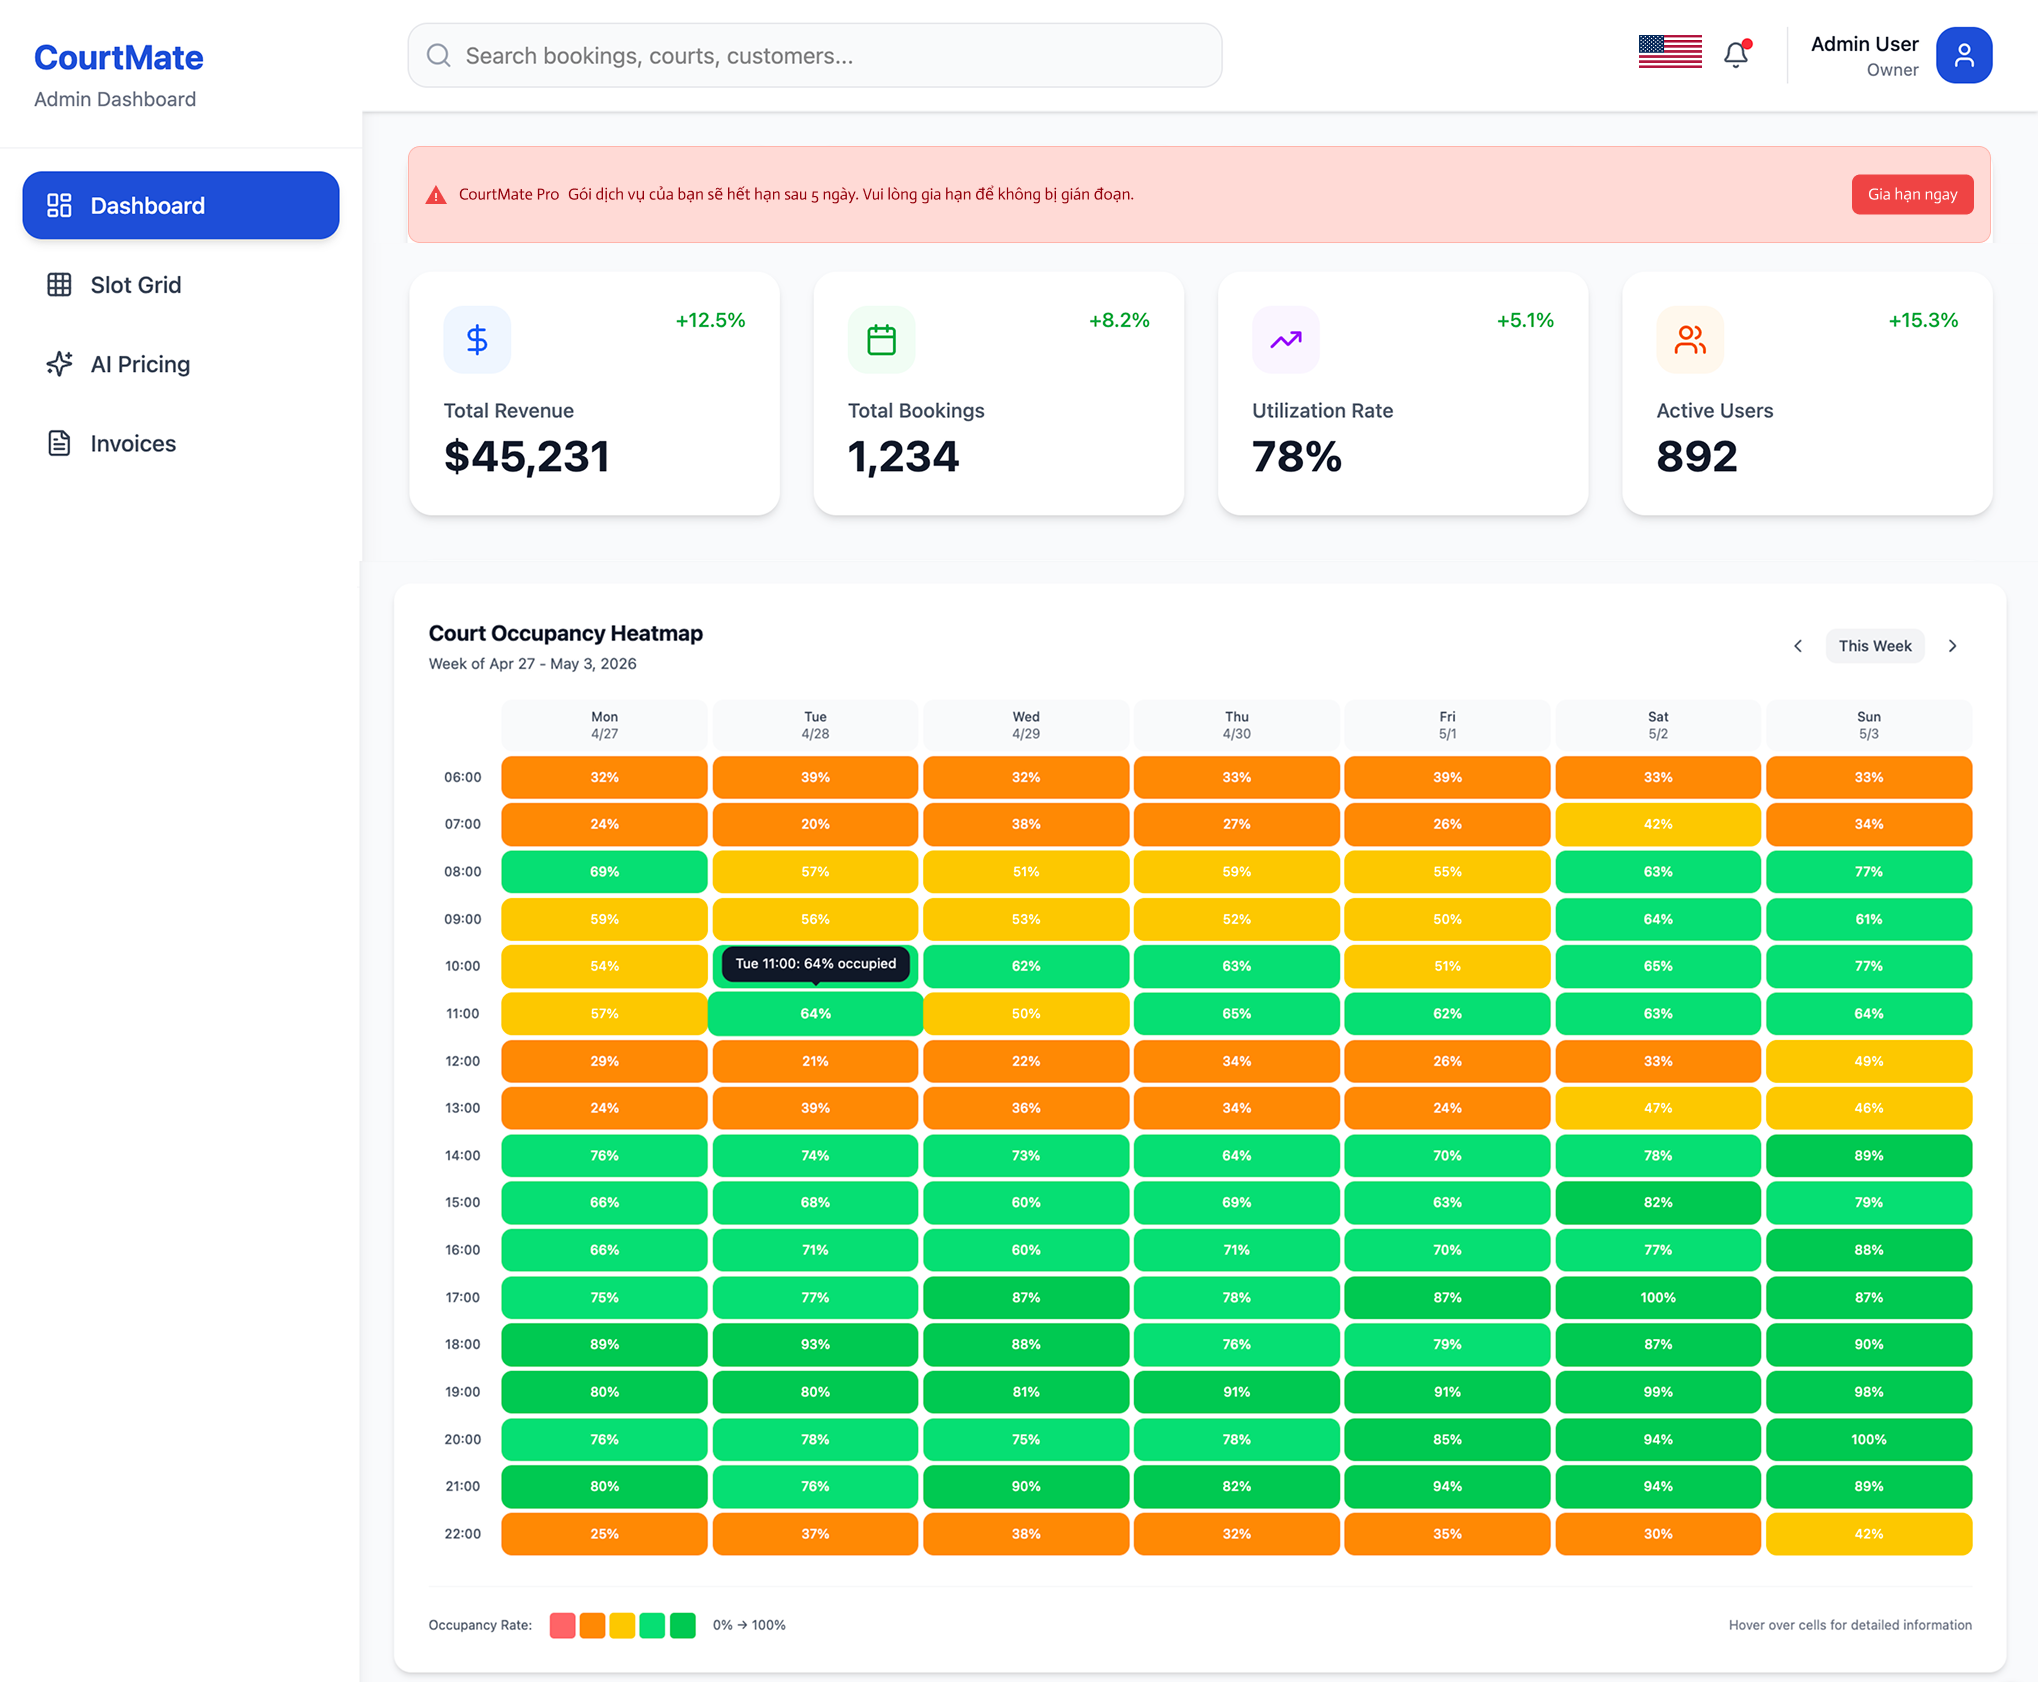
\includegraphics[width=\linewidth]{Images/hinh_05_admin_dashboard.png}
        \caption{Bảng điều khiển Vận hành B2B với hệ thống thẻ chỉ số tổng quan và Biểu đồ nhiệt (Heatmap) lấp đầy.}
        \label{fig:admin_dashboard}
    \end{figure}

    \item \textbf{Interactive Slot Grid (Quản lý suất chơi thời gian thực)} \textit{(Bao gồm 1 màn hình: Lưới lịch)}
    \begin{itemize}
        \item \textit{Layout:} Dạng ma trận với Trục tung (thời gian) và Trục hoành (danh sách sân bãi).
        \item \textit{Components:} Lưới thao tác kéo-thả (\texttt{dnd-kit}); Hệ thống mã hóa màu sắc (Xanh: Đã đặt, Vàng: Chờ xử lý, Trắng: Trống).
        \item \textit{Flow:} Admin chọn khung giờ bị khuyết $\rightarrow$ Hiển thị pop-up tạo Booking thủ công $\rightarrow$ Hoặc kéo-thả slot để dời lịch cho khách hàng $\rightarrow$ Hệ thống gọi API đồng bộ trạng thái toàn cục.
    \end{itemize}
    \begin{figure}[h!]
        \centering
        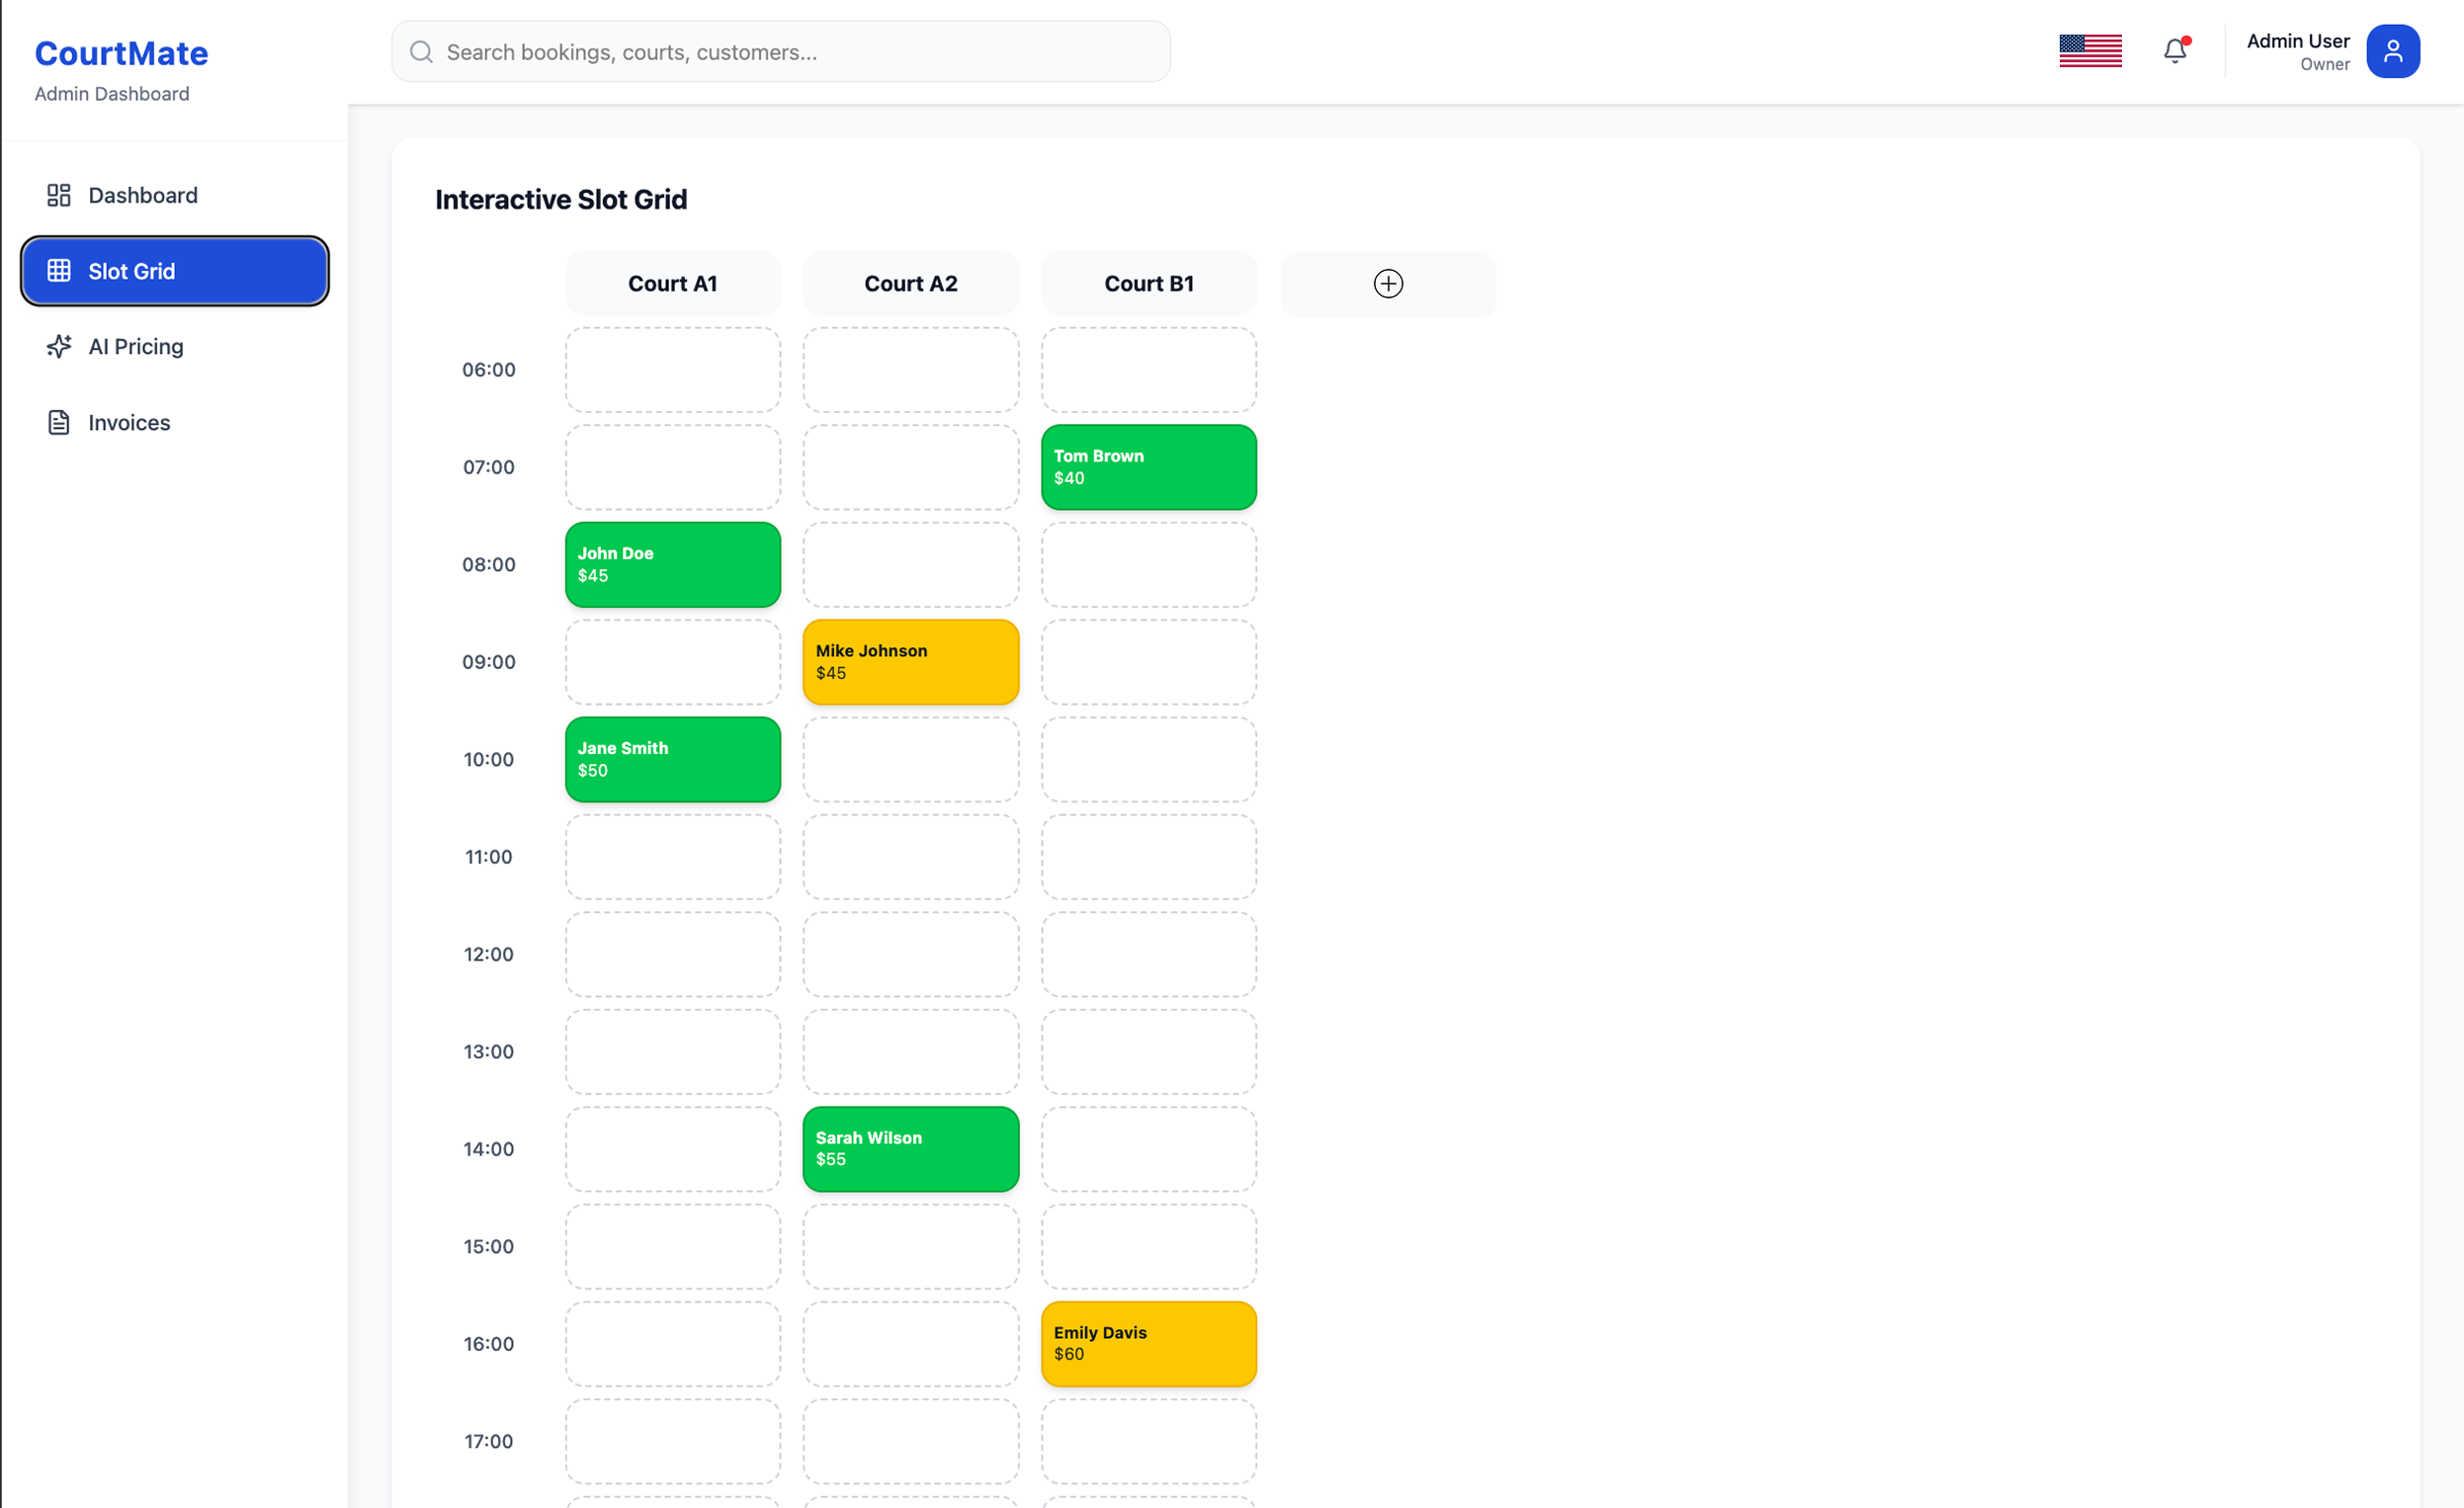
\includegraphics[width=\linewidth]{Images/hinh_06_slot_grid.png}
        \caption{Lưới lịch tương tác (Interactive Slot Grid) cho phép Chủ sân bao quát và quản lý các ca trực trực tiếp.}
        \label{fig:slot_grid}
    \end{figure}

    \item \textbf{AI Pricing Configurator (Cấu hình Định giá AI)} \textit{(Bao gồm 1 màn hình: Thiết lập AI Pricing)}
    \begin{itemize}
        \item \textit{Layout:} Giao diện cấu hình chia đôi: Form nhập liệu (trái) và Biểu đồ dự báo (phải).
        \item \textit{Components:} Trường thiết lập (Giá cơ sở, Giá sàn, Giá trần); Thanh trượt (Slider) giới hạn tỷ lệ lấp đầy; Tùy chọn chiến lược tối ưu (Max Revenue / Max Occupancy); Biểu đồ Projected Price Trend.
        \item \textit{Flow:} Nhập tham số an toàn $\rightarrow$ Xem trước đồ thị dự báo biến thiên giá theo giờ $\rightarrow$ Bật công tắc (Toggle) "Tự động điều chỉnh giá" $\rightarrow$ AI Engine lưu cấu hình và tự động kích hoạt Yield Management.
    \end{itemize}
    \begin{figure}[h!]
        \centering
        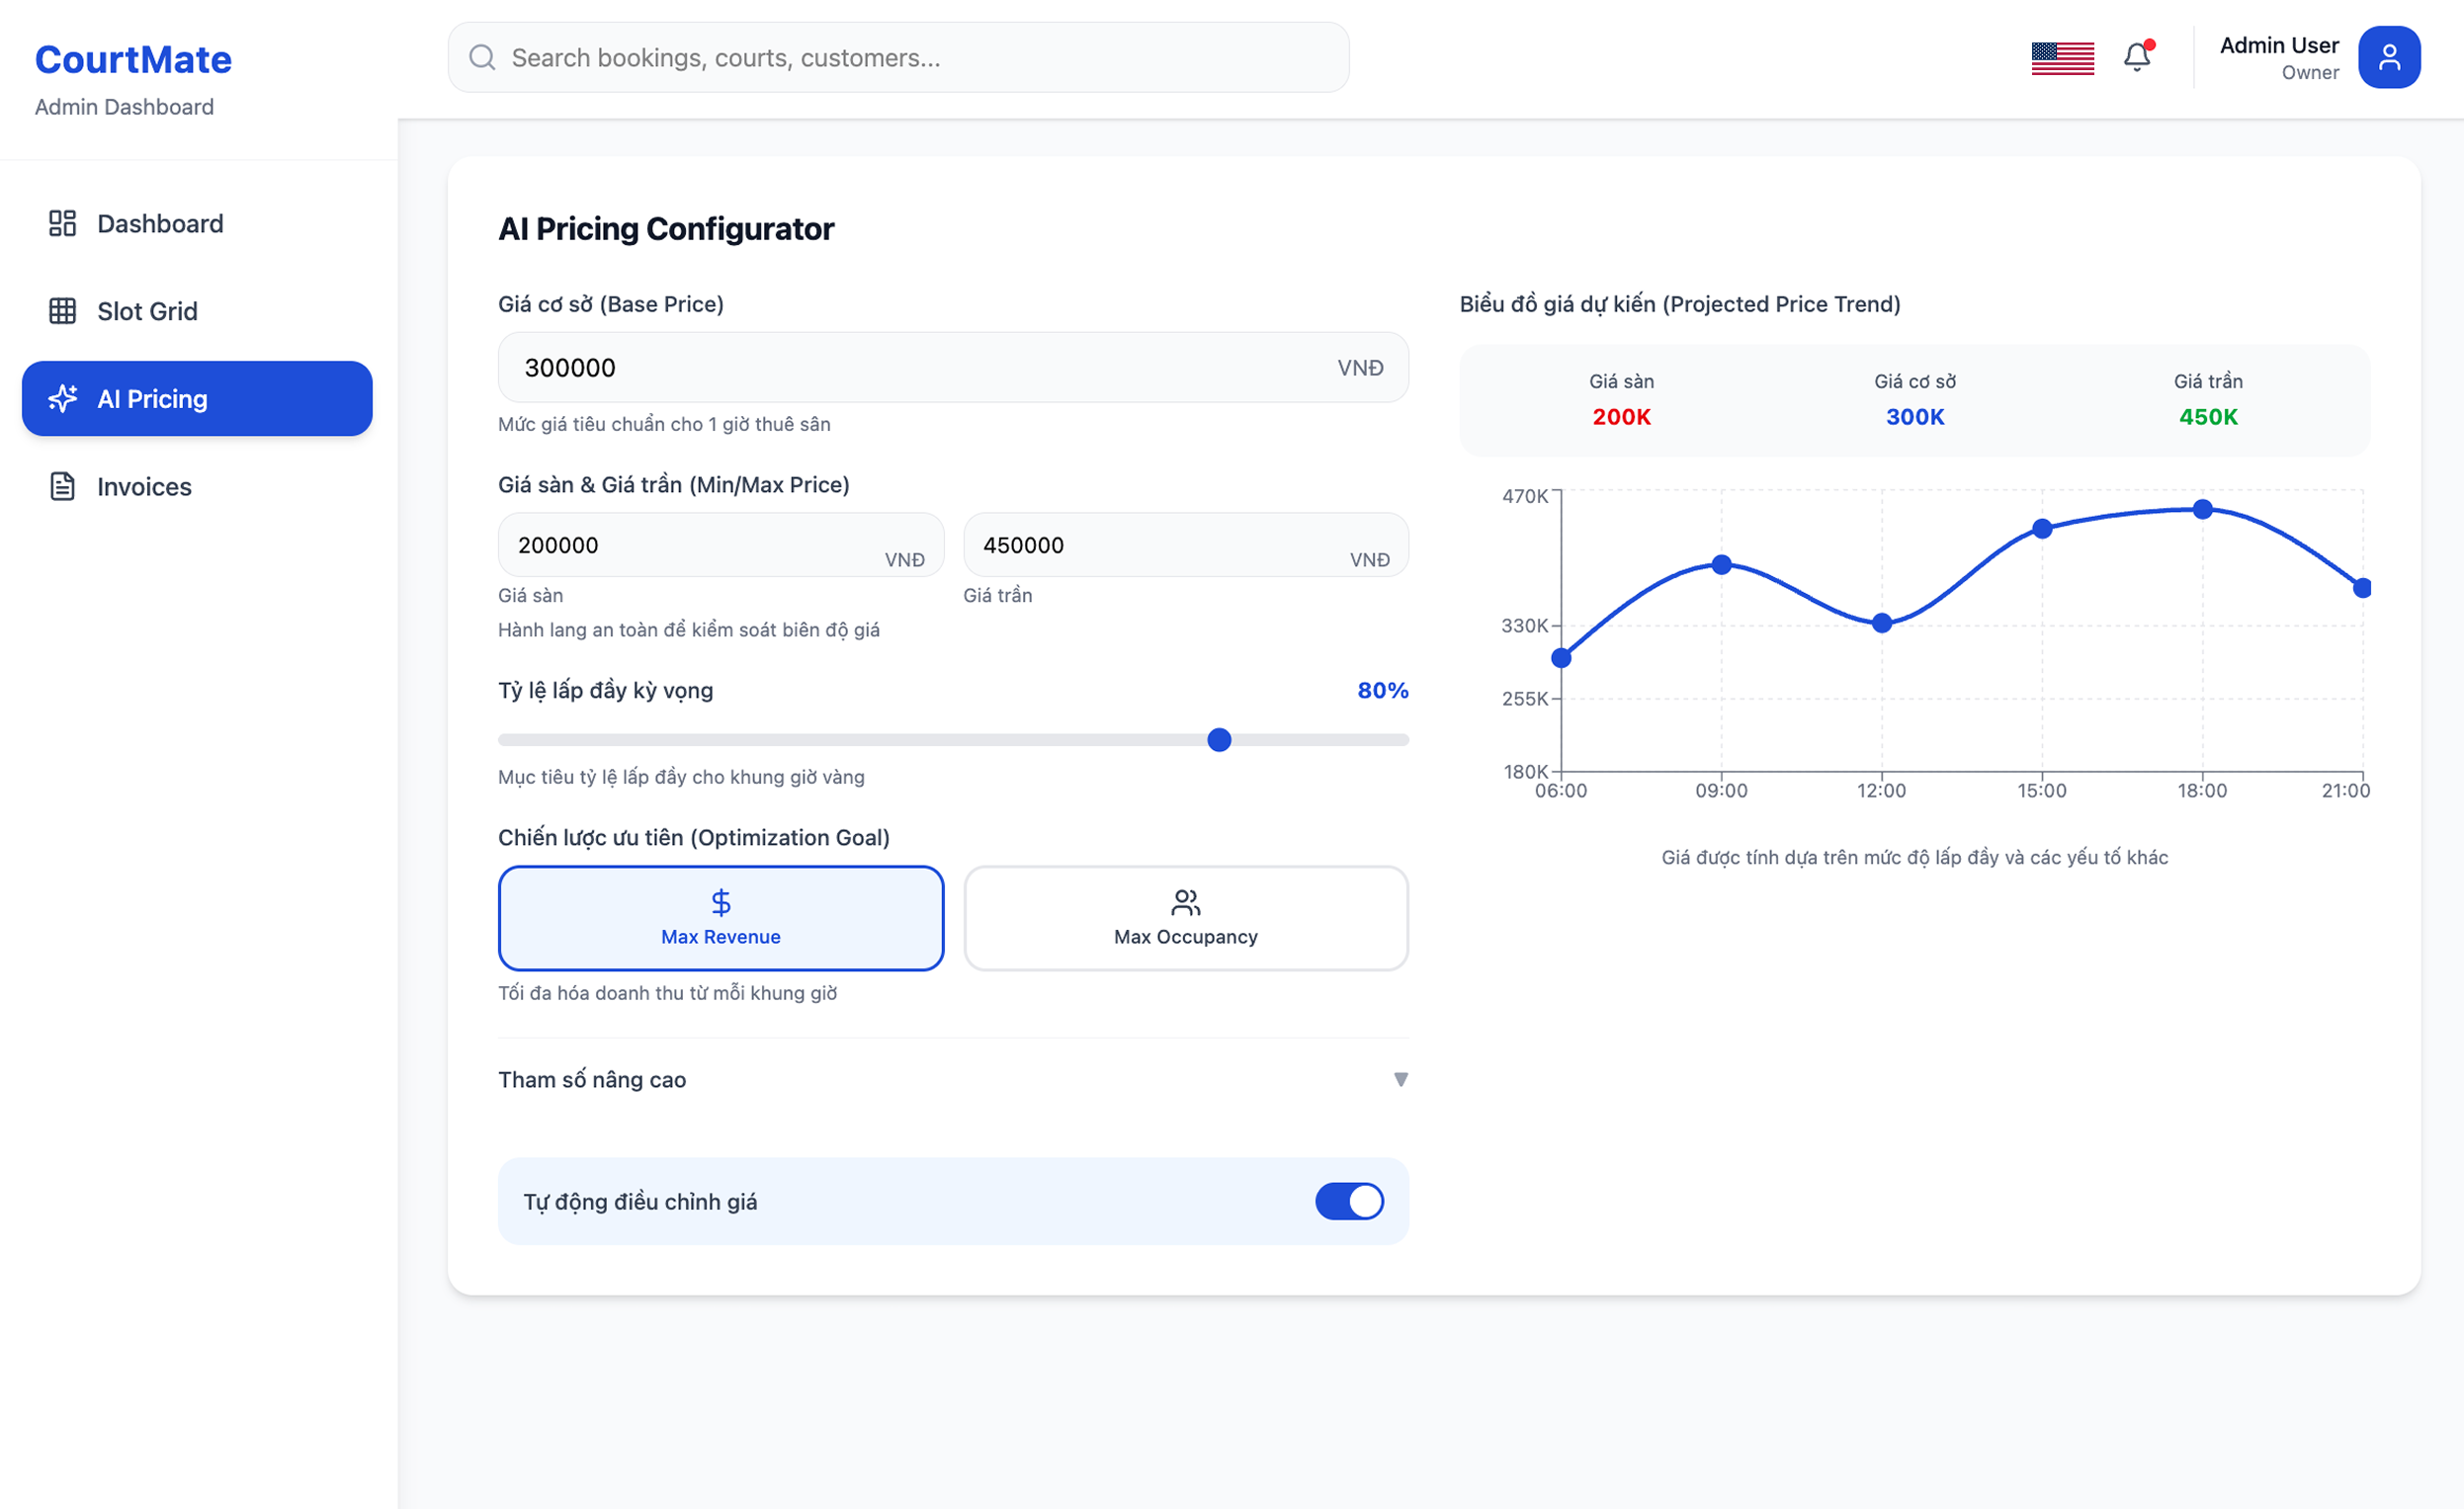
\includegraphics[width=0.8\linewidth]{Images/hinh_07_ai_pricing_config.png}
        \caption{Giao diện Cấu hình Định giá AI (AI Pricing Configurator) kèm biểu đồ dự kiến biến động giá.}
        \label{fig:ai_pricing}
    \end{figure}

    \item \textbf{ERP Integration Sync (Quản lý và Đồng bộ Hóa đơn MISA)} \textit{(Bao gồm 1 màn hình: Invoice Management)}
    \begin{itemize}
        \item \textit{Layout:} Bảng dữ liệu (Data Table) quản lý danh sách chứng từ, tích hợp thanh tìm kiếm và bộ lọc.
        \item \textit{Components:} Nhãn trạng thái (Synced, Pending, Error); Biểu đồ nhỏ hiển thị Connection Status (Tỉ lệ thành công, Lần đồng bộ cuối); Nút "Manual Sync" / "Sync All Pending".
        \item \textit{Flow:} Mở tab Invoices $\rightarrow$ Hệ thống tự động truy xuất các giao dịch chờ xuất hóa đơn $\rightarrow$ Nhấn Sync $\rightarrow$ Backend gọi API sang MISA meInvoice $\rightarrow$ Trả về UUID và cập nhật trạng thái hóa đơn thành Synced.
    \end{itemize}
    \begin{figure}[h!]
        \centering
        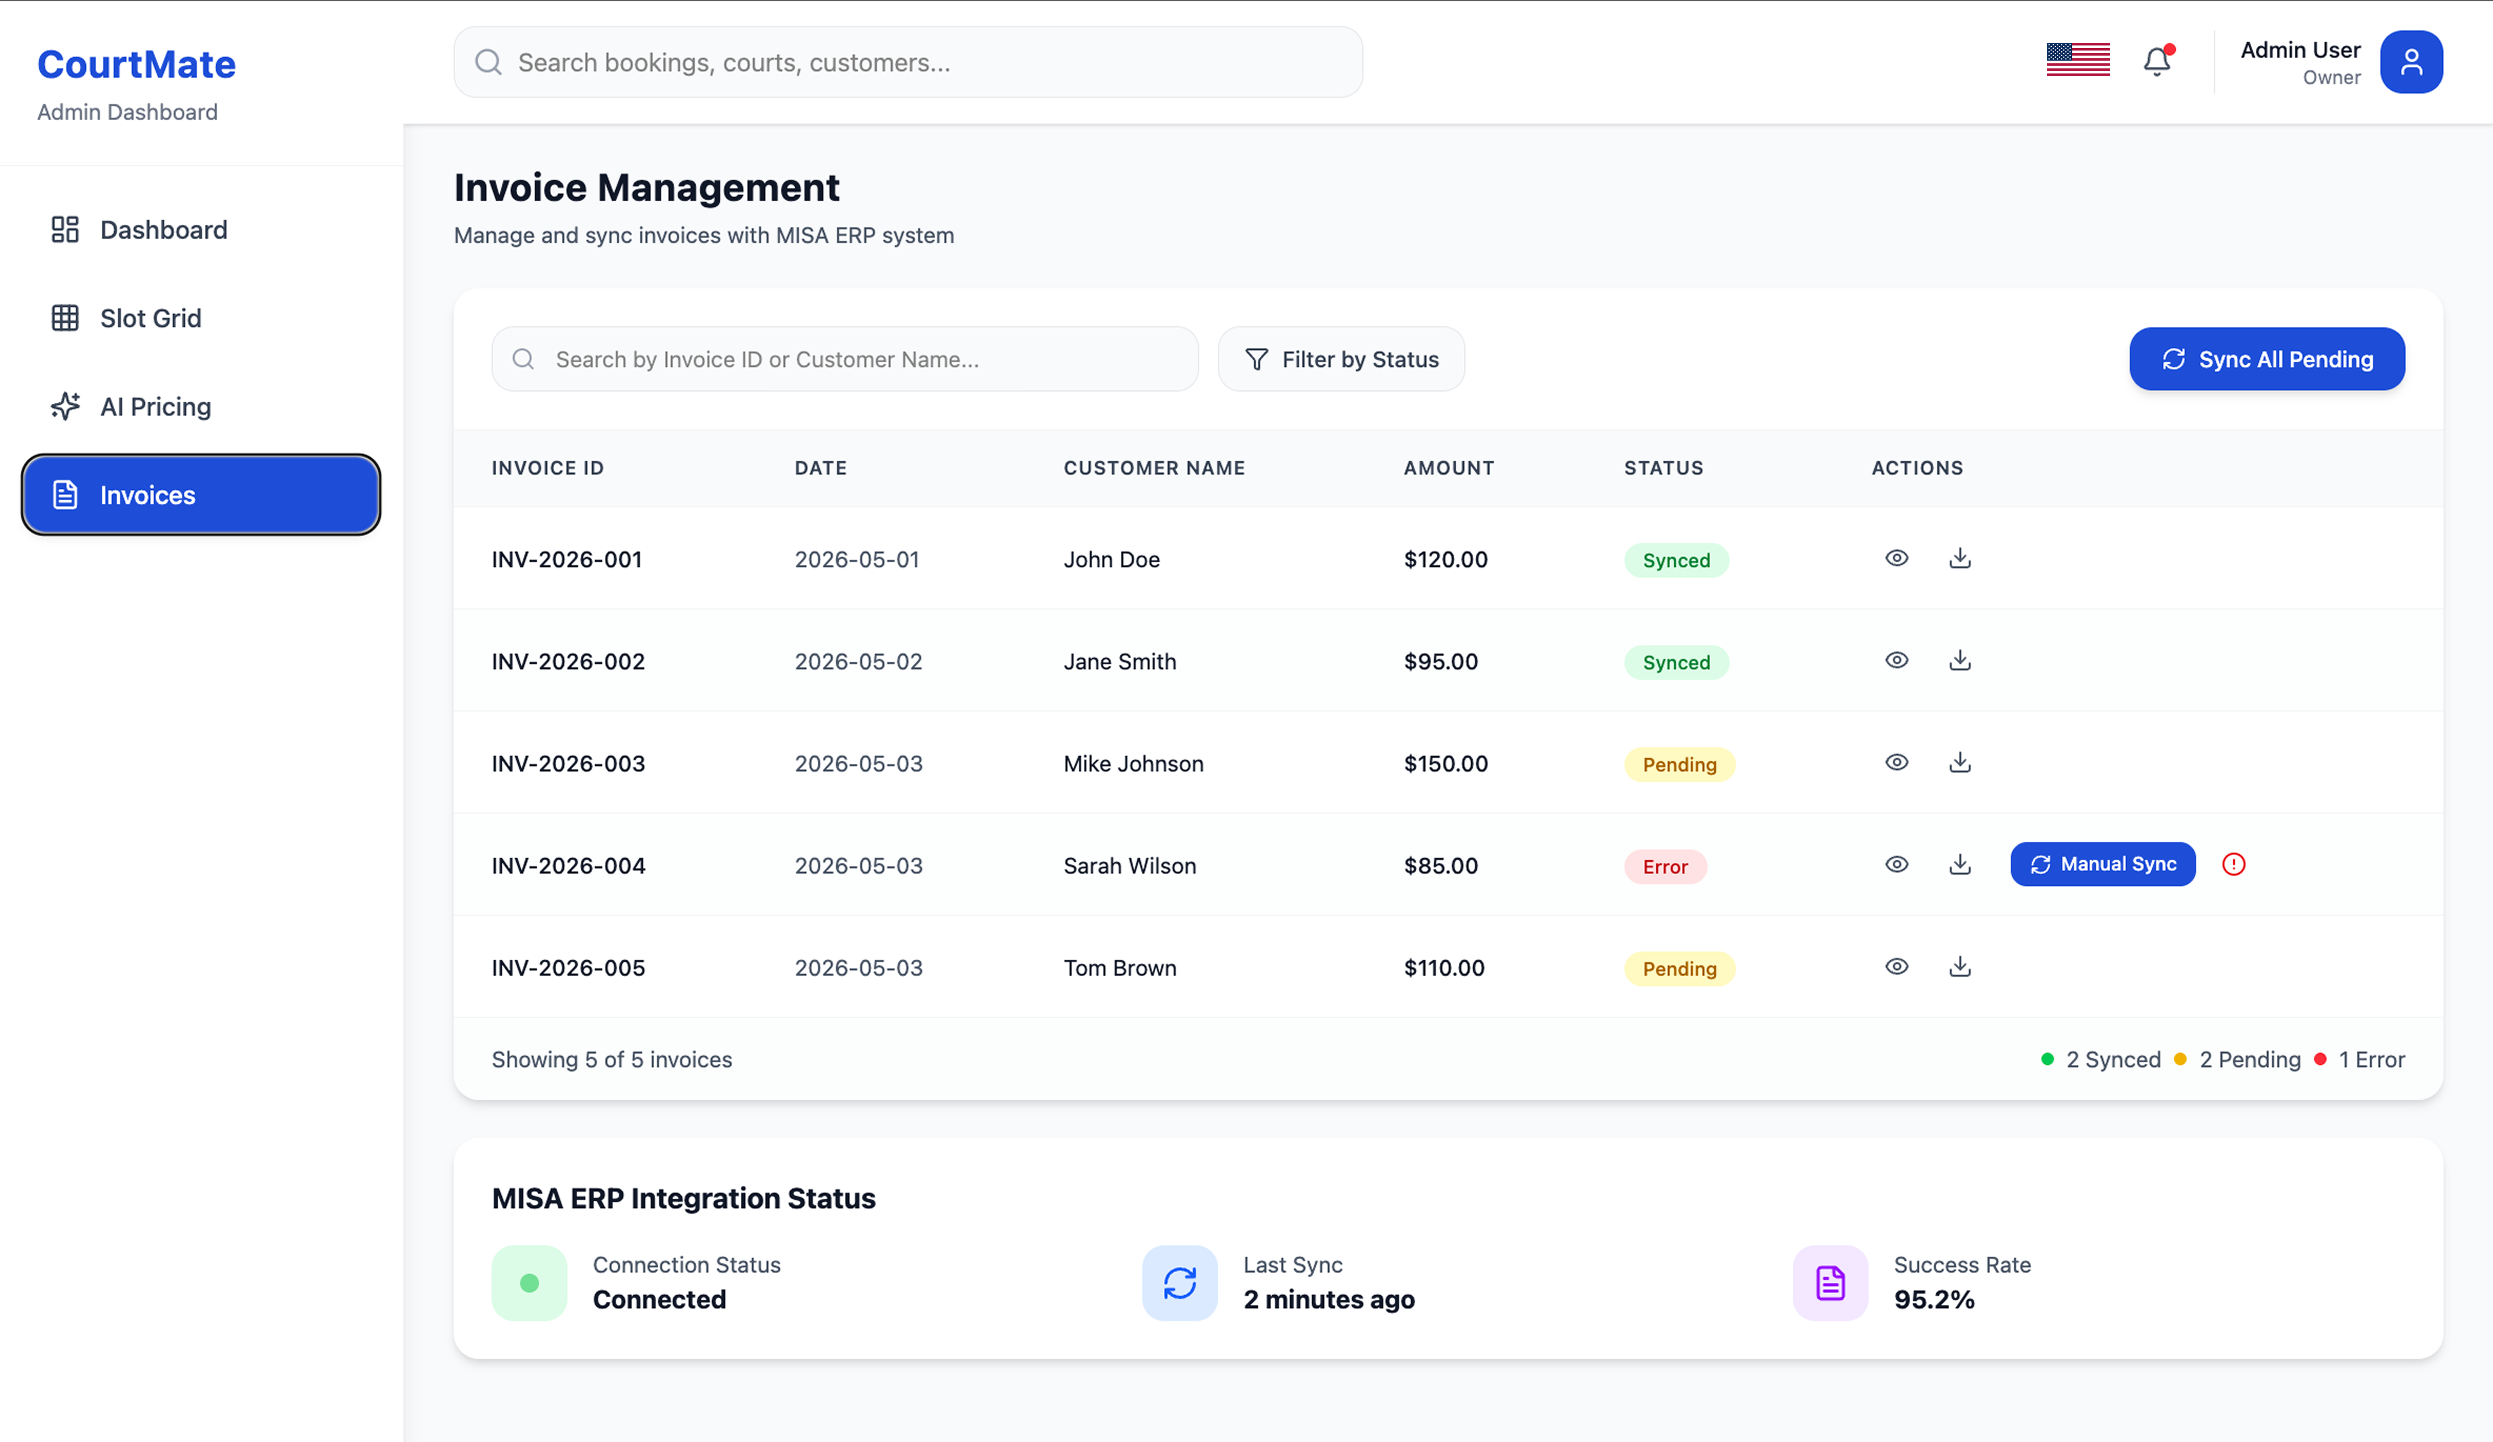
\includegraphics[width=\linewidth]{Images/hinh_08_invoice_management.png}
        \caption{Hệ thống Quản lý Hóa đơn điện tử, tích hợp đối soát và đồng bộ trực tiếp sang nền tảng MISA ERP.}
        \label{fig:misa_erp}
    \end{figure}

    \item \textbf{Luồng Nâng cấp Dịch vụ (B2B Subscription Upgrade)} \textit{(Bao gồm 2 màn hình: Alert tại Dashboard, Giao dịch thành công CourtMate Pro)}
    \begin{itemize}
        \item \textit{Layout:} Banner thông báo tích hợp ngay trên Dashboard, tiếp nối bởi trang xác nhận giao dịch thành công (Success Page).
        \item \textit{Components:} Banner cảnh báo ("Gói dịch vụ sẽ hết hạn sau X ngày"); Nút CTA "Gia hạn ngay"; Biên lai điện tử hiển thị mã giao dịch, thời hạn gói và tổng tiền thanh toán.
        \item \textit{Flow:} Chủ sân nhận thông báo sắp hết hạn phần mềm $\rightarrow$ Click "Gia hạn ngay" $\rightarrow$ Thực hiện thanh toán $\rightarrow$ Hệ thống trả về giao diện Thanh toán thành công (CourtMate Pro - 6 tháng) $\rightarrow$ Tùy chọn Tải biên lai (PDF) hoặc Quay về Dashboard.
    \end{itemize}
    \begin{figure}[h!]
        \centering
        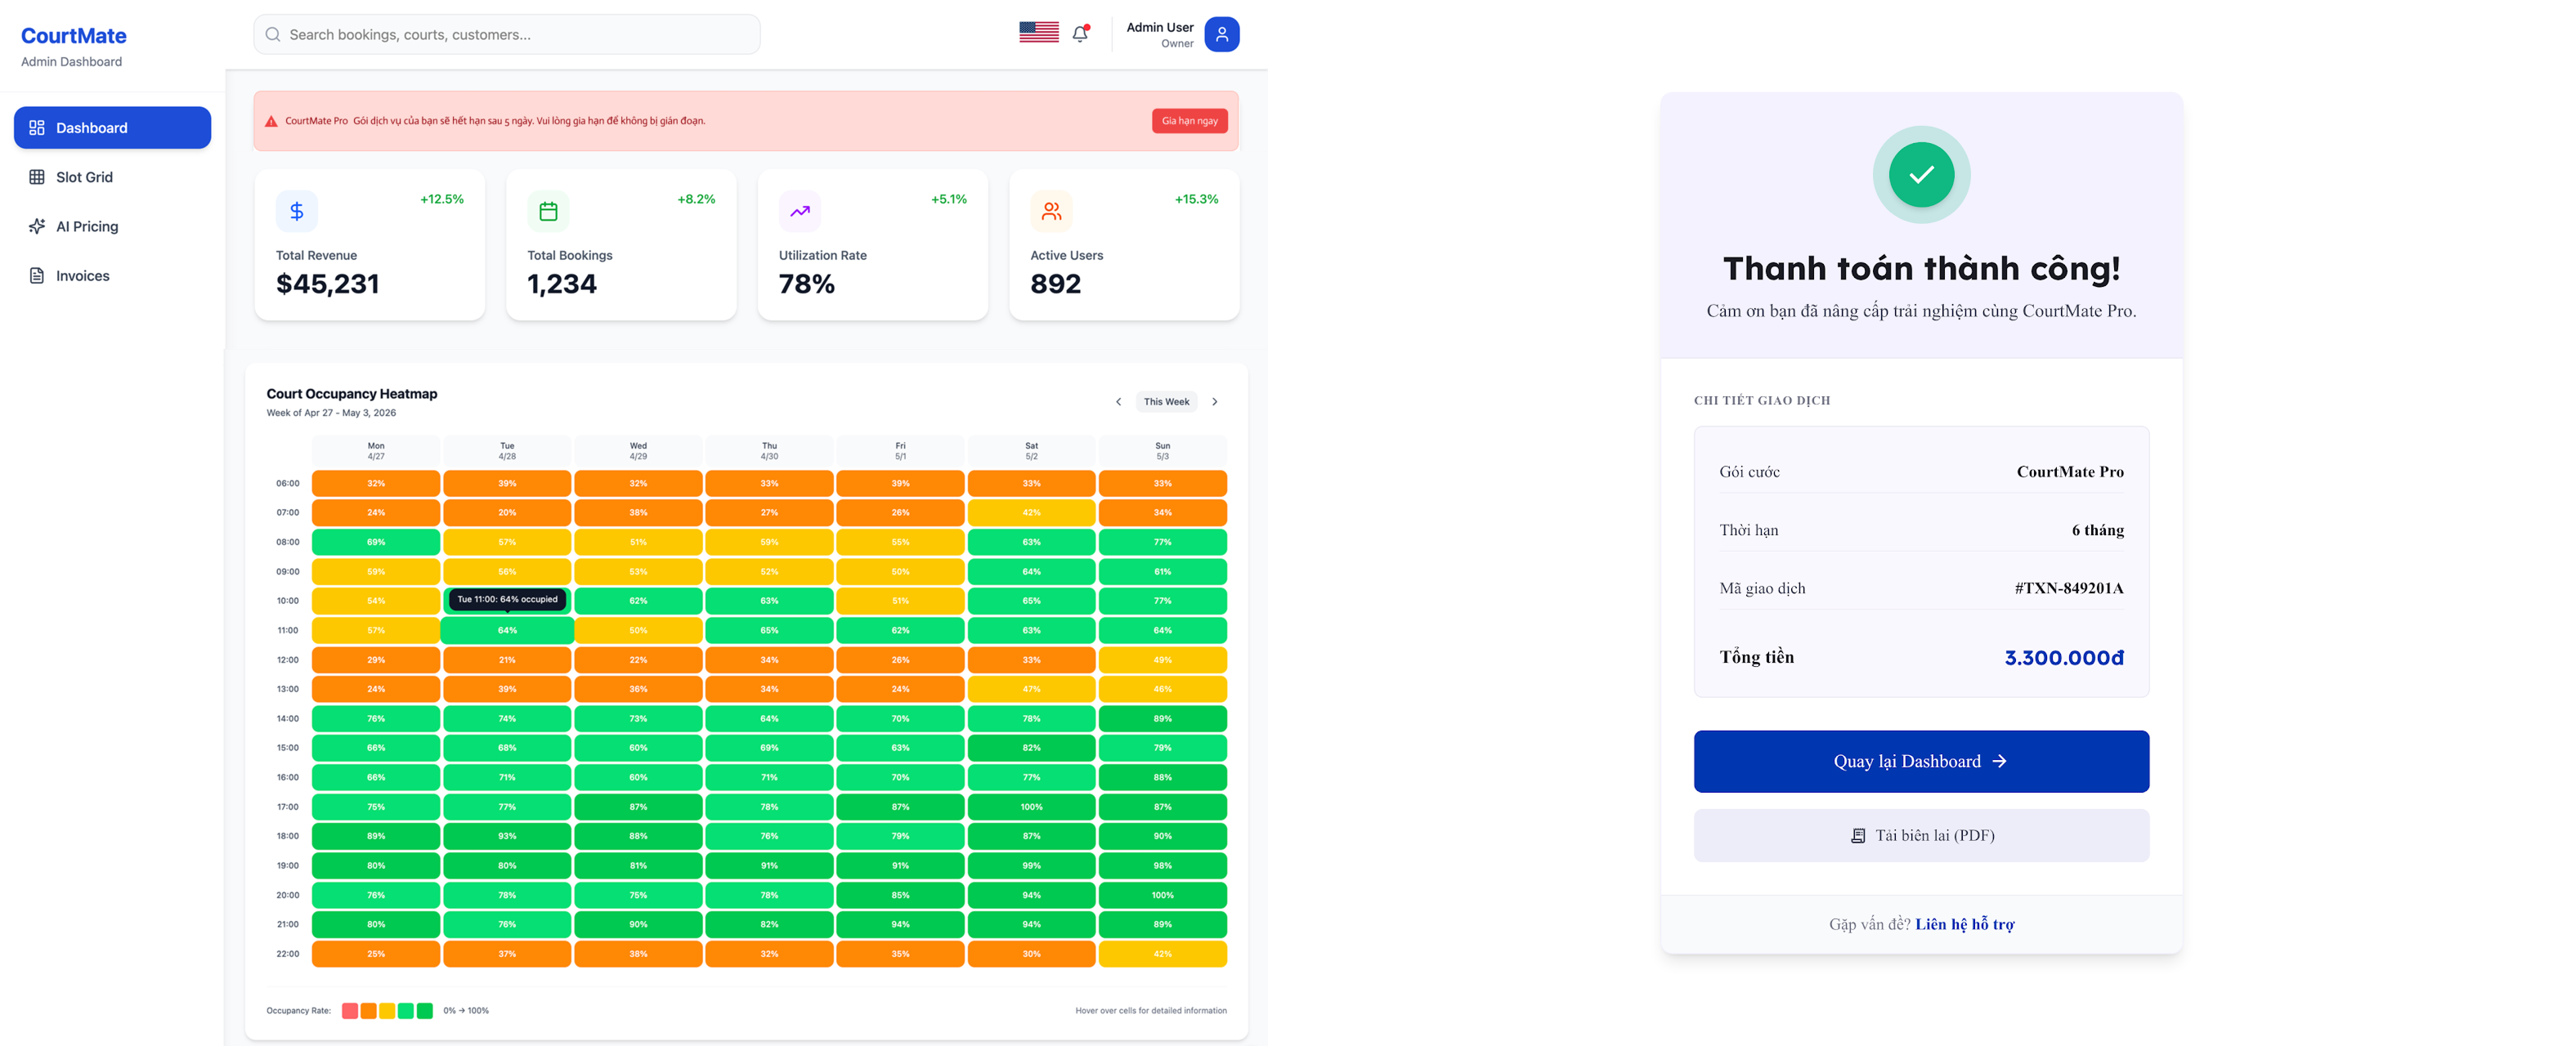
\includegraphics[width=0.8\linewidth]{Images/hinh_09_nang_cap_b2b.png}
        \caption{Luồng nâng cấp và biên lai thanh toán thành công gói dịch vụ CourtMate Pro dành cho Chủ sân.}
        \label{fig:upgrade_b2b}
    \end{figure}
\end{enumerate}

\subsection{Luồng hiện thực AI Dynamic Pricing (Định giá Động)}
Tính năng định giá động được hiện thực hóa thông qua quy trình giao tiếp REST API nội bộ, đảm bảo tính tinh gọn, hiệu năng cao và khả năng mở rộng:

\begin{enumerate}
    \item \textbf{Kích hoạt (Trigger):} Quá trình tính toán được kích hoạt tự động theo chu kỳ hoặc thông qua thao tác thủ công từ Admin trên B2B Service.
    \item \textbf{Tính toán (AI Computation):} B2B Service thực thi một luồng gọi Internal REST API, truyền các tham số ngữ cảnh (vị trí, thời tiết, tỷ lệ lấp đầy) đến AI Engine Service (FastAPI). Tại đây, AI Service chạy thuật toán phân tích (rules-based) và trả về một Hệ số nhân giá (Multiplier).
    \item \textbf{Cập nhật và Lưu trữ (Persistence):} Ngay sau khi nhận kết quả, B2B Service tiến hành lệnh Bulk Update trực tiếp vào trường \texttt{slots.price} của các suất chơi tương ứng trong cơ sở dữ liệu PostgreSQL dùng chung.
\end{enumerate}

\subsection{Thiết kế Dữ liệu và Thực thể Cốt lõi}

\begin{figure}[H]
    \centering
    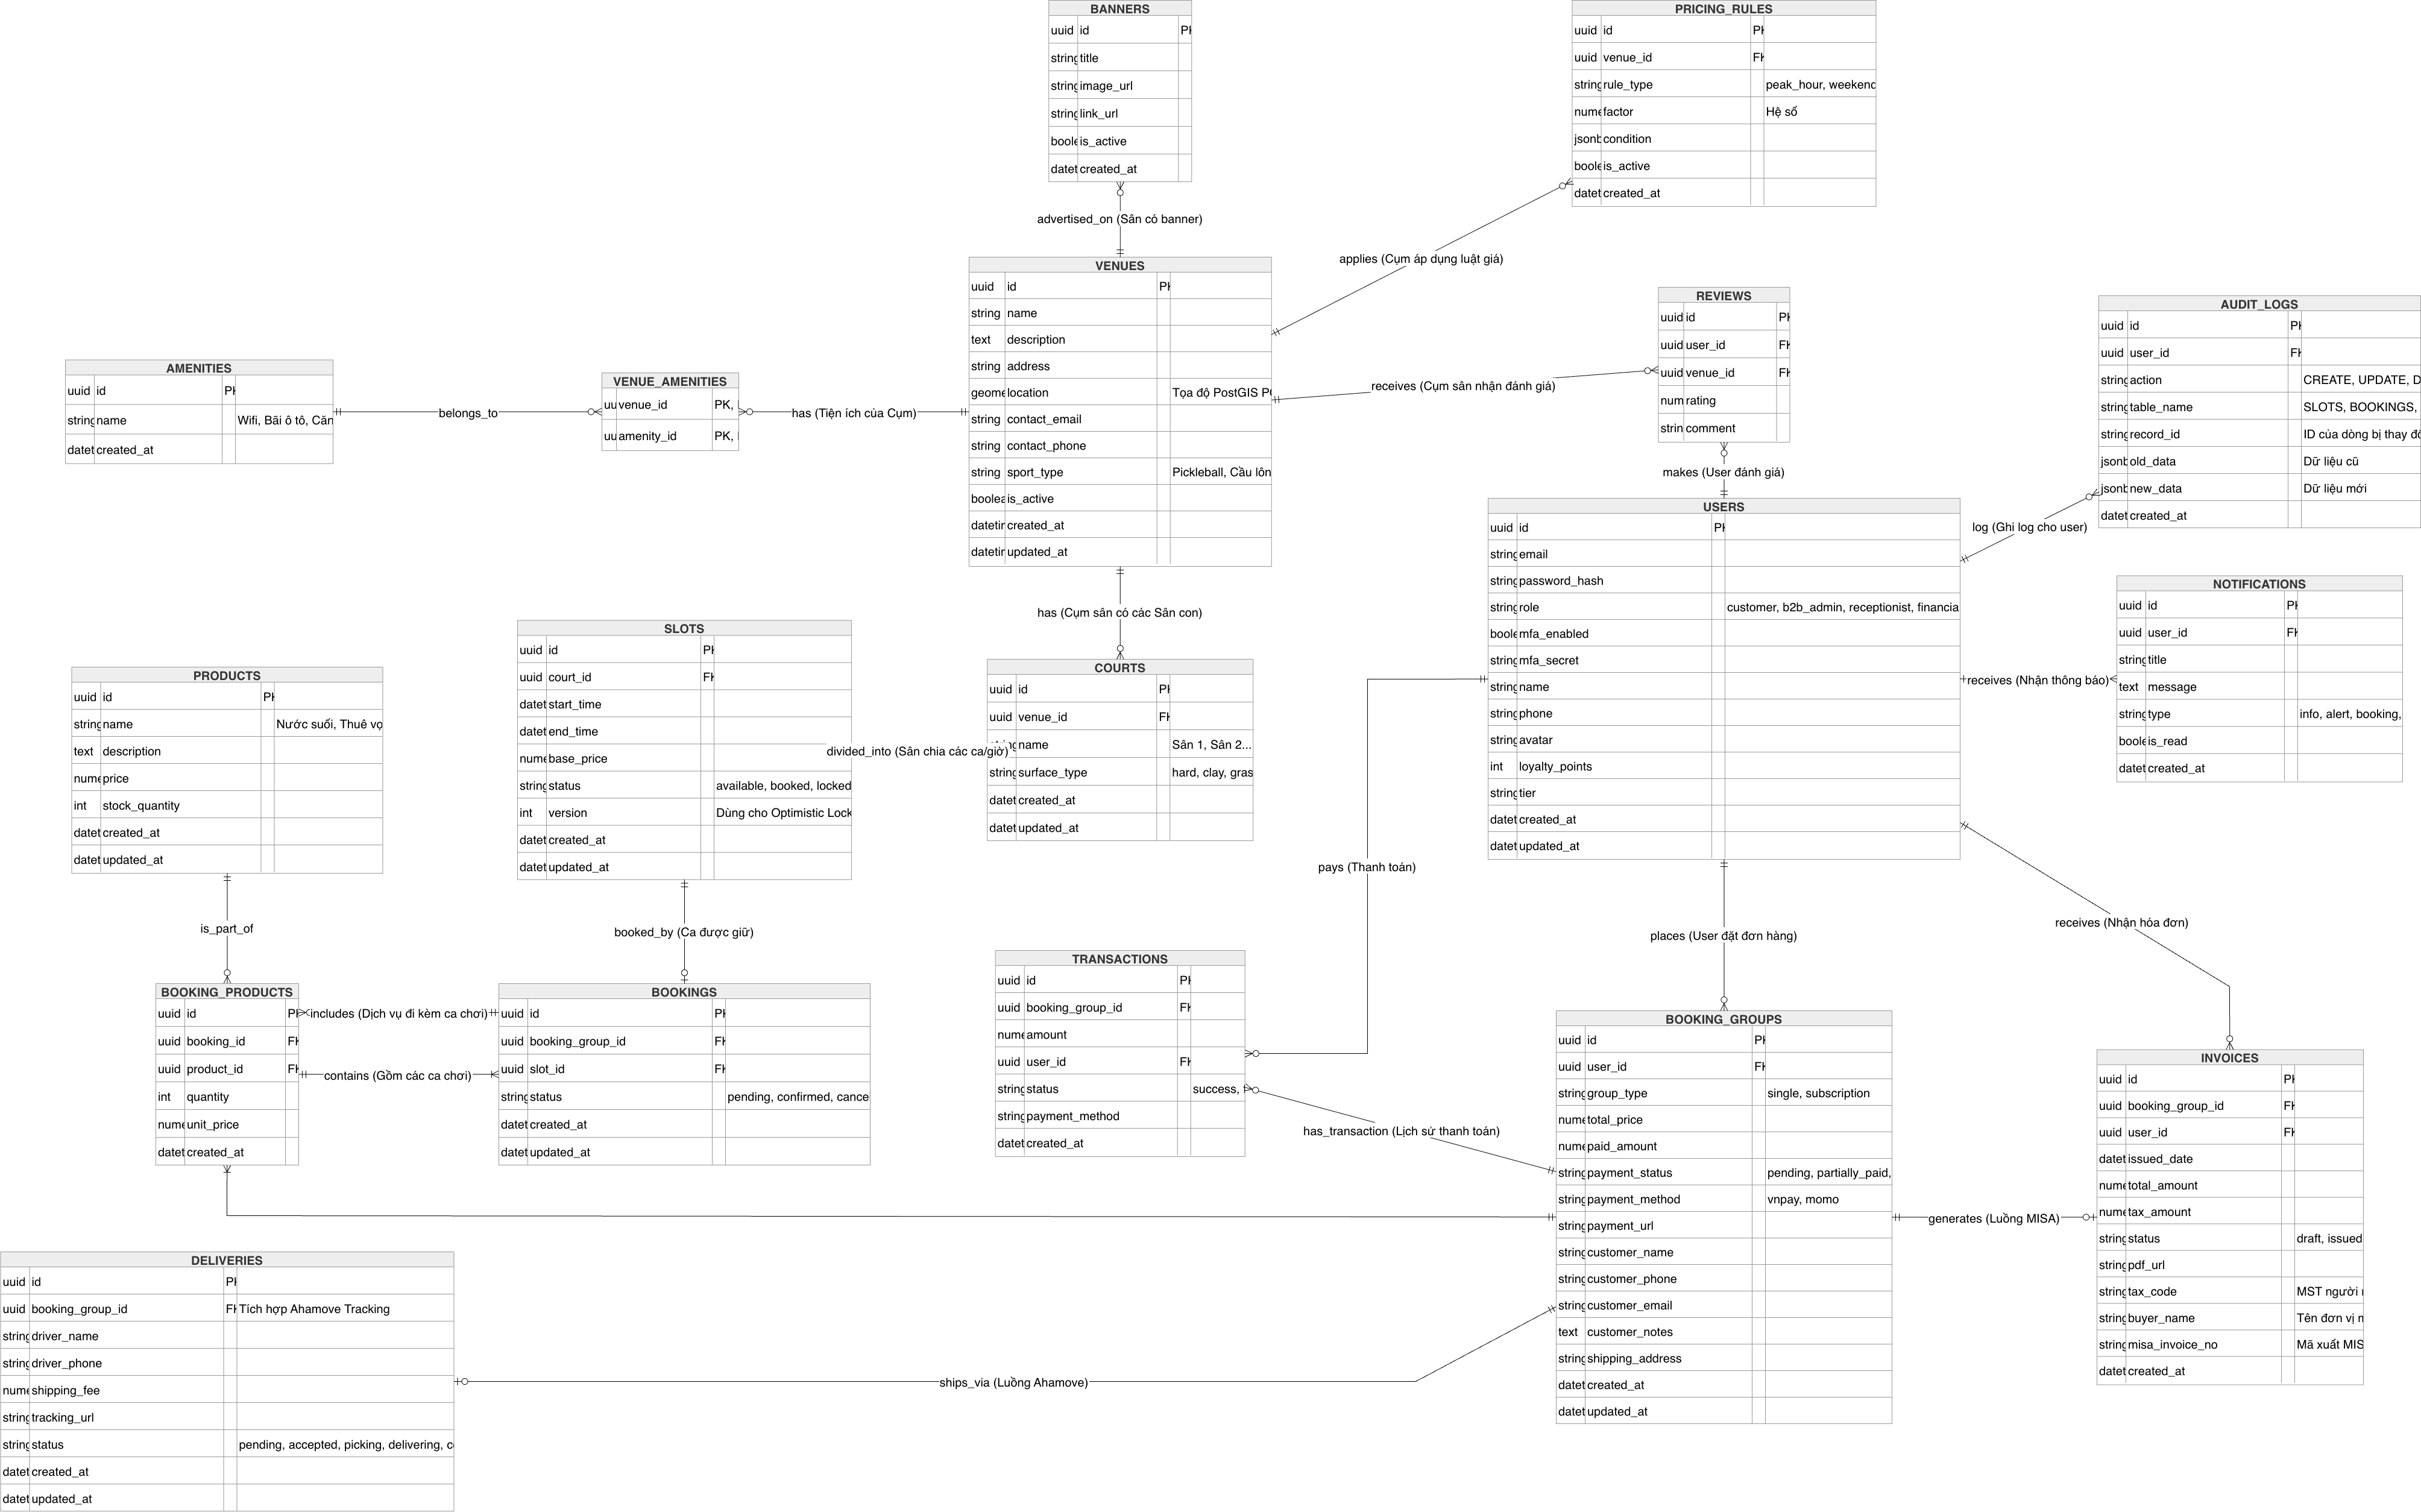
\includegraphics[width=1\textwidth]{Images/eerd.png}
    \caption{Sơ đồ Thực thể - Kết hợp mở rộng (EERD) của hệ thống CourtMate}
    \label{fig:eerd_diagram}
\end{figure}

Hình \ref{fig:eerd_diagram} minh họa sơ đồ Thực thể - Kết hợp mở rộng (EERD) của hệ thống CourtMate, mô tả cấu trúc dữ liệu nền tảng và các mối quan hệ nghiệp vụ phức tạp trong hệ sinh thái đặt sân thể thao trực tuyến.

\subsubsection{Chi tiết các thực thể cốt lõi}
Nhằm tối ưu hóa luồng dữ liệu, các thực thể chính và vai trò của chúng được hệ thống hóa như sau:

\begin{itemize}
    \item \textbf{Bookings (Trung tâm giao dịch):} Lưu trữ toàn bộ thông tin đặt sân. Mỗi Booking thiết lập quan hệ (N:1) với một \textbf{User} và một \textbf{Slot}, đóng vai trò là cơ sở dữ liệu gốc (Single Source of Truth) phục vụ truy vết trạng thái thanh toán và check-in.
    \item \textbf{Slots (Đơn vị suất chơi):} Đại diện cho các khung giờ khả dụng. Slots trực thuộc \textbf{Court}, và Court trực thuộc \textbf{Venue}, hình thành cấu trúc dữ liệu phân cấp 3 tầng chặt chẽ (\textit{Venue $\rightarrow$ Court $\rightarrow$ Slot}).
    \item \textbf{Users (Định danh và Phân quyền):} Tích hợp cơ chế Quản lý Truy cập Dựa trên Vai trò (RBAC) với các phân quyền Player, Owner và Admin, đảm bảo tính đóng gói và an toàn dữ liệu giữa phân hệ B2C và B2B.
\end{itemize}

\subsubsection{Phân nhóm chức năng và Thuộc tính mở rộng}
Hệ thống tổ chức dữ liệu theo các nhóm chức năng độc lập nhằm đảm bảo tính mô-đun (modularity) cao:

\begin{enumerate}
    \item \textbf{Nhóm Vận hành thời gian thực:} Tích hợp các thuộc tính như \texttt{status} (available, locked, booked) và \texttt{locked\_until} để phục vụ trực tiếp cho cơ chế \textit{Optimistic Locking}, triệt tiêu rủi ro Overbooking.
    \item \textbf{Nhóm Tài chính và Hậu cần:} Quản lý vòng đời tài chính thông qua việc liên kết \textbf{Bookings} với các thực thể \textbf{Payments}, \textbf{Transactions} và \textbf{Invoices} (Hóa đơn điện tử), tạo nền tảng cho công tác đối soát tự động và tích hợp MISA ERP.
    \item \textbf{Nhóm Tương tác và Mở rộng:} Các thực thể \textbf{Reviews} (đánh giá), \textbf{Matchmaking} (ghép trận) và cấu hình \textbf{Pricing} (định giá động) được thiết kế tách biệt, cho phép nâng cấp tính năng linh hoạt mà không gây xáo trộn kiến trúc lõi.
\end{enumerate}

Việc áp dụng nguyên tắc chuẩn hóa dữ liệu kết hợp với kiến trúc \textbf{Shared Database Pattern} không chỉ giảm thiểu dư thừa dữ liệu mà còn tối ưu hóa các truy vấn Join phức tạp, phục vụ đắc lực cho công tác trích xuất báo cáo doanh thu và phân tích hành vi người dùng.

\subsection{Đánh giá Hiệu năng và Độ ổn định}
Do kiến trúc hệ thống đã được tinh giản hóa, trọng tâm của công tác đánh giá được đặt vào tính toàn vẹn của logic nghiệp vụ và khả năng chịu tải của cơ sở dữ liệu dùng chung (Shared Database). Các đợt kiểm thử nội bộ minh chứng rằng hệ thống vận hành trơn tru trên cấu hình hạ tầng hiện tại; thời gian phản hồi cho các luồng truy vấn tìm kiếm và đặt sân luôn được duy trì ở mức tối ưu, hoàn toàn đáp ứng được tiêu chuẩn khắt khe của một nền tảng thương mại điện tử.

\subsection{Kế hoạch Quản lý Rủi ro Hệ thống}
Nhằm đảm bảo tính bền vững và tính sẵn sàng cao (High Availability) cho CourtMate, nhóm phát triển đã thiết lập một khung quản lý rủi ro chuyên sâu, bám sát các đặc thù của kiến trúc Microservices và cơ sở dữ liệu tập trung:

\begin{table}[H]
    \centering
    \renewcommand{\arraystretch}{1.4}
    \begin{tabularx}{\textwidth}{|c|p{4cm}|c|X|}
    \hline
    \textbf{STT} & \textbf{Tên rủi ro} & \textbf{Mức độ} & \textbf{Chiến lược phòng ngừa \& giải pháp xử lý} \\ \hline
    1 & Quá tải Shared Database khi kiểm thử tải cực đại (Stress Test) & Cao & Tối ưu hóa Database Indexing, triển khai Connection Pooling và thiết lập Resource Limits (giới hạn tài nguyên) cho từng service truy cập. \\ \hline
    2 & Trễ tiến độ tích hợp API bên thứ 3 (VietQR, MISA) & Trung bình & Xây dựng Adapter Service tích hợp cơ chế Retry logic và Circuit Breaker; ứng dụng Mock API trong pha phát triển. \\ \hline
    3 & Vượt ngân sách hạ tầng Cloud (Free Tier) & Thấp & Cấu hình Budget Alerts trên nền tảng AWS/GCP; tối ưu dung lượng Docker Image và tự động hóa việc tắt các service không thiết yếu. \\ \hline
    4 & Lỗi Race Condition dẫn đến Overbooking & Cao & Triển khai Database-level Optimistic Lock thông qua trường \texttt{locked\_until} hoặc áp dụng kỹ thuật Versioning trong quá trình thanh toán. \\ \hline
    \end{tabularx}
    \caption{Bảng Kế hoạch quản lý rủi ro hệ thống CourtMate}
    \label{tab:risk_management}
\end{table}
\newpage
\input{Contents/Part5_Implementation/Part5_SystemDesign.tex}
\newpage
\newpage

%%%%%%%%%%%%%%%%% OUTRO %%%%%%%%%%%%%%%%%%%
\addcontentsline{toc}{section}{Tài liệu tham khảo}

\renewcommand{\refname}{Tài liệu tham khảo}
\begin{thebibliography}{99}
    \bibitem{ref:laudon} K. C. Laudon and C. G. Traver, \textit{E-commerce 2021-2022: Business, Technology, Society}, 17th ed., Pearson, 2021.
    \bibitem{ref:schneider} G. P. Schneider, \textit{Electronic Commerce}, 12th ed., Cengage Learning, 2017.
    \bibitem{ref:quang} Nguyễn Đăng Quang, \textit{Giáo trình Thương mại điện tử}, NXB Đại học Quốc gia TP.HCM, 2020.
    \bibitem{ref:google} Google, "Google Maps Platform Documentation," Google Cloud, 2024.
    \bibitem{ref:misa} MISA, "Tài liệu tích hợp API meInvoice," MISA meInvoice, 2024.
    \bibitem{ref:statista} Statista, "Racquet Sports Market Size \& Growth 2024-2028", 2024.
    \bibitem{ref:laodong} Báo Lao Động, "Bùng nổ phong trào Pickleball: Bài toán thiếu hụt sân bãi," 2024.
    \bibitem{ref:playtomic} Playtomic, "Playtomic Manager Pricing," 2024.
    \bibitem{ref:courtreserve} CourtReserve, "Pricing for Tennis \& Pickleball Software," 2024.
    \bibitem{ref:alobo} ALOBO, "Phần mềm chuyên biệt quản lý sân thể thao," 2024.
    \bibitem{ref:gartner} Gartner, "The B2B Buying Journey," 2024.
    \bibitem{ref:wearesocial} We Are Social \& Meltwater, "Digital 2024: Vietnam," 2024.
    \bibitem{ref:kotler} P. Kotler, "Marketing 4.0: Moving from Traditional to Digital," 2017.
    \bibitem{ref:aws} Amazon Web Services, "AWS Pricing," 2024.
    \bibitem{ref:bizfly} Bizfly Cloud, "Bảng giá dịch vụ Cloud Server," 2024.
    \bibitem{ref:viettel} Viettel IDC, "Báo giá dịch vụ Viettel Cloud Server," 2024.
\end{thebibliography}
\newpage
\input{Outro/PhuLuc}
\end{document}

